% Options for packages loaded elsewhere
\PassOptionsToPackage{unicode}{hyperref}
\PassOptionsToPackage{hyphens}{url}
\PassOptionsToPackage{dvipsnames,svgnames,x11names}{xcolor}
%
\documentclass[
  a4paper,
]{book}

\usepackage{amsmath,amssymb}
\usepackage{iftex}
\ifPDFTeX
  \usepackage[T1]{fontenc}
  \usepackage[utf8]{inputenc}
  \usepackage{textcomp} % provide euro and other symbols
\else % if luatex or xetex
  \usepackage{unicode-math}
  \defaultfontfeatures{Scale=MatchLowercase}
  \defaultfontfeatures[\rmfamily]{Ligatures=TeX,Scale=1}
\fi
\usepackage{lmodern}
\ifPDFTeX\else  
    % xetex/luatex font selection
\fi
% Use upquote if available, for straight quotes in verbatim environments
\IfFileExists{upquote.sty}{\usepackage{upquote}}{}
\IfFileExists{microtype.sty}{% use microtype if available
  \usepackage[]{microtype}
  \UseMicrotypeSet[protrusion]{basicmath} % disable protrusion for tt fonts
}{}
\makeatletter
\@ifundefined{KOMAClassName}{% if non-KOMA class
  \IfFileExists{parskip.sty}{%
    \usepackage{parskip}
  }{% else
    \setlength{\parindent}{0pt}
    \setlength{\parskip}{6pt plus 2pt minus 1pt}}
}{% if KOMA class
  \KOMAoptions{parskip=half}}
\makeatother
\usepackage{xcolor}
\usepackage[paperwidth=8.27in,paperheight=11.69in,left=1.25in,textwidth=
5.25in,top=1.00in,textheight=8.25in]{geometry}
\setlength{\emergencystretch}{3em} % prevent overfull lines
\setcounter{secnumdepth}{5}
% Make \paragraph and \subparagraph free-standing
\makeatletter
\ifx\paragraph\undefined\else
  \let\oldparagraph\paragraph
  \renewcommand{\paragraph}{
    \@ifstar
      \xxxParagraphStar
      \xxxParagraphNoStar
  }
  \newcommand{\xxxParagraphStar}[1]{\oldparagraph*{#1}\mbox{}}
  \newcommand{\xxxParagraphNoStar}[1]{\oldparagraph{#1}\mbox{}}
\fi
\ifx\subparagraph\undefined\else
  \let\oldsubparagraph\subparagraph
  \renewcommand{\subparagraph}{
    \@ifstar
      \xxxSubParagraphStar
      \xxxSubParagraphNoStar
  }
  \newcommand{\xxxSubParagraphStar}[1]{\oldsubparagraph*{#1}\mbox{}}
  \newcommand{\xxxSubParagraphNoStar}[1]{\oldsubparagraph{#1}\mbox{}}
\fi
\makeatother

\usepackage{color}
\usepackage{fancyvrb}
\newcommand{\VerbBar}{|}
\newcommand{\VERB}{\Verb[commandchars=\\\{\}]}
\DefineVerbatimEnvironment{Highlighting}{Verbatim}{commandchars=\\\{\}}
% Add ',fontsize=\small' for more characters per line
\usepackage{framed}
\definecolor{shadecolor}{RGB}{241,243,245}
\newenvironment{Shaded}{\begin{snugshade}}{\end{snugshade}}
\newcommand{\AlertTok}[1]{\textcolor[rgb]{0.68,0.00,0.00}{#1}}
\newcommand{\AnnotationTok}[1]{\textcolor[rgb]{0.37,0.37,0.37}{#1}}
\newcommand{\AttributeTok}[1]{\textcolor[rgb]{0.40,0.45,0.13}{#1}}
\newcommand{\BaseNTok}[1]{\textcolor[rgb]{0.68,0.00,0.00}{#1}}
\newcommand{\BuiltInTok}[1]{\textcolor[rgb]{0.00,0.23,0.31}{#1}}
\newcommand{\CharTok}[1]{\textcolor[rgb]{0.13,0.47,0.30}{#1}}
\newcommand{\CommentTok}[1]{\textcolor[rgb]{0.37,0.37,0.37}{#1}}
\newcommand{\CommentVarTok}[1]{\textcolor[rgb]{0.37,0.37,0.37}{\textit{#1}}}
\newcommand{\ConstantTok}[1]{\textcolor[rgb]{0.56,0.35,0.01}{#1}}
\newcommand{\ControlFlowTok}[1]{\textcolor[rgb]{0.00,0.23,0.31}{\textbf{#1}}}
\newcommand{\DataTypeTok}[1]{\textcolor[rgb]{0.68,0.00,0.00}{#1}}
\newcommand{\DecValTok}[1]{\textcolor[rgb]{0.68,0.00,0.00}{#1}}
\newcommand{\DocumentationTok}[1]{\textcolor[rgb]{0.37,0.37,0.37}{\textit{#1}}}
\newcommand{\ErrorTok}[1]{\textcolor[rgb]{0.68,0.00,0.00}{#1}}
\newcommand{\ExtensionTok}[1]{\textcolor[rgb]{0.00,0.23,0.31}{#1}}
\newcommand{\FloatTok}[1]{\textcolor[rgb]{0.68,0.00,0.00}{#1}}
\newcommand{\FunctionTok}[1]{\textcolor[rgb]{0.28,0.35,0.67}{#1}}
\newcommand{\ImportTok}[1]{\textcolor[rgb]{0.00,0.46,0.62}{#1}}
\newcommand{\InformationTok}[1]{\textcolor[rgb]{0.37,0.37,0.37}{#1}}
\newcommand{\KeywordTok}[1]{\textcolor[rgb]{0.00,0.23,0.31}{\textbf{#1}}}
\newcommand{\NormalTok}[1]{\textcolor[rgb]{0.00,0.23,0.31}{#1}}
\newcommand{\OperatorTok}[1]{\textcolor[rgb]{0.37,0.37,0.37}{#1}}
\newcommand{\OtherTok}[1]{\textcolor[rgb]{0.00,0.23,0.31}{#1}}
\newcommand{\PreprocessorTok}[1]{\textcolor[rgb]{0.68,0.00,0.00}{#1}}
\newcommand{\RegionMarkerTok}[1]{\textcolor[rgb]{0.00,0.23,0.31}{#1}}
\newcommand{\SpecialCharTok}[1]{\textcolor[rgb]{0.37,0.37,0.37}{#1}}
\newcommand{\SpecialStringTok}[1]{\textcolor[rgb]{0.13,0.47,0.30}{#1}}
\newcommand{\StringTok}[1]{\textcolor[rgb]{0.13,0.47,0.30}{#1}}
\newcommand{\VariableTok}[1]{\textcolor[rgb]{0.07,0.07,0.07}{#1}}
\newcommand{\VerbatimStringTok}[1]{\textcolor[rgb]{0.13,0.47,0.30}{#1}}
\newcommand{\WarningTok}[1]{\textcolor[rgb]{0.37,0.37,0.37}{\textit{#1}}}

\providecommand{\tightlist}{%
  \setlength{\itemsep}{0pt}\setlength{\parskip}{0pt}}\usepackage{longtable,booktabs,array}
\usepackage{calc} % for calculating minipage widths
% Correct order of tables after \paragraph or \subparagraph
\usepackage{etoolbox}
\makeatletter
\patchcmd\longtable{\par}{\if@noskipsec\mbox{}\fi\par}{}{}
\makeatother
% Allow footnotes in longtable head/foot
\IfFileExists{footnotehyper.sty}{\usepackage{footnotehyper}}{\usepackage{footnote}}
\makesavenoteenv{longtable}
\usepackage{graphicx}
\makeatletter
\def\maxwidth{\ifdim\Gin@nat@width>\linewidth\linewidth\else\Gin@nat@width\fi}
\def\maxheight{\ifdim\Gin@nat@height>\textheight\textheight\else\Gin@nat@height\fi}
\makeatother
% Scale images if necessary, so that they will not overflow the page
% margins by default, and it is still possible to overwrite the defaults
% using explicit options in \includegraphics[width, height, ...]{}
\setkeys{Gin}{width=\maxwidth,height=\maxheight,keepaspectratio}
% Set default figure placement to htbp
\makeatletter
\def\fps@figure{htbp}
\makeatother
% definitions for citeproc citations
\NewDocumentCommand\citeproctext{}{}
\NewDocumentCommand\citeproc{mm}{%
  \begingroup\def\citeproctext{#2}\cite{#1}\endgroup}
\makeatletter
 % allow citations to break across lines
 \let\@cite@ofmt\@firstofone
 % avoid brackets around text for \cite:
 \def\@biblabel#1{}
 \def\@cite#1#2{{#1\if@tempswa , #2\fi}}
\makeatother
\newlength{\cslhangindent}
\setlength{\cslhangindent}{1.5em}
\newlength{\csllabelwidth}
\setlength{\csllabelwidth}{3em}
\newenvironment{CSLReferences}[2] % #1 hanging-indent, #2 entry-spacing
 {\begin{list}{}{%
  \setlength{\itemindent}{0pt}
  \setlength{\leftmargin}{0pt}
  \setlength{\parsep}{0pt}
  % turn on hanging indent if param 1 is 1
  \ifodd #1
   \setlength{\leftmargin}{\cslhangindent}
   \setlength{\itemindent}{-1\cslhangindent}
  \fi
  % set entry spacing
  \setlength{\itemsep}{#2\baselineskip}}}
 {\end{list}}
\usepackage{calc}
\newcommand{\CSLBlock}[1]{\hfill\break\parbox[t]{\linewidth}{\strut\ignorespaces#1\strut}}
\newcommand{\CSLLeftMargin}[1]{\parbox[t]{\csllabelwidth}{\strut#1\strut}}
\newcommand{\CSLRightInline}[1]{\parbox[t]{\linewidth - \csllabelwidth}{\strut#1\strut}}
\newcommand{\CSLIndent}[1]{\hspace{\cslhangindent}#1}

\usepackage{makeidx}
\makeindex
\usepackage{titling}
\usepackage{pdfpages}
\usepackage{atbegshi}% http://ctan.org/pkg/atbegshi
\let\oldmaketitle\maketitle
\AtBeginDocument{\let\maketitle\relax}
\AtBeginDocument{\AtBeginShipoutNext{\AtBeginShipoutDiscard}} % Discard next blank page

\makeatletter
\@ifpackageloaded{tcolorbox}{}{\usepackage[skins,breakable]{tcolorbox}}
\@ifpackageloaded{fontawesome5}{}{\usepackage{fontawesome5}}
\definecolor{quarto-callout-color}{HTML}{909090}
\definecolor{quarto-callout-note-color}{HTML}{0758E5}
\definecolor{quarto-callout-important-color}{HTML}{CC1914}
\definecolor{quarto-callout-warning-color}{HTML}{EB9113}
\definecolor{quarto-callout-tip-color}{HTML}{00A047}
\definecolor{quarto-callout-caution-color}{HTML}{FC5300}
\definecolor{quarto-callout-color-frame}{HTML}{acacac}
\definecolor{quarto-callout-note-color-frame}{HTML}{4582ec}
\definecolor{quarto-callout-important-color-frame}{HTML}{d9534f}
\definecolor{quarto-callout-warning-color-frame}{HTML}{f0ad4e}
\definecolor{quarto-callout-tip-color-frame}{HTML}{02b875}
\definecolor{quarto-callout-caution-color-frame}{HTML}{fd7e14}
\makeatother
\makeatletter
\@ifpackageloaded{bookmark}{}{\usepackage{bookmark}}
\makeatother
\makeatletter
\@ifpackageloaded{caption}{}{\usepackage{caption}}
\AtBeginDocument{%
\ifdefined\contentsname
  \renewcommand*\contentsname{Índice}
\else
  \newcommand\contentsname{Índice}
\fi
\ifdefined\listfigurename
  \renewcommand*\listfigurename{Lista de Figuras}
\else
  \newcommand\listfigurename{Lista de Figuras}
\fi
\ifdefined\listtablename
  \renewcommand*\listtablename{Lista de Tabelas}
\else
  \newcommand\listtablename{Lista de Tabelas}
\fi
\ifdefined\figurename
  \renewcommand*\figurename{Figura}
\else
  \newcommand\figurename{Figura}
\fi
\ifdefined\tablename
  \renewcommand*\tablename{Tabela}
\else
  \newcommand\tablename{Tabela}
\fi
}
\@ifpackageloaded{float}{}{\usepackage{float}}
\floatstyle{ruled}
\@ifundefined{c@chapter}{\newfloat{codelisting}{h}{lop}}{\newfloat{codelisting}{h}{lop}[chapter]}
\floatname{codelisting}{Listagem}
\newcommand*\listoflistings{\listof{codelisting}{Lista de Listagens}}
\makeatother
\makeatletter
\makeatother
\makeatletter
\@ifpackageloaded{caption}{}{\usepackage{caption}}
\@ifpackageloaded{subcaption}{}{\usepackage{subcaption}}
\makeatother
\newcounter{quartocallouttipno}
\newcommand{\quartocallouttip}[1]{\refstepcounter{quartocallouttipno}\label{#1}}
\ifLuaTeX
\usepackage[bidi=basic]{babel}
\else
\usepackage[bidi=default]{babel}
\fi
\babelprovide[main,import]{portuguese}
% get rid of language-specific shorthands (see #6817):
\let\LanguageShortHands\languageshorthands
\def\languageshorthands#1{}
\ifLuaTeX
  \usepackage{selnolig}  % disable illegal ligatures
\fi
\usepackage{bookmark}

\IfFileExists{xurl.sty}{\usepackage{xurl}}{} % add URL line breaks if available
\urlstyle{same} % disable monospaced font for URLs
\hypersetup{
  pdftitle={Artigo à Prova de Futuro},
  pdfauthor={Pablo Rogers},
  pdflang={pt},
  colorlinks=true,
  linkcolor={Maroon},
  filecolor={Maroon},
  citecolor={Blue},
  urlcolor={Blue},
  pdfcreator={LaTeX via pandoc}}

\title{Artigo à Prova de Futuro}
\usepackage{etoolbox}
\makeatletter
\providecommand{\subtitle}[1]{% add subtitle to \maketitle
  \apptocmd{\@title}{\par {\large #1 \par}}{}{}
}
\makeatother
\subtitle{Jornada de Open Science na Prática}
\author{Pablo Rogers}
\date{jun, 2024}

\begin{document}
\frontmatter
\maketitle

\begin{center}
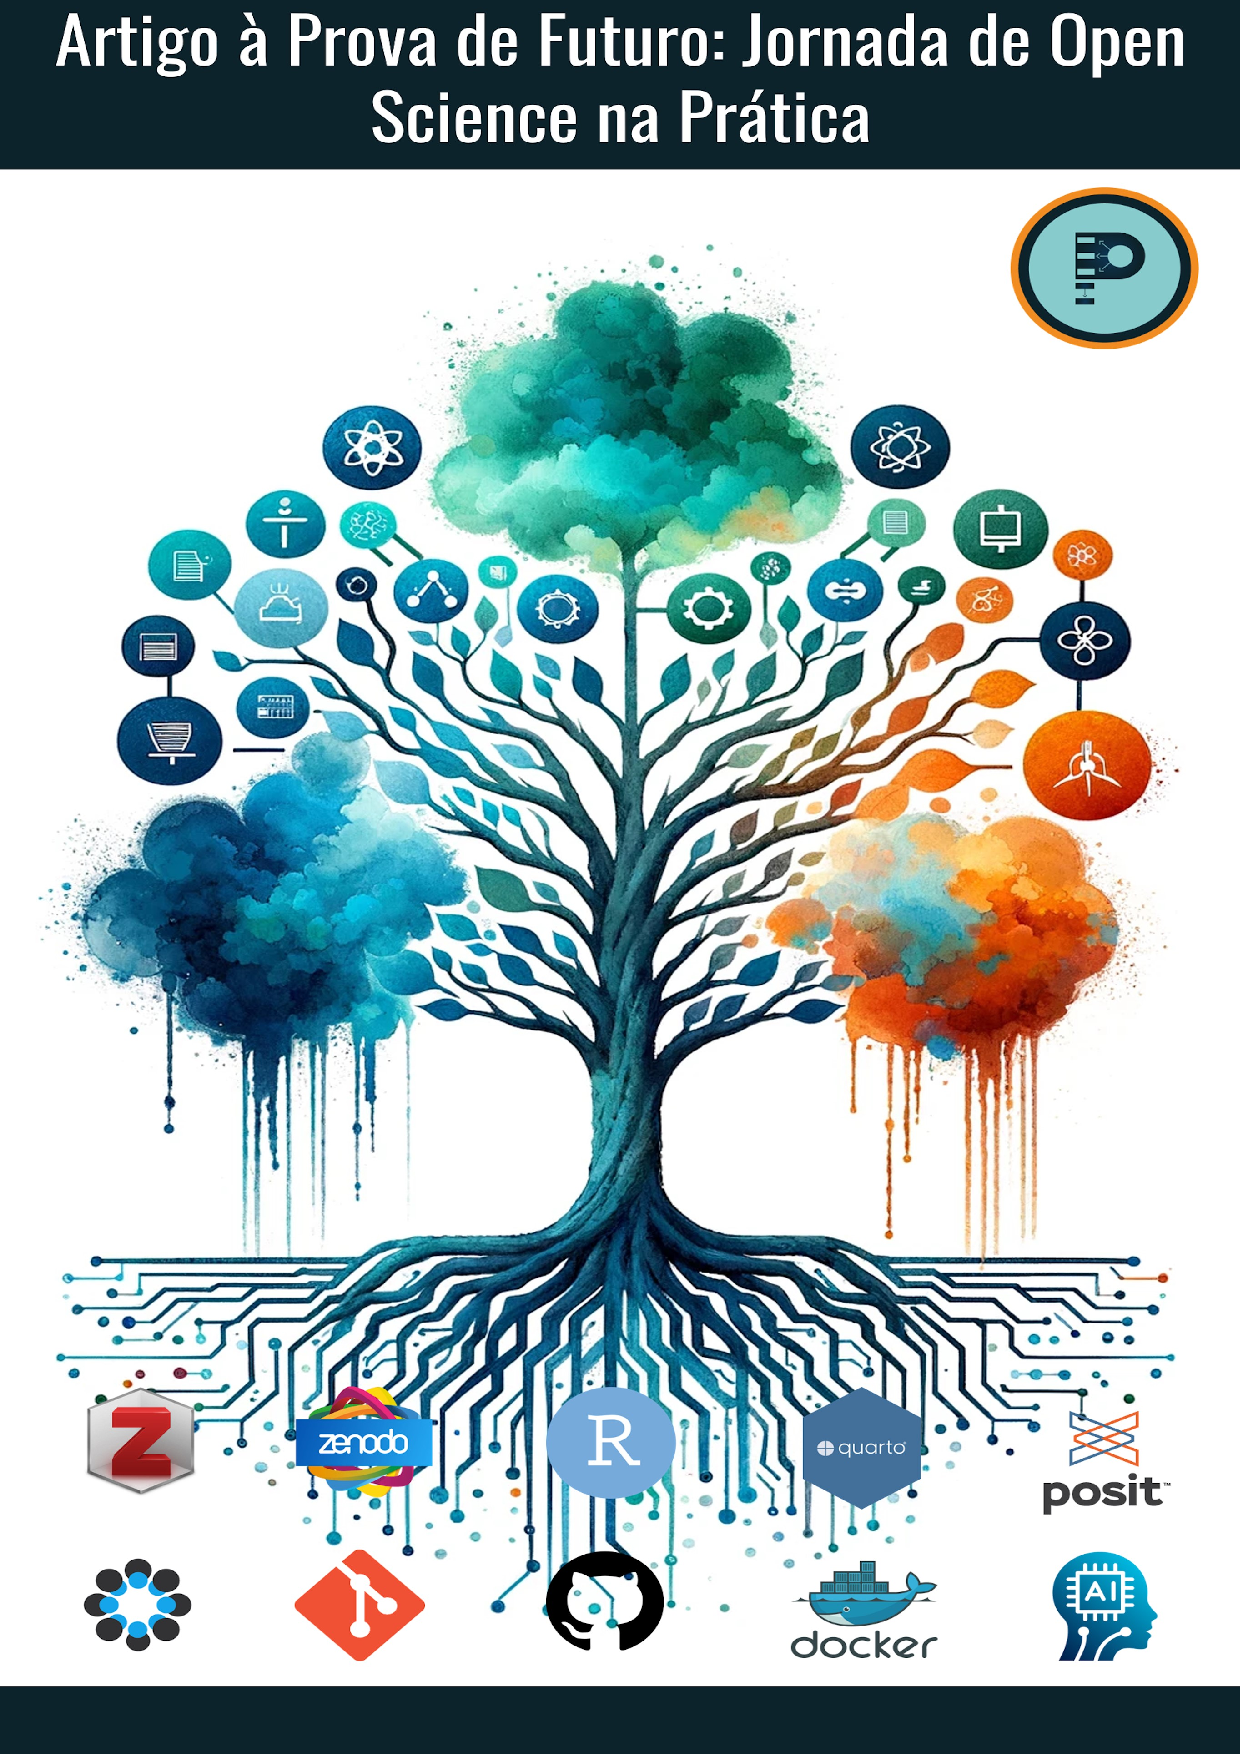
\includepdf[fitpaper=true,pages=-]{img/cover-book}
\end{center}
\let\maketitle\oldmaketitle
\maketitle
\AtBeginShipoutNext{\AtBeginShipoutDiscard}
\mainmatter
%\pagestyle{plain}

\renewcommand*\contentsname{Índice}
{
\hypersetup{linkcolor=}
\setcounter{tocdepth}{2}
\tableofcontents
}
\mainmatter
\bookmarksetup{startatroot}

\chapter*{O Curso 🏢}\label{sec-home}
\addcontentsline{toc}{chapter}{O Curso 🏢}

\markboth{O Curso 🏢}{O Curso 🏢}

Página do curso \textbf{``Artigo à Prova de Futuro: Jornada de Open
Science na Prática''}. Aqui você encontrará informações sobre o programa
do curso, materiais para seu acompanhamento e sugestões de leituras
sobre a prática da ciência aberta (artigos, notas de aulas, blogs,
vídeos, etc.).

Caso você caiu nessa página por acaso, saiba que o poderá se inscrever
no curso \href{https://forms.gle/b6Zio7oL8XxxhhtS9}{aqui}: independente
se ele estiver acontecendo no momento, será convidado a participar da
próxima versão.

\section*{Sobre os instrutores}\label{sec-instrutor}

\markright{Sobre os instrutores}

O curso é coordenado e ministrado por Pablo Rogers, doutor em
administração pela Universidade de São Paulo (FEA/USP) e professor de
finanças e métodos quantitativos desde 2005. Em sua
\href{https://github.com/phdpablo}{página de perfil do Github} temos
informações de seus trabalhos recentes, e no seu
\href{https://phdpablo.com/}{site pessoal}, detalhes sobre suas
formações, competências, trajetória e projetos.

Na sua versão atual o curso também será ministrado por Ricardo Limongi,
doutor em administração pela Fundação Getúlio Vargas (FGV-SP) e
professor de marketing e métodos quantitativos desde 2008 e atual editor
chefe da Brazilian Administration Review (BAR). Em seu
\href{https://www.instagram.com/limongi/}{perfil do Instagram} é
possível acompanhar sua agenda de atividades, cursos e palestras sobre
inteligência artificial aplicada aos negócios e pesquisa. Em seu
\href{https://www.youtube.com/@ricardolimongi_ia}{canal do YouTube}, é
possível encontrar vídeos das suas atividades: congressos, palestras,
aulas, etc.

\section*{Objetivos}\label{sec-about}

\markright{Objetivos}

O curso tem objetivo de introduzir os conceitos relacionados com a
Ciência Aberta (CA) e a prática da pesquisa reprodutível. O curso aborda
temas introdutórios sobre CA, com foco no ferramental disponível para
tornar a pesquisa mais transparente, reprodutível e acessível. O curso é
voltado para pesquisadores e estudantes de pós-graduação, mas aberto a
qualquer pessoa interessada em aprender sobre a prática da CA. O
protagonista do curso é o pesquisador brasileiro que deseja aprimorar a
qualidade e a transparência de sua pesquisa, e que busca ferramentas
para tornar-lá mais eficiente e acessível.

Trata-se de um curso intermitente programado para acontecer em 4
encontros de 4 horas/aula (ou 8 encontros de 2 horas/aula), totalizando
16 horas/aula. Num primeiro momento, a ideia que o curso seja remoto e
síncrono para alcançar um número maior de interessados. Ele poderá
acontecer mais de uma vez no ano, com datas e horários a serem
definidos. Para o calendário atual do curso, consulte a seção
\href{https://phdpablo.github.io/curso-open-science/00-schedule.html}{Agenda}.

O curso é gratuito e com de certificado de extensão pela Universidade
Federal de Uberlândia (UFU). As inscrições são feitas por meio de um
\href{https://forms.gle/wRNWAU9Ffyp7o4Vq9}{formulário} intermediado pelo
projeto
\href{https://www.youtube.com/c/PsicoEconoMETRIA}{Psico\&Econo\_METRIA}.
Quando da previsão das datas, uma campanha de e-mail marketing divulgará
o link para a inscrição através de coordenações de pós-graduações
selecionadas.

As vagas são limitadas e a seleção será feita por ordem de inscrição.
Após o preenchimento das vagas, os demais interessados serão inscritos
automaticamente numa lista de espera e, tempestivamente, serão avisados
sobre a próxima edição do curso. Após selecionados, os inscritos
receberão um e-mail com instruções para acesso à plataforma de aulas
síncronas e para a realização das atividades prévias ao curso.

\section*{Ementa}\label{sec-ementa}

\markright{Ementa}

Introdução da Ciência Aberta / Repositórios da Ciência Aberta /
Gerenciamento de Referências e Bibliotecas / Gestão de Projetos, Dados e
Scripts / Controle de Versão / Documentos Reprodutíveis / Controle de
Ambiente / IA Aplicada à Pesquisa Científica.

\section*{Metodologia}\label{sec-method}

\markright{Metodologia}

Num primeiro momento, o curso foi concebido para acontecer de forma
remota e síncrona, com aulas expositivas e teóricas, porém em grande
medida, o conteúdo é essencialmente prático. Algumas aulas poderão ser
gravadas e disponibilizadas no
\href{https://www.youtube.com/c/PsicoEconoMETRIA}{canal do YouTube do
projeto Psico\&Econo\_METRIA}, mas a intenção é que o conteúdo principal
seja síncrono, para uma maior interação entre os participantes.

Nesse sentido, o material do curso organizado nesse site refere-se ao
roteiro estruturado (enrendo) de tudo que se vê nas aulas síncronas e
conteúdos adicionais (bibliografia, notas de aulas, links, etc).

A proposta do curso busca seguir de perto a mensagem de Dogucu \&
Çetinkaya-Rundel (2022). Nesse artigo as autoras abordam a importância
da reprodutibilidade na ciência de dados, tanto na pesquisa quanto no
ensino. Elas recomendam que os professores-pesquisadores adotem fluxos
de trabalho reprodutíveis em suas pesquisas e ensinem esses fluxos de
trabalho aos seus alunos. Elas propõem uma dimensão para as práticas de
reprodutibilidade, focada exclusivamente nas ferramentas para o ensino
(todos os materiais de ensino devem ser computacionalmente
reprodutíveis, bem documentados e abertos).

\newpage

\section*{Citação}\label{sec-cite}

\markright{Citação}

Se você utilizar o material desse curso em algum trabalho acadêmico, por
favor, cite o livro do curso da seguinte forma:

\begin{tcolorbox}[enhanced jigsaw, breakable, left=2mm, opacityback=0, bottomrule=.15mm, arc=.35mm, colback=white, colframe=quarto-callout-important-color-frame, rightrule=.15mm, toprule=.15mm, leftrule=.75mm]

Rogers, P. (2024). Artigo à Prova de Futuro: Jornada de Open Science na
Prática (1.0). Disponível em:
https://phdpablo.github.io/curso-open-science/.
https://doi.org/10.5281/zenodo.12593928

\end{tcolorbox}

BibTex:

\begin{Shaded}
\begin{Highlighting}[]
\SpecialCharTok{@}\NormalTok{misc\{rogers2024,}
\NormalTok{  author       }\OtherTok{=}\NormalTok{ \{Rogers, Pablo\},}
\NormalTok{  title        }\OtherTok{=}\NormalTok{ \{\{Artigo à Prova de Futuro}\SpecialCharTok{:}\NormalTok{ Jornada de Open Science }
\NormalTok{                   na Prática\}\},}
\NormalTok{  month        }\OtherTok{=}\NormalTok{ jun,}
\NormalTok{  year         }\OtherTok{=} \DecValTok{2024}\NormalTok{,}
\NormalTok{  publisher    }\OtherTok{=}\NormalTok{ \{Zenodo\},}
\NormalTok{  version      }\OtherTok{=}\NormalTok{ \{}\FloatTok{1.0}\NormalTok{\},}
\NormalTok{  doi          }\OtherTok{=}\NormalTok{ \{}\FloatTok{10.5281}\SpecialCharTok{/}\NormalTok{zenodo}\FloatTok{.12593928}\NormalTok{\},}
\NormalTok{  url          }\OtherTok{=}\NormalTok{ \{https}\SpecialCharTok{:}\ErrorTok{//}\NormalTok{phdpablo.github.io}\SpecialCharTok{/}\NormalTok{curso}\SpecialCharTok{{-}}\NormalTok{open}\SpecialCharTok{{-}}\NormalTok{science}\SpecialCharTok{/}\NormalTok{\}}
\NormalTok{\}}
\end{Highlighting}
\end{Shaded}

\section*{Licença}\label{licenuxe7a}

\markright{Licença}

Artigo à Prova de Futuro: Jornada de Open Science na Prática by Pablo
Rogers is licensed under CC BY-NC-SA 4.0

\bookmarksetup{startatroot}

\chapter*{Pré-requisitos 📇}\label{sec-prework}
\addcontentsline{toc}{chapter}{Pré-requisitos 📇}

\markboth{Pré-requisitos 📇}{Pré-requisitos 📇}

O curso não exige conhecimento prévio em programação, mas é recomendável
que o aluno tenha familiaridade com o uso de computadores (ambiente
Windows) e com a escrita de textos científicos. Nesse sentido, não é
necessário ter conhecimento prévio sobre as ferramentas e plataformas
que utilizaremos no curso: Zotero, OSF, Zenodo, Git, Github, RStudio,
Quarto/RMarkdown, Docker, etc; mas desejável que o aluno já as tenha
instalado e/ou cadastro nas plataformas.

Abaixo descrevemos sucintamente o que é cada uma dessas ferramentas e
plataformas, e como você pode se preparar para o curso. Também
apresentamos um vídeo curto sobre a instalação e cadastro em cada uma
delas. A ideia é que você já tenha todas as ferramentas e plataformas
instaladas e/ou cadastro antes do início do curso, para que possamos
focar no conteúdo e prática durante as aulas síncronas. Mas pode ficar
tranquilo, pois na primeira aula do curso abordaremos essas tarefas, e
caso ainda haja alguma dúvida na instalação e cadastro, dedicaremos
algum tempo para saná-las.

Outras soluções que iremos discutir e testar durante o curso, como
alguns pacotes do R, e aplicações de IA no último módulo, deixaremos
para as aulas remotas. Essas soluções na sua maioria requerem cadastros
rápidos, e podem ser feitos de forma instantânea via conta
Google/Microsoft/Apple.

\begin{tcolorbox}[enhanced jigsaw, opacitybacktitle=0.6, titlerule=0mm, left=2mm, toptitle=1mm, opacityback=0, arc=.35mm, colback=white, rightrule=.15mm, breakable, leftrule=.75mm, bottomrule=.15mm, colbacktitle=quarto-callout-important-color!10!white, colframe=quarto-callout-important-color-frame, coltitle=black, bottomtitle=1mm, toprule=.15mm, title=\textcolor{quarto-callout-important-color}{\faExclamation}\hspace{0.5em}{Tip \ref*{tip-prompt}: ChatGPT para suas notas de leituras}]

\quartocallouttip{tip-prompt} 

Os resumos das bibliografias que apresentamos em cada uma das seções
foram elaborados com o auxílio do ChatGPT 4, seja pelo o
\href{https://chat.openai.com/}{webapp da OpenAI} ou pelo
\href{https://copilot.microsoft.com/}{Copilot} (ou buscador Bing) da
Microsoft.\vspace{0.5em}

Destacamos (selecionamos através de marca texto no Zotero, por exemplo)
as passagens que consideramos importante do artigo científico, tendo em
vista a perspectiva e fins no momento da leitura, e posteriormente se
copia e cola as notas de leitura com a seguinte prompt:\vspace{0.5em}

``\emph{Senteces in the text are reading notes, that is, what I found
most important and interesting, from a scientific article on the topic
open science. I would like you to summarize the notes in a descriptive
text and concatenate the arguments highlighted in the notes. Give your
answer in Portuguese}''

\end{tcolorbox}

\begin{tcolorbox}[enhanced jigsaw, opacitybacktitle=0.6, titlerule=0mm, left=2mm, toptitle=1mm, opacityback=0, arc=.35mm, colback=white, rightrule=.15mm, breakable, leftrule=.75mm, bottomrule=.15mm, colbacktitle=quarto-callout-caution-color!10!white, colframe=quarto-callout-caution-color-frame, coltitle=black, bottomtitle=1mm, toprule=.15mm, title=\textcolor{quarto-callout-caution-color}{\faFire}\hspace{0.5em}{Não confie cegamente na IA}]

Você simplesmente copia e cola os resultados do ChatGPT para compilar
essas notas de leituras? Não. Após o resultado do ChatGPT você deve
revisar o sumário das notas de leituras e fazer ajustes, que somente são
possíveis porque leu o artigo por completo. A despeito do ChatGPT fazer
um bom serviço nesse sentido, ele ainda comete muitos deslizes. Deslizes
esses que você não pode deixar passar num texto científico, e somente
captaria a partir da leitura do artigo ou sendo conhecedor do assunto
abordado.

\end{tcolorbox}

\begin{tcolorbox}[enhanced jigsaw, opacitybacktitle=0.6, titlerule=0mm, left=2mm, toptitle=1mm, opacityback=0, arc=.35mm, colback=white, rightrule=.15mm, breakable, leftrule=.75mm, bottomrule=.15mm, colbacktitle=quarto-callout-note-color!10!white, colframe=quarto-callout-note-color-frame, coltitle=black, bottomtitle=1mm, toprule=.15mm, title=\textcolor{quarto-callout-note-color}{\faInfo}\hspace{0.5em}{Outra curiosidade\ldots{}}]

A
\href{https://phdpablo.github.io/curso-open-science/img/cover.png}{imagem
cover desse curso} foi gerada por uma IA, com posteriores ajustes (off
course!). Existem diversos geradores de imagens que você pode testar
gratuitamente, mas eu costumo utilizar o i)
\href{https://openai.com/dall-e/}{DALL-E}, que é uma solução da OpenAI
que também pode ser utilizada no
\href{https://copilot.microsoft.com/}{Copilot da Microsoft}; ii) o
\href{https://playgroundai.com/}{PlaygroundAI}, e iii) o
\href{https://gemini.google.com/app}{Gemini} do Google.

\end{tcolorbox}

\section*{Github}\label{sec-githubprework}
\addcontentsline{toc}{section}{Github}

\markright{Github}

Primeiramente, se cadastre no Github: \url{https://github.com/signup},
pois com ele você poderá acessar o material do curso e interagir com os
demais participantes. E com a conta do Github você também poderá se
cadastrar em outras plataformas, como o Zenodo, OSF, etc. Algumas
features que aprenderemos no curso exigem o vínculo entre as contas. Se
for professor ou estudante, você pode solicitar o
\href{https://education.github.com/}{GitHub Education} e ter acesso, por
exemplo, ao Copilot, uma das ferramentas de IA mais interessante. Por
isso, é importante que você se cadastre com um e-mail institucional. Use
o mesmo e-mail para se cadastrar em todas plataformas.

\url{https://youtu.be/Nmjh9KsV6eU}

\section*{Git}\label{sec-gitprework}
\addcontentsline{toc}{section}{Git}

\markright{Git}

Github não é a mesma coisa que Git. O Github é uma plataforma, e o Git é
uma ferramenta. Instale a versão mais recente do Git:
\url{https://git-scm.com/downloads}. O Git é uma ferramenta de controle
de versão, e o Github é uma plataforma que utiliza o Git. O Git é uma
ferramenta essencial para a prática da CA, e é uma das ferramentas mais
importantes para o pesquisador que deseja tornar sua pesquisa mais
transparente e reprodutível.

\url{https://youtu.be/XCa6mE0bEI0}

\section*{Zotero}\label{sec-zoteroprework}
\addcontentsline{toc}{section}{Zotero}

\markright{Zotero}

Baixe a versão mais recente do Zotero:
\url{https://www.zotero.org/download/} e cadastre uma conta:
\url{https://www.zotero.org/user/register/}. Vamos discutir sobre o
Zotero e diversos plugins que são úteis no dia-a-dia do pesquisador.
Atualmente, o Zotero é a ferramenta mais completa para gerenciamento de
referências e bibliotecas, e se integra nativamente com o RStudio e
diversas ferramentas de IA.

\url{https://youtu.be/ZSFq6LHaDJ4}

\section*{OSF}\label{sec-osfprework}
\addcontentsline{toc}{section}{OSF}

\markright{OSF}

Cadastre no Open Science Framework (OSF):
\url{https://osf.io/register/}. Como veremos, essa plataforma é uma das
mais importantes para a prática da CA. Ela está no começo (pré-registro)
e no final (repositório de dados e pré-print) do ciclo de vida
(workflow) de um projeto de pesquisa.

\url{https://youtu.be/WQ4O-8O6MwI}

\section*{Zenodo}\label{sec-zenodoprework}
\addcontentsline{toc}{section}{Zenodo}

\markright{Zenodo}

Apesar do Zenodo cumprir funções similares ao OSF e até mesmo ao Github,
ele é mais voltado para a publicação de dados e publicações científicas
pontuais. Cadastre no Zenodo: \url{https://zenodo.org/login/} e víncule
sua conta com o Github. Isso será útil, principalmente, para geração de
DOI de repositórios do Github.

\url{https://youtu.be/pZaqL3Auxb0}

\section*{RStudio}\label{sec-rstudioprework}
\addcontentsline{toc}{section}{RStudio}

\markright{RStudio}

Baixe a versão mais recente do RStudio:
\url{https://posit.co/download/rstudio-desktop/}. O RStudio é uma
Integrated Development Environment (IDE) para a linguagem R. O RStudio é
uma ferramenta essencial para a prática da CA em R, pois integra as
principais soluções que abordaremos no curso (Zotero, Quarto,
Git/Github, etc.). A empresa RStudio recentemente mudou o nome para
Posit, com o objetivo refletir melhor a expansão da empresa para além do
desenvolvimento de ferramentas para R, incluindo Python e outras
linguagens. Nesse mesmo link você pode baixar o R, que é a linguagem de
programação que utilizaremos no curso.

\url{https://youtu.be/KM2jxaNIEUk}

\section*{Quarto}\label{sec-quartoprework}
\addcontentsline{toc}{section}{Quarto}

\markright{Quarto}

Baixe a versão mais recente do Quarto CLI (Command Line Interface):
\url{https://www.quarto.org/}. O Quarto é uma linguagem de marcação que
permite a criação de documentos reprodutíveis e dinâmicos. Ele é uma
evolução e tende a substituir o RMarkdown, que é a principal linguagem
de marcação do R. O Quarto engloba e adiciona diversas outras vantagens
ao RMarkdown, tal como a possibilidade de criar documentos reprodutíveis
em Python, Julia, etc. Se você já tem algum conhecimento de RMarkdown,
não se preocupe, pois o Quarto é uma extensão natural.

\url{https://youtu.be/-HvOMVkk6I4}

\section*{Docker}\label{sec-dockerprework}
\addcontentsline{toc}{section}{Docker}

\markright{Docker}

Baixe a versão mais recente do Docker:
\url{https://www.docker.com/products/docker-desktop}. Nesse mesmo link
você cria uma conta. O Docker é uma plataforma para desenvolvimento,
envio e execução de aplicativos. O Docker é uma ferramenta essencial
para a prática da CA, pois permite a criação de ambientes reprodutíveis.

\url{https://youtu.be/WjXQxhTLlrQ}

\bookmarksetup{startatroot}

\chapter*{Agenda 📅}\label{sec-schedule}

\markboth{Agenda 📅}{Agenda 📅}

Planejamento dos dias (📅) e horários das aulas (⏲️), conforme a ementa
do curso. Na seção de cada uma das aulas temos materiais adicionais para
o respectivo conteúdo. Quando disponível, por aqui, poderás acessar os
slides utilizados nas aulas (🗣️), aulas gravadas ou indicações de vídeo
(🎥)\footnote{Na primeira edição do curso a equipe organizadora decidiu
  não publicar as aulas. Elas estarão disponíveis apenas privativamente
  para os inscritos no curso, através da platorma de reuniões adotada
  (Microsoft Teams). No futuro, quando o coordenador considerar que o
  curso esteja efetivamente formatado, as aulas gravadas serão
  publicadas no canal
  \href{https://www.youtube.com/c/PsicoEconoMETRIA}{Psico\&Econo\_METRIA}}
e leituras básica sobre os conteúdos (📓).

\begin{longtable}[]{@{}
  >{\raggedright\arraybackslash}p{(\columnwidth - 6\tabcolsep) * \real{0.0600}}
  >{\centering\arraybackslash}p{(\columnwidth - 6\tabcolsep) * \real{0.0760}}
  >{\centering\arraybackslash}p{(\columnwidth - 6\tabcolsep) * \real{0.7960}}
  >{\centering\arraybackslash}p{(\columnwidth - 6\tabcolsep) * \real{0.0680}}@{}}
\toprule\noalign{}
\begin{minipage}[b]{\linewidth}\raggedright
Aula/Conteúdo
\end{minipage} & \begin{minipage}[b]{\linewidth}\centering
Data
\end{minipage} & \begin{minipage}[b]{\linewidth}\centering
Material Principal
\end{minipage} & \begin{minipage}[b]{\linewidth}\centering
Instrutor
\end{minipage} \\
\midrule\noalign{}
\endhead
\bottomrule\noalign{}
\endlastfoot
Capítulo~\ref{sec-intro} & 📅04/06/24⏲️19:00 &
\href{./resources/01-intro.pdf}{🗣}\href{https://www.youtube.com/live/7ewEcTATkZM?si=Lq40IAoDgsy_A619}{🎥}\href{https://doi.org/10.1590/S0034-759020230408}{📓}
& Ricardo Limongi \\
Capítulo~\ref{sec-osf} & 📅06/06/24⏲️19:00 &
\href{https://osf.io/wm8vs}{🗣️}\href{https://www.youtube.com/watch?v=B19MPDJX_vs}{🎥}\href{https://doi.org/10.1002/cpet.32}{📓}
& Pablo Rogers \\
Capítulo~\ref{sec-zotero} & 📅11/06/24⏲️19:00 &
\href{https://osf.io/emxz8}{🗣️}\href{https://youtu.be/tnbwKj6-pD8?si=Yx9IC2LhrplvA6g1}{🎥}\href{https://kuscholarworks.ku.edu/handle/1808/34983}{📓}
& Pablo Rogers \\
Capítulo~\ref{sec-project} & 📅13/06/24⏲️19:00 &
\href{./resources/04-project.pdf}{🗣️}\href{https://youtu.be/l8yh3f8Tbv8?si=Yeq-xRxmffF7S1dk}{🎥}\href{https://doi.org/10.1371/journal.pcbi.1005510}{📓}
& Pablo Rogers \\
Capítulo~\ref{sec-git} & 📅18/06/24⏲️19:00 &
\href{./resources/05-git.pdf}{🗣️}\href{https://youtu.be/uQL6NOSd9cc?si=TIYenlvIzKpoQ2dQ&t=1775}{🎥}\href{https://doi.org/10.1177/2515245918754826}{📓}
& Pablo Rogers \\
Capítulo~\ref{sec-quarto} & 📅20/06/24⏲️19:00 &
\href{https://tracykteal.quarto.pub/intro-to-quarto/}{🗣️}\href{https://youtu.be/XuxyzBhDvLg?si=iRCnXPJkmqbLuFty&t=1469}{🎥}\href{https://doi.org/10.31219/osf.io/ur4xn}{📓}
& Pablo Rogers \\
Capítulo~\ref{sec-docker} & 📅25/06/24⏲️19:00 &
\href{https://kevinushey-2020-rstudio-conf.netlify.app/slides.html\#1}{🗣️}\href{https://youtu.be/N2STULZ1dYo?si=LAxCXfI9J0irxADD&t=523}{🎥}\href{https://doi.org/10.1177/25152459211017853}{📓}
& Pablo Rogers \\
Capítulo~\ref{sec-AI} & 📅27/06/24⏲️19:00 &
\href{https://admkt.face.ufg.br/p/49240-uso-de-ia-na-pesquisa-cientifica}{🗣️}\href{https://www.youtube.com/playlist?list=PL8Norrhzu5QZA9ODYlmW2NtPhD7YL6Z3j}{🎥}\href{https://doi.org/10.1590/1678-98732432e008}{📓}
& Ricardo Limongi \\
\end{longtable}

\bookmarksetup{startatroot}

\chapter{Introdução à Ciência Aberta}\label{sec-intro}

A pesquisa científica atual\footnote{O texto apresentado nessa seção é
  uma compilação de fragmentos do Projeto APQ-01225-24 submetido ao
  Edital Nº 001/2024 - Demanda Universal, da FAPEMIG, ainda em análise.
  O detalhamento desse projeto, quando se tornar público, poderá ser
  acompanhado no \href{http://osf.io/dnrgf}{OSF}: Rogers, P., Limongi,
  R., \& Barboza, F. (2024, May 29). The Practice of Open Science in
  Brazil. Retrieved from osf.io/dnrgf} enfrenta vários desafios (Munafò
et al., 2017). Problemas como o pequeno tamanho da amostra, pequenos
tamanhos de efeito, p-hacking e HARKing (viés positivo de publicação),
conflitos de interesse e a competição entre cientistas que trabalham
isoladamente sem combinar seus esforços, têm sido apontados como
catalizadores do que se convencionou chamar de ``crise de
reprodutibilidade'' na ciência (M. Baker, 2016; Munafò et al., 2017).

Pesquisas apontam que mais de 70\% de pesquisadores que tentaram,
falharam em reproduzir os experimentos de outros cientistas, e mais da
metade falhou em reproduzir seus próprios experimentos (M. Baker, 2016),
com estimativa de que 85\% dos esforços de pesquisas estejam sendo
desperdiçados (Munafò et al., 2017), gerando custos econômicos
bilionários (Freedman et al., 2015).

A despeito daqueles que advogam que não existe essa tal ``crise de
reprodutibilidade'' (Bernard, 2023; Fanelli, 2018; Protzko et al.,
2023), a grande maioria da comunidade científica concorda com sua
existência e defende a melhoria da transparência, reprodutibilidade e
eficiência na ciência (M. Baker, 2016).

Nesse contexto, o movimento da Ciência Aberta (CA) tem ganhado
notoriedade e mudado a percepção sobre o cenário científico global
(Crüwell et al., 2019). Ele busca tornar o conhecimento científico mais
acessível, transparente e colaborativo. Se apresenta como uma coleção de
práticas de democratização do conhecimento e ruptura com o formato único
de divulgação do conhecimento científico (Crüwell et al., 2019; Heinz \&
Miranda, 2024; Munafò et al., 2017). Ele surge do embate entre aqueles
que buscam compartilhar o conhecimento e aqueles que defendem mecanismos
de apropriação privada para a produção científica (Heinz \& Miranda,
2024).

A CA é um termo múltiplo e genérico (Vicente-Saez \& Martinez-Fuentes,
2018), que representa diversas interpretações, e é considerada um novo
modelo de divulgação e produção de resultados científicos por meio do
acesso livre e irrestrito ao conhecimento (Heinz \& Miranda, 2024). A CA
não é apenas um conceito, mas uma prática multifacetada que influencia o
ciclo de vida da pesquisa, desde a concepção até a disseminação dos
resultados (Silva \& Silveira, 2019).

Existem pelo menos cinco escolas de pensamento dentro da CA. Estas
escolas abrangem desde a arquitetura tecnológica necessária para
suportar a ciência até a inclusão do público geral na criação de
conhecimento, passando pela medição do impacto alternativo, acesso ao
conhecimento como um direito humano, e a pesquisa colaborativa como
inovação aberta (Silva \& Silveira, 2019).

A taxonomia proposta pela
\href{https://www.fosteropenscience.eu/foster-taxonomy/open-workflow-tools}{FOSTER}
(Facilitate Open Science Training for Eurpean Research), e sua releitura
revisada e ampliada para o contexto latino americano por Silveira et al.
(2023), tendo em vista as recomendações da UNESCO (2021), nos dá uma
dimensão da complexidade do assunto (vide ilustração em:
\url{https://doi.org/10.5281/zenodo.7836884}).

Existem vários argumentos que sustentam a importância da CA (Heinz \&
Miranda, 2024). Primeiramente, a CA pode trazer benefícios sociais
significativos, pois contribui para o avanço do conhecimento, a
inovação, a educação, a transparência e a participação cidadã. Além
disso, a CA pode trazer benefícios científicos ao aumentar a qualidade,
a reprodutibilidade, a eficiência e o impacto da pesquisa científica.
Ela também facilita a colaboração, a comunicação e a
interdisciplinaridade entre os pesquisadores. Por fim, a CA pode trazer
benefícios éticos ao promover a integridade, a responsabilidade, a
equidade e a diversidade na ciência, além de respeitar os direitos dos
autores, dos participantes e da sociedade como um todo.

Esses argumentos são fundamentais para legitimar a CA e destacar sua
importância no mundo atual (Heinz \& Miranda, 2024), principalmente,
como potencial transformador para reduzir desigualdades existentes em
tecnologias de informação e comunicação -- reduzir exclusões digitais,
tecnológicas e de conhecimento --, e acelerar o progresso rumo à
implementação da Agenda 2030 e realização dos Objetivos de
Desenvolvimento Sustentável (UNESCO, 2021).

O movimento da CA no Brasil está em uma fase transitória (Rezende \&
Falgueras, 2020) -- ainda consolidando o acesso aberto -- com o governo
desempenhando um papel crucial nesse processo. O Brasil tem ganhado
destaque por sua abordagem única na implementação da CA. Esta abordagem
é moldada por marcos regulatórios que se estendem desde o governo até as
instituições e agências de financiamento. Os regulamentos brasileiros,
particularmente aqueles que promovem a abertura de dados governamentais,
têm um impacto direto na prática científica. Eles incentivam a
transparência e facilitam o acesso a dados científicos originados de
instituições públicas (Rezende \& Falgueras, 2020).

A trajetória brasileira rumo à CA inicia com a abertura de dados na
esfera governamental entre 2009 e 2016, evoluindo para a criação de um
grupo de trabalho em 2017 pelo Ministério da Ciência, Tecnologia,
Inovações e Comunicações (MCTIC) para desenvolver uma política nacional
para a CA. Este esforço concentrou ênfase no reconhecimento dos dados de
pesquisa como ativos de desenvolvimento científico, econômico e social,
buscando facilitar seu acesso, compartilhamento e reutilização (Rezende
\& Falgueras, 2020).

Talvez por esse motivo, as políticas institucionais brasileiras revelam
um cenário ainda muito influenciado pela ``via verde'' do movimento de
acesso aberto, caracterizado pelo depósito de dados em repositórios
digitais abertos, e que o comprometimento efetivo do Brasil com a CA
ainda é incipiente. As regulamentações atuais favorecem principalmente o
acesso aberto, sem abordar de maneira abrangente outros aspectos da CA
(Rezende \& Falgueras, 2020). O Brasil é um dos líderes mundiais no
fornecimento de acesso universal às suas pesquisas e estudos (Neto et
al., 2016), com crescimento estável de sua produção científica
disponível em acesso aberto, principalmente, as áreas de Agricultura e
Ciência \& Tecnologia (Caballero-Rivero et al., 2019).

Em termos de pesquisa acadêmica sobre o tema no Brasil, os estudos são
precoces e concentrados na área de Ciência da Informação (Albano et al.,
2023). A despeito da maturidade da CA no Brasil, a importância do tema
-- materializada na quantidade de produção acadêmica -- tem aumentado
vertiginosamente (Albano et al., 2023), e a dispersão de autores e
respectivas instituições que publicam sobre o assunto, parece ser a
situação predominante.

Apesar de importantes atores nacionais, tais como CAPES, CNPq e Scielo,
defenderem o crescimento de iniciativas de CA (Mendes-Da-Silva, 2023), o
assunto no Brasil parece estar circunscrito em iniciativas de
importantes periódicos nacionais sobre dados aberto, capitaneados pelas
orientações da Scielo. Não foi encontrada nenhuma pesquisa empírica,
sobre a prática da CA no Brasil.

Por prática de CA entende-se a perspectiva micro da CA, relacionadas com
as terminologias e conhecimento em torno do fluxo de trabalho do gerador
de conhecimento científico aberto (Figura~\ref{fig-ca-micro}), ou seja,
o cientista que se propõe tornar sua pesquisa transparente, reprodutível
e replicável.

\begin{figure}

\href{https://doi.org/10.5281/zenodo.10835001}{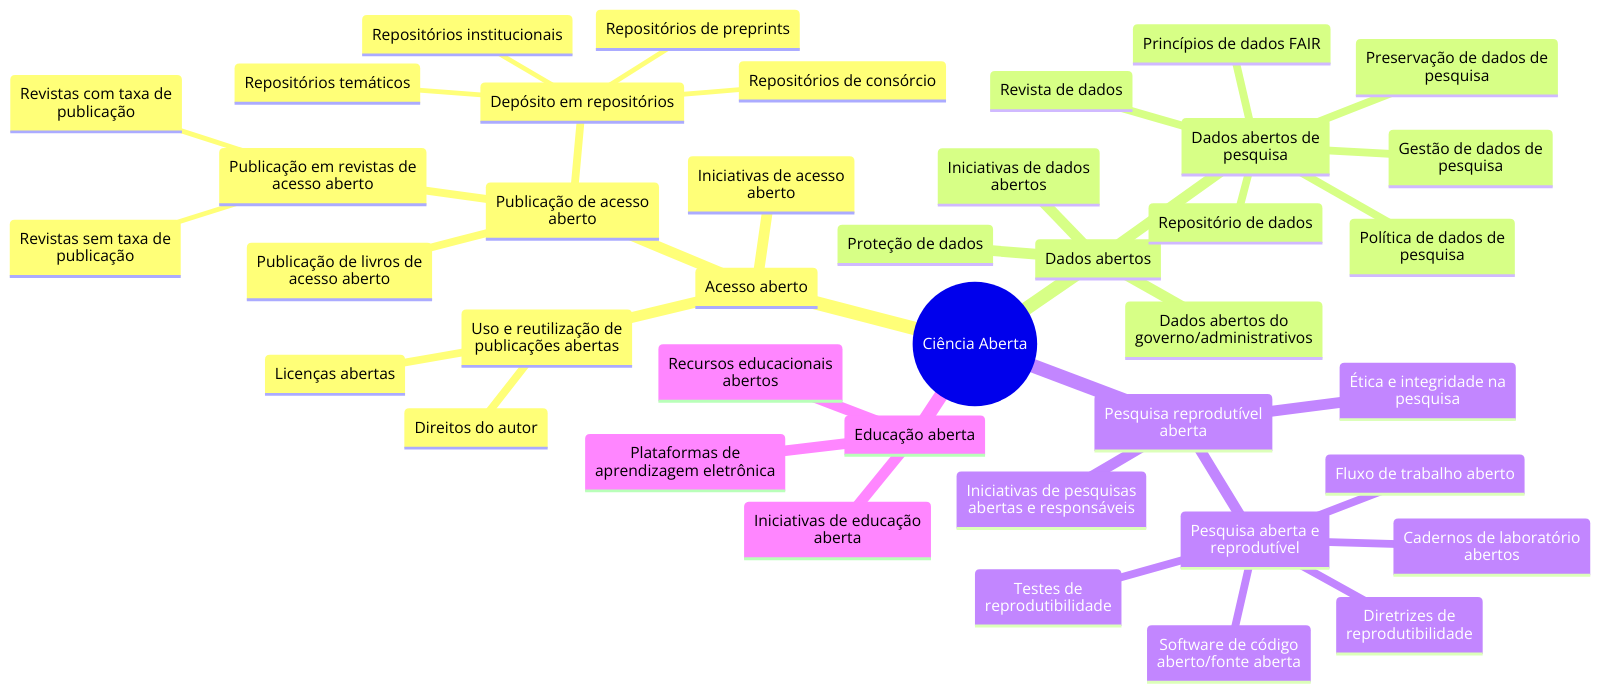
\includegraphics{img/ca-micro.png}}

\caption{\label{fig-ca-micro}Perspectiva micro da CA. Taxonomia
relacionada com terminologias e conhecimento em torno da prática (fluxo
de trabalho) do gerador de conhecimento científico aberto. Ilustração
disponível em: https://doi.org/10.5281/zenodo.10835001.}

\end{figure}%

Exclui-se a perspectiva macro, relacionadas com as ramificações
conceituais da CA concernentes às políticas públicas, infraestrutura,
envolvimento aberto de atores sociais e diálogo aberto com outros
sistemas de conhecimento (Figura~\ref{fig-ca-macro}). Essa última
perspectiva está fora do escopo da discussão do curso, que se concentra
em algumas das dimensões da perspectiva micro, particularmente, as
ferramentas disponíveis para compilação dos produtos científicos que
integram a publicação científica (UNESCO, 2021).

\begin{figure}

\href{https://doi.org/10.5281/zenodo.10835001}{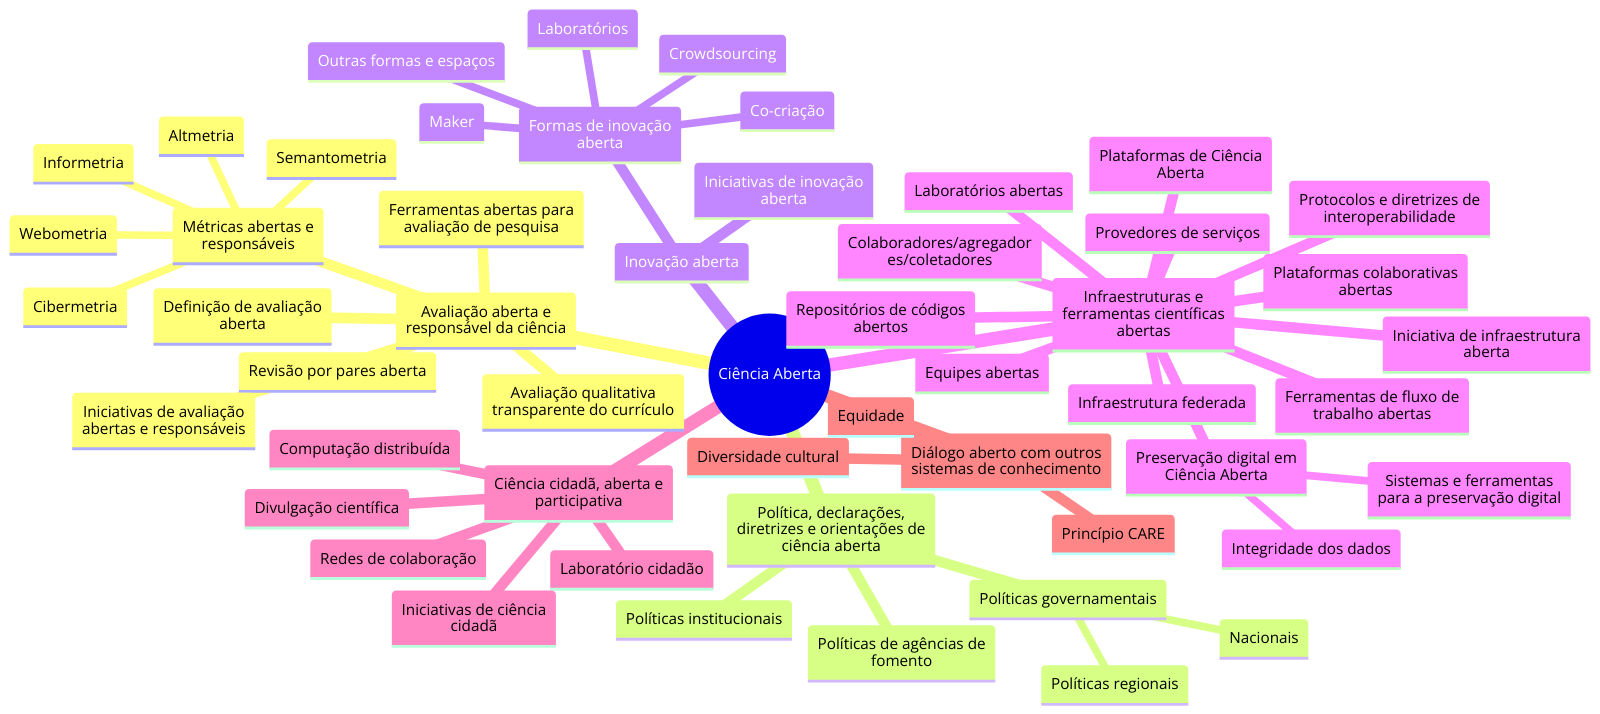
\includegraphics{img/ca-macro.png}}

\caption{\label{fig-ca-macro}Perspectiva macro da CA. Taxonomia
relacionada com as ramificações conceituais da CA concernentes às
políticas (públicas), infraestrutura, envolvimento aberto de atores
sociais (sociedade) e diálogo aberto com outros sistemas de
conhecimento. Ilustração disponível em:
https://doi.org/10.5281/zenodo.10835001}

\end{figure}%

Apesar de uma verossímil expectativa desabonadora, tendo em vista o
contexto da CA no Brasil, o diagnóstico da situação da prática da CA se
mostra importante, \emph{per si}, pois:

\begin{enumerate}
\def\labelenumi{\arabic{enumi}.}
\item
  ajuda a compreender a natureza exata do problema, suas causas, efeitos
  e riscos;
\item
  auxilia a alocação eficiente de recursos pelos atores envolvidos
  (e.g., os programas de pós-graduação podem direcionar os recursos para
  onde eles são mais necessários e onde terão o maior impacto;
\item
  orienta indicadores de desempenho e metas realistas, o que facilita a
  avaliação do progresso e a eficácia das ações tomadas;
\item
  permite que os atores envolvidos aprendam com os problemas
  enfrentados, adaptando-se e melhorando suas estratégias e processos
  para o futuro; e
\item
  torna possível desenvolver soluções ou intervenções que sejam
  diretamente direcionadas ao problema em questão, aumentando as chances
  de sucesso.
\end{enumerate}

Sobre esse último ponto, até para aqueles que não reconhecem a ``crise
de reprodutibilidade'' na ciência (Bernard, 2023), a comunidade
científica e atores importantes do cenário advogam que a solução inclui
educar os estudantes e pesquisadores desde cedo em todas as questões da
CA (D. H. Baker et al., 2023; Bezjak et al., 2018; Chopik et al., 2018;
Crüwell et al., 2019; Dogucu \& Çetinkaya-Rundel, 2022; Janz, 2015;
McAleer et al., 2022; Munafò et al., 2017; Toelch \& Ostwald, 2018).

A referida crise não deriva de má conduta científica, mas principalmente
da confusão entre replicar conclusões, replicar resultados, falta de
educação em estatística, lógica científica, método científico,
alfabetização de dados, etc. Para combater essas questões é necessário
investir em educação e disseminação de boas práticas de investigação
para uma mudança de cultura (D. H. Baker et al., 2023; Bezjak et al.,
2018; Chopik et al., 2018; Crüwell et al., 2019; Dogucu \&
Çetinkaya-Rundel, 2022; Janz, 2015; McAleer et al., 2022; Munafò et al.,
2017; Toelch \& Ostwald, 2018).

Investir em recursos humanos, treinamento, educação, alfabetização
digital, capacitação sistemática e contínua, e fomentar uma cultura
científica de CA, têm sido apresentadas como algumas das principais
medidas simultâneas para superar o cenário atual (Committee on
Reproducibility and Replicability in Science et al., 2019; European
Commission. Directorate General for Research and Innovation., 2017;
UNESCO, 2021). A proposta do curso pode contribuir para a literatura da
CA no Brasil, pois pretende perseguir dois objetivos concomitantes: 1)
diagnosticar sua prática junto aos pesquisadores brasileiros; e 2)
promover o desenvolvimento de uma intervenção educacional sobre a
prática (workflow) e principais ferramentas para compilação dos produtos
científicos que integram uma publicação científica aberta.

\begin{tcolorbox}[enhanced jigsaw, opacitybacktitle=0.6, titlerule=0mm, left=2mm, toptitle=1mm, opacityback=0, arc=.35mm, colback=white, rightrule=.15mm, breakable, leftrule=.75mm, bottomrule=.15mm, colbacktitle=quarto-callout-note-color!10!white, colframe=quarto-callout-note-color-frame, coltitle=black, bottomtitle=1mm, toprule=.15mm, title=\textcolor{quarto-callout-note-color}{\faInfo}\hspace{0.5em}{\emph{A Pratical Guide for Transparency in Psychological Science}
(Tip~\ref{tip-prompt})}]

O artigo (Klein et al., 2018) é um guia prático para pesquisadores que
desejam compartilhar os produtos de sua pesquisa. Os autores argumentam
que as práticas de pesquisa transparentes são essenciais para melhorar a
credibilidade e a cumulatividade da ciência.\vspace{0.5em}

O artigo fornece recomendações específicas sobre como compartilhar os
seguintes produtos de pesquisa:\vspace{0.5em}

\begin{itemize}
\tightlist
\item
  Protocolo de estudo
\item
  Materiais
\item
  Dados e metadados
\item
  Procedimento de análise
\item
  Relatórios de pesquisa\vspace{0.5em}
\end{itemize}

As recomendações gerais dos autores são as seguintes:\vspace{0.5em}

\begin{itemize}
\item
  \textbf{Torne a transparência um padrão}: isso significa compartilhar
  o máximo possível de informações sobre sua pesquisa, desde o início do
  processo.
\item
  \textbf{Não deixe que o perfeito seja inimigo do bom}: mesmo que você
  não possa compartilhar todos os detalhes de sua pesquisa, compartilhar
  alguma coisa é melhor do que nada.
\item
  \textbf{Compartilhe e documente o que puder}: isso ajudará a garantir
  que sua pesquisa seja reproduzível e confiável.
\item
  \textbf{Comece cedo}: começar a compartilhar informações sobre sua
  pesquisa no início do processo pode ajudá-lo a evitar problemas e
  economizar tempo.\vspace{0.5em}
\end{itemize}

Os autores também discutem algumas preocupações comuns que os
pesquisadores têm sobre as práticas de pesquisa transparentes. Eles
argumentam que essas preocupações são geralmente infundadas e que as
práticas transparentes têm muitos benefícios.\vspace{0.5em}

Os principais benefícios das práticas de pesquisa transparentes
são:\vspace{0.5em}

\begin{itemize}
\item
  \textbf{Melhor credibilidade da pesquisa}: os pesquisadores
  transparentes são mais propensos a serem vistos como confiáveis e
  honestos.
\item
  \textbf{Maior cumulatividade da ciência}: os pesquisadores
  transparentes tornam mais fácil para outros pesquisadores construir
  sobre seu trabalho.
\item
  \textbf{Mais oportunidades de colaboração e financiamento}: os
  pesquisadores transparentes são mais propensos a serem convidados para
  colaborar com outros pesquisadores e a receber financiamento.
\item
  \textbf{Maior eficiência da pesquisa}: as práticas transparentes podem
  ajudar os pesquisadores a economizar tempo e recursos.\vspace{0.5em}
\end{itemize}

Em conclusão, o artigo fornece informações valiosas para pesquisadores
que desejam compartilhar os produtos de sua pesquisa. As recomendações
dos autores são baseadas em evidências e podem ajudar os pesquisadores a
melhorar a qualidade e a credibilidade de seu trabalho.

\end{tcolorbox}

\begin{tcolorbox}[enhanced jigsaw, opacitybacktitle=0.6, titlerule=0mm, left=2mm, toptitle=1mm, opacityback=0, arc=.35mm, colback=white, rightrule=.15mm, breakable, leftrule=.75mm, bottomrule=.15mm, colbacktitle=quarto-callout-note-color!10!white, colframe=quarto-callout-note-color-frame, coltitle=black, bottomtitle=1mm, toprule=.15mm, title=\textcolor{quarto-callout-note-color}{\faInfo}\hspace{0.5em}{\emph{Easing Into Open Science: A Guide for Graduate Students and Their
Advisors} (Tip~\ref{tip-prompt})}]

O artigo (Kathawalla et al., 2021) fornece um guia para ajudar
estudantes de pós-graduação e seus orientadores a se envolverem na
prática da ciência aberta (CA). A CA é descrita como um termo amplo que
se refere a uma variedade de princípios e comportamentos relacionados à
transparência, credibilidade, reprodutibilidade e
acessibilidade.\vspace{0.5em}

O artigo sugere oito práticas de CA (das quais destaco sete) que
estudantes de pós-graduação iniciantes podem começar a adotar hoje. Cada
comportamento é classificado em termos de dificuldade (fácil, médio,
difícil) e apresentado em ordem de adoção sugerida. Em cada prática,
eles seguem o formato de o quê, por quê, como e
preocupações.\vspace{0.5em}

Algumas das práticas sugeridas incluem:\vspace{0.5em}

\begin{enumerate}
\def\labelenumi{\arabic{enumi}.}
\item
  \textbf{Fluxo de Trabalho do Projeto (Nível Fácil)}: isso inclui a
  estrutura da pasta do arquivo, convenções de nomenclatura de
  documentos, controle de versão, armazenamento em nuvem e outros
  detalhes. Ter um sistema de fluxo de trabalho de projeto dedicado
  ajuda a manter sua pesquisa organizada, melhorando a
  reprodutibilidade, minimizando erros e facilitando colaborações com
  outros e com você no futuro.
\item
  \textbf{Preprints (Nível Fácil)}: postar um manuscrito antes de
  submetê-lo a uma revista permite um feedback mais amplo do que o que é
  proporcionado pela revisão por pares e pode ajudar a melhorar um
  artigo antes da submissão, identificando quaisquer falhas importantes.
\item
  \textbf{Código Reprodutível (Nível Médio)}: o código reprodutível para
  análise de dados e visualizações (por exemplo, tabelas, figuras)
  refere-se a uma versão detalhada e escrita do seu código que
  permitiria a outra pessoa (ou a você no futuro) gerar a mesma saída
  relatada em seu manuscrito.
\item
  \textbf{Compartilhamento de Dados (Nível Médio)}: compartilhar dados
  refere-se a tornar o conjunto de dados desidentificado usado para um
  projeto disponível para outros pesquisadores.
\item
  \textbf{Escrita de Manuscrito Transparente (Nível Médio)}: Para
  escrever um manuscrito transparente, claro e reprodutível, é útil
  seguir as diretrizes ou padrões de escrita de manuscritos.
\item
  \textbf{Pré-registro (Nível Médio)}: o pré-registro refere-se à
  postagem de um esboço cronometrado das perguntas de pesquisa,
  hipóteses, método e plano de análise para um projeto específico antes
  da coleta de dados e/ou análise.
\item
  \textbf{Relatório Registrado (Nível Difícil)}: os Relatórios
  Registrados envolvem um processo de submissão em duas partes, onde os
  autores primeiro enviam uma proposta de Estágio 1, que inclui a
  introdução, método e plano de análise - tudo antes que a coleta de
  dados e/ou análise tenha sido feita.\vspace{0.5em}
\end{enumerate}

O artigo enfatiza que se envolver em uma prática de CA é melhor do que
nenhuma e que a CA é apenas uma boa ciência. Além disso, sugere-se que
se construa sobre o trabalho que já foi feito em vez de reinventar a
roda. A maioria das práticas sugeridas se concentra no uso do
\href{https://osf.io}{Open Science Framework}.

\end{tcolorbox}

\bookmarksetup{startatroot}

\chapter{Repositórios da Ciência Aberta}\label{sec-osf}

No contexto da CA, existem diversos repositórios disponíveis, cada um
com suas funções e propósitos específicos. Esses repositórios são
essenciais para promover a transparência, acessibilidade e colaboração
na pesquisa científica. Eles assumem um papel crucial na democratização
do conhecimento e na promoção da colaboração científica. Cada qual com
suas particularidades, oferecem aos pesquisadores ferramentas para
armazenar, compartilhar e gerenciar dados, publicações e outros
materiais de pesquisa, ou se preferir, todo o ciclo de vida da pesquisa.

\begin{itemize}
\tightlist
\item
  \href{https://www.zenodo.org}{\textbf{Zenodo}}: é um repositório
  gerido pelo CERN em colaboração com o projeto
  \href{https://www.openaire.eu/}{OpenAIRE} da União Europeia. Oferece
  armazenamento gratuito e seguro para dados de pesquisa, com a
  capacidade de gerar DOIs para facilitar a citação dos dados.
\item
  \href{https://www.figshare.com}{\textbf{Figshare}}: é um repositório
  comercial que permite aos pesquisadores armazenar, compartilhar e
  descobrir dados de pesquisa. Oferece ferramentas para visualização de
  documentos, gráficos e outros tipos de dados diretamente no navegador,
  além de gerar DOIs para os projetos.
\item
  \href{https://data.mendeley.com}{\textbf{Mendeley Data}}: é um
  repositório de dados de pesquisa da Elsevier, permitindo o
  armazenamento, compartilhamento e citação de conjuntos de dados. Ele
  suporta uma ampla gama de tipos de dados e está integrado com a
  plataforma de referência Mendeley.
\item
  \href{https://dataverse.harvard.edu}{\textbf{Harvard Dataverse}}: é
  uma rede de repositórios que permite aos pesquisadores compartilhar,
  armazenar e citar dados de pesquisa. Ele oferece ferramentas avançadas
  para a gestão de dados, incluindo controle de versões e metadados
  ricos, essenciais para o gerenciamento do ciclo de vida da pesquisa.
\item
  \href{https://arxiv.org}{\textbf{arXiv}}: é um repositório de
  pré-impressões de artigos científicos em física, matemática, ciência
  da computação e outras áreas. Ele permite aos pesquisadores
  compartilhar seus trabalhos antes da revisão por pares, facilitando o
  acesso à pesquisa em estágios iniciais.
\item
  \href{https://github.com}{\textbf{Github}}: é uma plataforma de
  desenvolvimento colaborativo baseada em Git, amplamente utilizada por
  pesquisadores para compartilhar código, documentos e outros materiais
  de pesquisa. Ele oferece controle de versões, rastreamento de
  problemas e integração com outras ferramentas de desenvolvimento.
\end{itemize}

Além desses exemplos, poderíamos citar outras soluções que cumprem
papeis semelhantes ou focado em certas disciplinas:
\href{https://databrary.org}{Databrary},
\href{https://dataverse.no}{DataverseNO},
\href{https://dataone.org}{DataONE},
\href{https://datacite.org}{DataCite},
\href{https://datahub.io}{DataHub}, \href{https://datamed.org}{DataMed},
\href{https://datashare.is.ed.ac.uk}{DataShare},
\href{https://dataverse.org}{DataVerse},
\href{https://datadryad.org}{Dryad},
\href{https://earthchem.org}{EarthChem}, \href{https://eudat.eu}{EUDAT},
\href{https://www.ebi.ac.uk/ena/browser/home}{European Nucleotide
Archive (ENA)}, \href{https://ncbi.nlm.nih.gov/genbank}{GenBank},
\href{https://datasetsearch.research.google.com}{Google Dataset Search},
\href{https://hathitrust.org}{HathiTrust Research Center},
\href{https://icpsr.umich.edu}{ICPSR}, \href{https://jstor.org}{JSTOR
Data for Research}, \href{https://ncbi.nlm.nih.gov}{National Center for
Biotechnology Information (NCBI)}, \href{https://nih.gov}{National
Institutes of Health (NIH) Data Sharing Repositories},
\href{https://data.noaa.gov}{National Oceanographic Data Center (NODC)},
\href{https://plos.org}{PLOS ONE},
\href{https://ncbi.nlm.nih.gov/pmc}{PubMed Central},
\href{http://researchdata.ands.org.au}{Research Data Australia} e
\href{https://ukdataservice.ac.uk}{UK Data Service}; e em última
instância, as redes sociais acadêmicas como
\href{https://academia.edu}{Academia.edu},
\href{https://scholar.google.com}{Google Scholar},
\href{https://orcid.org}{ORCID} e
\href{https://researchgate.net}{ResearchGate}, também podem ser usadas
para compartilhar e descobrir pesquisas.

A despeito de todas essas opções, vamos focar na plataforma
\href{https://osf.io/}{\textbf{Open Science Framework (OSF)}} para a
realização do nosso curso. O \textbf{OSF} é uma plataforma de código
aberto para colaboração em pesquisa, que oferece uma estrutura para
conectar os fluxos de trabalho de pesquisa, desde a concepção do projeto
até a publicação. O \textbf{OSF} é mantido pelo
\href{https://www.cos.io/}{Center for Open Science (COS)}, uma
organização sem fins lucrativos com sede nos Estados Unidos. O
\textbf{OSF} é um dos principais produtos do COS e é usado por
pesquisadores de todo o mundo para colaborar em projetos de pesquisa.

O \textbf{OSF} oferece uma série de recursos para ajudar os
pesquisadores a gerenciar seus projetos de pesquisa, incluindo:

\begin{itemize}
\tightlist
\item
  \textbf{Criar projetos de pesquisa}: organizar seus estudos, incluindo
  metadados, datasets, materiais de pesquisa e publicações.
\item
  \textbf{Carregar e publicar dados}: armazenar e compartilhar seus
  dados de forma segura e acessível.
\item
  \textbf{Colaboração em equipe}: convidar colaboradores para participar
  do projeto, atribuir tarefas e acompanhar o progresso.
\item
  \textbf{Integração com outras ferramentas}: conectar a armazenamentos
  nas nuvens (Box, DropBox, Google Drive e OneDrive), gerenciadores de
  referências (Zotero e Mendeley) e outros repositórios (Dataverse,
  Github, figsahre, etc).
\end{itemize}

O \textbf{OSF} tem um foco mais amplo em todo o ciclo de vida da
pesquisa, desde a concepção da ideia até a publicação dos resultados
(Figura~\ref{fig-osf-researchcycle}). Já algumas das soluções citadas
foca principalmente no compartilhamento de dados e publicações. O
\textbf{OSF} oferece ferramentas mais robustas para colaboração em
equipe, como wikis, painéis de discussão e ferramentas de gerenciamento
de tarefas, e principalmente, possui uma comunidade mais ativa de
pesquisadores e colaboradores.

\begin{figure}

\centering{

\href{https://help.osf.io/article/583-getting-to-know-the-osf-the-basics}{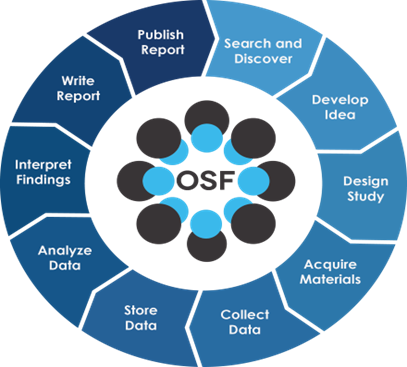
\includegraphics{img/osf-researchcycle.png}}

}

\caption{\label{fig-osf-researchcycle}OSF Research Lifecycle}

\end{figure}%

O material utilizado nesse módulo do curso segue de perto a proposta de
Olson et al. (2022), um \href{https://osf.io/yaqe8/}{projeto oficial do
COS} que possui recursos, modelos e práticas para ajudar os
pesquisadores a iniciar sua jornada \textbf{OSF}. Claro que ele foi
adaptado para nossos fins, principalmente, em decorrência do tempo
destinado ao módulo.

\begin{tcolorbox}[enhanced jigsaw, opacitybacktitle=0.6, titlerule=0mm, left=2mm, toptitle=1mm, opacityback=0, arc=.35mm, colback=white, rightrule=.15mm, breakable, leftrule=.75mm, bottomrule=.15mm, colbacktitle=quarto-callout-tip-color!10!white, colframe=quarto-callout-tip-color-frame, coltitle=black, bottomtitle=1mm, toprule=.15mm, title=\textcolor{quarto-callout-tip-color}{\faLightbulb}\hspace{0.5em}{\emph{Bifurcando ou duplicando um projeto}}]

Você sabia que é possível executar um ``\emph{forking}'' (criar uma
cópia do projeto existente) ou ``\emph{duplicate as template}''
(duplicar apenas a estrutura do projeto e seus componentes) de um
projeto público no OSF?\vspace{0.5em}

Você que se interessa em iniciar seu próprio projeto OSF com um modelo,
pode criar sua própria duplicata do projeto Olson et al. (2022) para
começar!\vspace{0.5em}

Neste \href{https://osf.io/yaqe8/}{projeto}, existem templates e
recursos básicos para diversos casos de uso encontrados no OSF;
coordenação de equipes de pesquisa, planejamento de gerenciamento de
dados, documentos reprodutíveis e até mesmo gerenciamento de cursos.

\end{tcolorbox}

Para os alunos que desejam uma leitura sobre o \textbf{OSF} na prática,
indicamos os artigos de Sullivan et al. (2019) e Soderberg (2018).
Apesar de o leitor poder encontrar \emph{prints} das telas da plataforma
desatualizadas, esses dois artigos podem ser um bom começo para entender
a lógica da plataforma. E \emph{off course}, recomendamos fortemente
você dar uma olhada no
\href{https://help.osf.io/article/342-getting-started-on-the-osf}{suporte
do \textbf{OSF}}, onde podemos encontrar vídeos introdutórios
excelentes.

Esse curso poderia ter sido concebido e gerenciado dentro do
\textbf{OSF}, no entanto, devido a proposta de apresentarmos também o
\href{https://phdpablo.github.io/curso-open-science/05-git.html}{Git/Github}
e sua integração com documentos reprodutíveis no
\href{https://phdpablo.github.io/curso-open-science/06-quarto.html}{RStudio/Quarto},
optamos por priorizar o repositório do Github. Por isso, que também
nesse módulo passamos pelo
\href{https://phdpablo.github.io/curso-open-science/00-prework.html\#sec-zenodoprework}{Zenodo},
que integra com o Github e tem a capacidade de gerar DOIs para as
versões dos repositórios.

\begin{tcolorbox}[enhanced jigsaw, opacitybacktitle=0.6, titlerule=0mm, left=2mm, toptitle=1mm, opacityback=0, arc=.35mm, colback=white, rightrule=.15mm, breakable, leftrule=.75mm, bottomrule=.15mm, colbacktitle=quarto-callout-note-color!10!white, colframe=quarto-callout-note-color-frame, coltitle=black, bottomtitle=1mm, toprule=.15mm, title=\textcolor{quarto-callout-note-color}{\faInfo}\hspace{0.5em}{\emph{Open and Reproducible Research on Open Science Framework}
(Tip~\ref{tip-prompt})}]

O artigo (Sullivan et al., 2019) apresenta um protocolo para a
implementação de práticas de Ciência Aberta (CA), com foco no uso do
Open Science Framework (OSF). As principais ideias do texto são as
seguintes:\vspace{0.5em}

\begin{itemize}
\item
  A CA é um movimento que promove a transparência, a reprodutibilidade e
  a acessibilidade dos resultados de pesquisa;
\item
  As práticas de CA podem contribuir para a melhoria da qualidade da
  pesquisa científica, tornando-a mais confiável e robusta;
\item
  O OSF é uma plataforma gratuita e de código aberto que pode ser usada
  para implementar práticas de CA;\vspace{0.5em}
\end{itemize}

O protocolo apresentado no texto fornece instruções passo a passo para
as seguintes práticas de CA:\vspace{0.5em}

\begin{itemize}
\item
  \textbf{Planejamento de gerenciamento de dados}: O planejamento de
  gerenciamento de dados é essencial para garantir que os dados de
  pesquisa sejam armazenados, organizados e gerenciados de forma
  eficiente e eficaz. O OSF fornece ferramentas para ajudar os
  pesquisadores a planejar e implementar seus planos de gerenciamento de
  dados.
\item
  \textbf{Pré-registro de estudos}: O pré-registro de estudos é uma
  prática que consiste em publicar um plano de pesquisa antes de iniciar
  o estudo. Isso ajuda a garantir que o estudo seja realizado de forma
  objetiva e transparente. O OSF fornece um recurso para pré-registrar
  estudos.
\item
  \textbf{Controle de versão}: O controle de versão é uma prática que
  consiste em rastrear as alterações feitas em arquivos de texto. Isso
  ajuda a garantir que os resultados de pesquisa sejam reprodutíveis e
  que as alterações feitas nos dados sejam rastreáveis. O OSF fornece
  ferramentas para gerenciar o controle de versão de arquivos de
  pesquisa.
\item
  \textbf{Compartilhamento de dados e materias}: O compartilhamento de
  dados e materiais de pesquisa é uma prática importante para aumentar a
  transparência e a reprodutibilidade da pesquisa. O OSF fornece um
  repositório para compartilhar dados e materiais de pesquisa.
\item
  \textbf{Publicação de pré-impressões}: As pré-impressões são versões
  preliminares de artigos científicos que são publicadas online antes de
  serem revisados por pares. As pré-impressões podem ajudar a acelerar a
  divulgação da pesquisa e a promover o debate científico. O OSF fornece
  um repositório para publicar pré-impressões.\vspace{0.5em}
\end{itemize}

O artigo fornece informações valiosas para os pesquisadores que desejam
implementar práticas de CA. O protocolo apresentado pode ser usado como
um guia para implementar essas práticas de forma eficaz.

\end{tcolorbox}

\bookmarksetup{startatroot}

\chapter{Gerenciamento de Referências e Bibliotecas}\label{sec-zotero}

Existem mais de 30 diferentes\footnote{\href{https://en.wikipedia.org/wiki/Comparison_of_reference_management_software}{Esta
  lista} no Wikipedia, que é atualizada constantemente, faz uma
  comparação entre eles.} gerenciadores de referências (Proske et al.,
2023). Entre eles podemos indicar o
\href{https://www.citavi.com/en}{Citavi} e o
\href{https://refworks.proquest.com/learn-more/}{RefWorks}. No entanto,
os mais populares são o \href{https://endnote.com/}{EndNote},
\href{https://www.mendeley.com/reference-management/reference-manager/}{Mendeley}
e \href{https://www.zotero.org/}{Zotero}. O primeiro é proprietário e
descartamos enquanto opção para nosso workflow de Open Science. Os dois
últimos são excelentes opções, no entanto, o Zotero se destaca por ser
código aberto (totalmente gratuíto), enquanto o Mendeley, embora
gratuito, é propriedade da Elsevier, uma editora comercial. Isso
significa que o Zotero não tem restrições de uso e não exige pagamento
por recursos adicionais, exceto por maior armazenamento na nuvem, que
inclusive, é um destaque do Mendeley (2Gb \emph{vs} 300Mb).

Além disso, o Zotero tem uma comunidade ativa e fóruns de suporte, o que
pode ser útil para solucionar problemas e compartilhar conhecimento com
outros usuários. Portanto, como aqui valorizamos a liberdade de código
aberto e uma comunidade engajada, o Zotero é nossa escolha.

Essa característica faz com que o Zotero se destaca em relação ao
Mendeley, especialmente no que diz respeito ao \textbf{Ecossitema de
Plugins}. O Zotero possui uma comunidade ativa de desenvolvedores e
pesquisadores que criam e compartilham plugins. Esses plugins estendem
as funcionalidades do Zotero, permitindo personalizações específicas e
integrações com outras ferramentas (Behera \& Jain, 2023). O plugin
\href{https://retorque.re/zotero-better-bibtex/}{Better BibTeX}, por
exemplo, oferece recursos avançados de exportação e formatação de
bibliografias, tornando-o uma escolha popular para usuários que
trabalham com LaTeX, Markdown, HTML, e outras linguagens de marcação.
Outro exemplo é o \href{https://zotfile.com/}{ZotFile}, que permite
gerenciar anexos de PDFs, renomeando arquivos automaticamente e
organizando-os em pastas específicas (Behera \& Jain, 2023). Assim,
poderás estender o armazenamento do Zotero de 300Mb para o limite de seu
serviço de armazenamento na nuvem (Google Drive, OneDrive, Dropbox,
etc.)\footnote{Outro importante plugin é a integração com o
  \href{https://github.com/ethanwillis/zotero-scihub}{SciHub} (Behera \&
  Jain, 2023). Coloquei essa informação em nota, pois ele é questionável
  do ponto de vista ético, apesar de extensivamente utilizado no Brasil
  por estudantes de pós-graduação stricto sensu de diferentes áreas
  (Oddone \& Souza, 2024). Ou se enxergarmos o problema sob outro ponto
  de vista, a ampla adoção do SciHub no Brasil e em todo o mundo reflete
  a resposta dos cientistas ao desgastado sistema de comunicação
  científica mantido pelas editoras internacionais.~Além disso, reforça
  a relevância dos princípios da Ciência Aberta (Oddone \& Souza, 2024).}.

Nesse sentido, uma recomendação importante é não deixar de dar uma
olhada no \href{https://www.zotero.org/support/plugins}{página de
plugins} do Zotero no site oficial e uma
\href{https://github.com/search?q=zotero&type=repositories}{busca por
Zotero} no Github. Com certeza você vai encontrar uma solução (plugin)
interessante para potencializar as funcionalidades do Zotero. Algumas
delas veremos ao longo do curso.

A mensagem principal que pretendemos passar no curso sobre esse tópico é
para você conceber os gerenciadores de referências e bibliotecas no
contexto do processo de escrita, e não apenas como facilitadores
operacionais (``\emph{time saver}'') de citações e bibliografias.
Somente usuários avançados podem aproveitar o suporte que a maioria dos
sistemas de gerenciamento de referências oferece para o processo de
escrita (Proske et al., 2023).

Atualmente, gerenciadores de referências mais populares oferecem
funcionalidades básicas, que incluem:

\begin{itemize}
\item
  Recursos para coletar referências com textos completos e organizá-las
  em pastas e/ou (sub)coleções;
\item
  Marcar entradas de referência, fazer anotações e destacar o texto
  completo por meio de visualizadores de PDF integrados;
\item
  Citar referências em diferentes estilos de citação por meio de
  complementos para software de processamento de texto ou criando e
  atualizando automaticamente arquivos BIB para outras linguagens de
  marcação;
\item
  Sincronizar referências entre o aplicativo de desktop e a versão
  móvel, bem como entre diferentes computadores; e
\item
  Compartilhar referências com colegas (Proske et al., 2023)
\end{itemize}

Esse conteúdo é abordado em detalhes no trabalho de Thomas (2023), e
veremos algumas dessas funcionalidades básica na aula, no entanto,
daremos ênfase no Ecossitema de Plugins do Zotero.

Para um curso mais aprofundado sobre o Zotero, recomendamos a playlist
de vídeos
\href{https://youtube.com/playlist?list=PLEbpo1iiweYXhQs1-yKJhTLPio1PlBD0i&si=bI3_sDEQe58XOCTf}{Zotero
do Zero} da Biblioteca Ciências da Saúde UFES. Neles, você aprenderá
praticamente tudo o que precisa saber para utilizar o Zotero de forma
nativa, com muitas dicas ocultas e truques, e ainda, como instalar e
configurar alguns plugins.

\bookmarksetup{startatroot}

\chapter{Gestão de Projetos}\label{sec-project}

Essa seção é o elo entre as seções anteriores e as próximas. Aqui, você
vai receber algumas dicas de como organizar seus dados, pasta e scripts
em um projeto de pesquisa. Talvez você se pergunte: porque eu preciso
aprender a organizar meus arquivos e pasta? Já faço isso, do meu jeito,
há anos, e nunca tive problemas em entender o que eu faço! A resposta é
simples: não trata somente de você entender e achar que o produto final
da sua pesquisa (o artigo) seja suficiente. No contexto da Ciência
Aberta (CA) a ideia é que deixe transparente o processo de análise,
materiais e métodos, e que outros pesquisadores possam reproduzir seus
resultados. Nesse sentido, deve haver uma padronização mínima de
organização de arquivos, pastas e scripts para que outros pesquisadores
possam entender e reproduzir seus resultados. Lembre-se que agora você
pode compartilhar uma pasta compilada da sua pesquisa, via Google Drive
ou OneDrive, no seu projeto do \href{https://osf.io/}{Open Science
Framework}.

Nesse sentido, a intenção é que adotemos certa padronização na
organização de arquivos, pastas e scripts, seguindo algumas sugestões de
boas práticas para que o processo da nossa pesquisa fique inteligível
para qualquer um. Para você ver tanto que a ``coisa'' é séria, existe
até protocolo de padronização de organização de arquivos e pastas, como
o \href{https://www.projecttier.org/}{Project TIER}, focado para
pesquisas em ciências sociais. No caso de scripts, talvez o estilo de
escrita e organização mais conhecido para o ambiente R seja o
\href{https://style.tidyverse.org/}{Tidyverse Style Guide}. O livro de
Zandonella Callegher \& Massidda (2022) apresenta uma excelente
discussão desses tópicos nos capítulos 3, 4 e 5\footnote{Na verdade, se
  tivéssemos que indicar um único livro de leitura para abordar os temas
  do curso, esse livro seria o recomendado. Apesar de não contextualizar
  a CA como fizemos no começo, nem apresentar o Zotero e outras
  ferramentas de IA dentro desse contexto, talvez seja o compêndio que
  mais se assemelha à proposta de nosso curso.}.

No entanto, pelo menos nesse primeiro momento, resolvemos discutir um
conjunto de boas práticas computacionais que todo pesquisador deve
adotar, independentemente do seu nível atual de habilidade
computacional, apresentadas por Wilson et al. (2017). Essas práticas
abrangem gerenciamento de dados, programação, colaboração com colegas,
organização de projetos, acompanhamento de trabalhos e redação de
manuscritos. Especificamente, na aula dessa seção detalhamos o ``Box 1.
Summary of practices'' do artigo (Wilson et al., 2017), que pontua 38
tópicos. Quais sejam:

\section{Gerenciamento de Dados}\label{gerenciamento-de-dados}

\begin{enumerate}
\def\labelenumi{\arabic{enumi}.}
\tightlist
\item
  \textbf{Proteção dos Dados Brutos}: Dados originais não devem ser
  sobrescritos. Usar permissões de somente leitura e garantir múltiplos
  backups em locais diferentes, como Google Drive e Dropbox, para evitar
  perda de dados.
\item
  \textbf{Conversão de Dados}: Transformar dados para formatos como CSV
  ou JSON sem alterar seu conteúdo facilita a análise e a visualização.
\item
  \textbf{Estruturação de Dados}: Cada coluna deve representar uma
  variável e cada linha, uma observação. Isso facilita a aplicação de
  técnicas de análise.
\item
  \textbf{Automatização e Documentação}: Utilizar scripts em R ou Python
  para todas as etapas do processamento de dados e manter um log
  detalhado das operações.
\item
  \textbf{Acessibilidade e Citação}: Tornar os dados acessíveis a outros
  pesquisadores e garantir a citação adequada ao compartilhar dados em
  repositórios como OSF ou Zenodo.
\end{enumerate}

\section{Programação}\label{programauxe7uxe3o}

\begin{enumerate}
\def\labelenumi{\arabic{enumi}.}
\tightlist
\item
  \textbf{Documentação}: Documentar o propósito e o uso dos programas
  ajuda na compreensão e manutenção futura.
\item
  \textbf{Modularização}: Dividir o código em funções separadas para
  carregamento de dados, limpeza e análise facilita a manutenção e
  reutilização.
\item
  \textbf{Redução de Redundância}: Usar bibliotecas existentes como
  Pandas em Python em vez de escrever código do zero.
\item
  \textbf{Teste de Código}: Escrever pequenos testes para verificar a
  funcionalidade correta do código.
\item
  \textbf{Publicação de Código}: Publicar código no Zenodo ou GitHub e
  gerar DOI para aumentar a visibilidade e reprodutibilidade.
\end{enumerate}

\section{Colaboração}\label{colaborauxe7uxe3o}

\begin{enumerate}
\def\labelenumi{\arabic{enumi}.}
\tightlist
\item
  \textbf{Gerenciamento de Projetos}: Utilizar ferramentas como Trello
  ou GitHub Issues para gerenciar tarefas e estabelecer canais de
  comunicação claros.
\item
  \textbf{Licenciamento e Citação}: Incluir arquivos de licença e
  citação nos repositórios de projetos.
\item
  \textbf{Documentação de Projeto}: Criar arquivos README.md e
  CITATION.md que descrevam o projeto, objetivos e como configurá-lo.
\item
  \textbf{Estrutura de Diretórios}: Organizar o projeto em diretórios
  nomeados de forma clara e manter todos os arquivos relacionados dentro
  deles.
\end{enumerate}

\section{Acompanhamento de
Mudanças}\label{acompanhamento-de-mudanuxe7as}

\begin{enumerate}
\def\labelenumi{\arabic{enumi}.}
\tightlist
\item
  \textbf{Versionamento com Git}: Fazer commits frequentes e de pequeno
  porte e sincronizar alterações com repositórios GitHub para manter um
  histórico detalhado das mudanças.
\item
  \textbf{Backup Automático}: Usar serviços de backup automático como
  Dropbox ou Google Drive para garantir a segurança dos dados.
\end{enumerate}

\section{Redação de Manuscritos}\label{redauxe7uxe3o-de-manuscritos}

\begin{enumerate}
\def\labelenumi{\arabic{enumi}.}
\tightlist
\item
  \textbf{Ferramentas de Versionamento}: Utilizar LaTeX, Markdown ou
  Quarto para redigir manuscritos, aproveitando a facilidade de
  versionamento e colaboração.
\item
  \textbf{Publicação e Compartilhamento}: Integrar práticas de ciência
  aberta no fluxo de trabalho, como publicar pré-prints e pré-registrar
  estudos.
\end{enumerate}

Em resumo, o artigo (Wilson et al., 2017) propõe que pesquisadores de
todas as áreas devem adotar práticas computacionais sólidas para
garantir a integridade, reprodutibilidade e transparência de suas
pesquisas.

E por fim, também sugerimos que os pesquisadores se engajem em
comunidades de práticas para compartilhar conhecimento e colaborar com
outros pesquisadores. Bora começar?

\section{Implementação de Ciência
Aberta}\label{implementauxe7uxe3o-de-ciuxeancia-aberta}

\begin{enumerate}
\def\labelenumi{\arabic{enumi}.}
\tightlist
\item
  \textbf{Começar Pequeno}: Iniciar com pequenas práticas de ciência
  aberta, como usar software de código aberto e publicar pré-prints.
\item
  \textbf{Conhecer Políticas}: Familiarizar-se com políticas de ciência
  aberta e compartilhar casos de sucesso.
\item
  \textbf{Educação em Ciência Aberta}: Incorporar práticas de ciência
  aberta no conteúdo dos cursos e adotar recursos educacionais abertos.
\item
  \textbf{Colaboração e Redes}: Desenvolver redes colaborativas e
  utilizar ferramentas abertas para repositórios e versionamento de
  dados.
\item
  \textbf{Mudança na Avaliação Acadêmica}: Promover alternativas à
  medição tradicional de desempenho acadêmico e reconhecer uma variedade
  de resultados de pesquisa.
\end{enumerate}

\section{Cenas dos próximos
capítulos}\label{cenas-dos-pruxf3ximos-capuxedtulos}

\url{https://www.youtube.com/watch?v=s3JldKoA0zw}

\begin{tcolorbox}[enhanced jigsaw, opacitybacktitle=0.6, titlerule=0mm, left=2mm, toptitle=1mm, opacityback=0, arc=.35mm, colback=white, rightrule=.15mm, breakable, leftrule=.75mm, bottomrule=.15mm, colbacktitle=quarto-callout-warning-color!10!white, colframe=quarto-callout-warning-color-frame, coltitle=black, bottomtitle=1mm, toprule=.15mm, title=\textcolor{quarto-callout-warning-color}{\faExclamationTriangle}\hspace{0.5em}{Você não vai querer cometer esses erros\ldots{}\footnote{Pedimos para o
  ChatGPT4o resumir as duas matérias e me nos dar resposta em português.
  Como sempre, revisamos o conteúdo para saber se batia com o que eu
  lemos.}}]

\href{https://www.bbc.com/news/magazine-22223190}{\textbf{Caso 1:
Reinhart, Rogoff\ldots{} e Herndon: O aluno que pegou os
professores}}\vspace{1em}

Economistas ficaram surpresos ao descobrir que um famoso artigo
acadêmico, frequentemente usado para justificar cortes de austeridade,
continha erros significativos. Esses erros, cometidos por dois renomados
professores de Harvard, foram identificados por um estudante durante a
realização de um trabalho acadêmico.\vspace{0.5em}

Em 4 de janeiro de 2010, no Marriott Hotel em Atlanta, durante a reunião
anual da American Economic Association, os professores Carmen Reinhart e
Ken Rogoff apresentaram um artigo chamado ``Growth in a Time of Debt''.
Eles afirmavam que o crescimento econômico desacelera drasticamente
quando a dívida de um país ultrapassa 90\% do Produto Interno Bruto
(PIB).\vspace{0.5em}

O artigo ganhou notoriedade rapidamente, sendo citado por formuladores
de políticas como o comissário da UE Olli Rehn e o político republicano
dos EUA Paul Ryan, que usaram o limite de 90\% de dívida-PIB para apoiar
estratégias de austeridade.\vspace{0.5em}

Thomas Herndon, um estudante da Universidade de Massachusetts Amherst,
escolheu este artigo para uma tarefa de replicação de resultados. No
entanto, Herndon não conseguiu replicar os resultados dos professores de
Harvard, o que inicialmente o fez pensar que havia cometido um erro.
Após várias verificações e com a ajuda de seus professores, Herndon
entrou em contato com Reinhart e Rogoff, que forneceram a planilha usada
na pesquisa original.\vspace{0.5em}

Ao analisar a planilha, Herndon descobriu um erro básico: os professores
de Harvard haviam incluído apenas 15 dos 20 países analisados em um
cálculo crucial. Além disso, havia outras questões metodológicas, como a
forma de mediação dos dados, que distorciam os resultados.\vspace{0.5em}

Esses achados foram publicados em 15 de abril, revelando que, embora
altos níveis de dívida ainda estejam correlacionados com menor
crescimento, a relação é muito mais suave e há muitas exceções à regra.
Reinhart e Rogoff reconheceram o erro, mas defenderam que ele não
afetava significativamente a mensagem central do artigo.\vspace{0.5em}

Essa descoberta trouxe à tona a importância de verificar e replicar
resultados de pesquisas, especialmente aquelas que influenciam políticas
públicas. Embora o debate sobre a austeridade continue, o trabalho de
Herndon destacou a necessidade de rigor acadêmico e a revisão crítica
dos estudos usados para fundamentar decisões econômicas.\vspace{0.5em}

\href{https://www.theverge.com/2020/8/6/21355674/human-genes-rename-microsoft-excel-misreading-dates}{\textbf{Caso
2: Cientistas renomeiam genes humanos para impedir que o Microsoft Excel
os interprete erroneamente como datas}}\vspace{1em}

Nos últimos anos, 27 genes humanos foram renomeados devido a um problema
comum com o Microsoft Excel, que interpretava incorretamente os símbolos
alfanuméricos dos genes como datas. Esse problema surgiu porque o Excel,
uma ferramenta amplamente utilizada por cientistas para gerenciar dados,
converte automaticamente certos símbolos de genes, como ``MARCH1''
(abreviação de ``Membrane Associated Ring-CH-Type Finger 1''), em datas,
como ``1-Mar''.\vspace{0.5em}

Estudos mostraram que cerca de um quinto dos dados genéticos em artigos
publicados foi afetado por erros do Excel. Esse problema é tão difundido
que até mesmo trabalhos revisados por pares foram impactados. Não há uma
solução fácil, já que o Excel não permite desativar essa formatação
automática. Para contornar isso, os cientistas precisam alterar
manualmente o tipo de dado para cada coluna ou corrigir os dados sempre
que exportam e importam arquivos.\vspace{0.5em}

Para resolver esse problema, o Comitê de Nomenclatura de Genes da HUGO
(HGNC) publicou novas diretrizes para a nomeação de genes, levando em
consideração o comportamento do Excel. Por exemplo, ``MARCH1'' foi
alterado para ``MARCHF1'' e ``SEPT1'' para ``SEPTIN1''. Essas mudanças
foram implementadas após consultar a comunidade científica para evitar
confusões futuras.\vspace{0.5em}

Historicamente, a nomeação de genes permitia certa criatividade,
resultando em nomes curiosos como ``sonic hedgehog'' e ``Indy''. No
entanto, as diretrizes atuais priorizam a clareza e a praticidade,
exigindo nomes únicos e específicos, que evitem confusões e termos
ofensivos.\vspace{0.5em}

Embora houvesse algum debate sobre por que os cientistas deveriam
ajustar os nomes dos genes em vez de o Excel mudar sua funcionalidade, a
decisão foi baseada na praticidade. A mudança no Excel beneficiaria
apenas um pequeno grupo de usuários, enquanto a renomeação dos genes
oferece uma solução imediata e duradoura.\vspace{0.5em}

Essa mudança foi bem recebida pela comunidade científica, que expressou
entusiasmo nas redes sociais pela resolução de um problema que afetava
significativamente o trabalho de pesquisa.\vspace{0.5em}

Essa decisão ilustra como a ciência pode se adaptar para superar
desafios práticos, garantindo que a pesquisa continue de maneira
eficiente e precisa.\vspace{0.5em}

\end{tcolorbox}

\bookmarksetup{startatroot}

\chapter{Controle de versão}\label{sec-git}

Você\footnote{A \href{https://git-scm.com/book/en/v2}{literatura sobre
  controle de versão}, especialmente Git e Github, é ``farta''. Tanto em
  inglês como em português. Uma pesquisa simples vai achar muitas
  referências a blogs e textos de profissionais especializados,
  inclusive, \href{https://happygitwithr.com/}{para os nossos fins}. No
  Youtube existem muitos vídeos sobre o tema. Seja o que escrevessemos
  por aqui, seria de pouca contribuição. Dessa forma, buscamos
  contextualizar o versionamento de arquivos num empreendimento de
  pesquisa de nosso dia a dia: um pesquisador com viés quantitativo,
  envolvido em pesquisas sem pouca colaboração, mas que achou no
  controle de versão uma solução impar para diversas demandas
  preconizadas pela Ciência Aberta.} em algum grau utiliza um sistema
para versionar seu trabalho. Seja ele um simples \texttt{Ctrl\ +\ Z} ou
\texttt{Cmd\ +\ Z} para desfazer a última ação, ou sistemas mais
elaborados, como i) o controle de alterações do seu processador de texto
ou ii) o histórico de versões do seu aplicativo de armazenamento nas
nuvens (\texttt{OneDrive}, \texttt{Google\ Drive} ou \texttt{Dropbox}),
você já está familiarizado com a ideia de controle de versão. Qual
estudante ou pesquisador nunca se deparou com uma situação parecida da
Figura~\ref{fig-funny-git}?

\begin{figure}

\centering{

\href{https://phdcomics.com/comics/archive.php?comicid=1531}{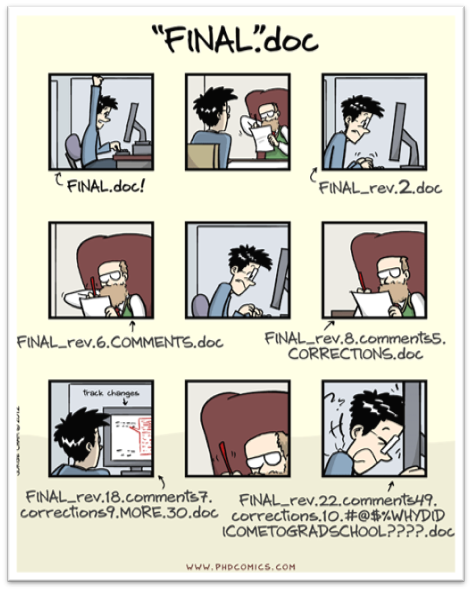
\includegraphics{img/funny-git.png}}

}

\caption{\label{fig-funny-git}Situação amadora de controle de versão}

\end{figure}%

No entanto, essas soluções são limitadas e não são adequadas para
gerenciar projetos de pesquisa complexos, ou mesmo simples, pois no
contexto da Ciência Aberta (CA), falham nos quesitos para
reprodutibilidade e transparência. Para isso, é necessário um sistema de
controle de versão (VCS) mais robusto, como o Git. O Git é um VCS
distribuído, ou seja, ele armazena o histórico de alterações em um
repositório local e remoto, permitindo que você controle as versões de
seus arquivos e compartilhe-os com outras pessoas. O Git é amplamente
utilizado em projetos de desenvolvimento de software, mas também é uma
ferramenta valiosa para pesquisadores que desejam gerenciar e
compartilhar seus ativos de pesquisa.

Os controles\footnote{Como ressaltamos na nota anterior\ldots{} nossa
  impressão era que não havia nada para dizer sobre o tema, haja vista a
  vasta literatura. Desse modo, resolvemos fazer um experimento e nessa
  nota documentamos para vocês. Dentro do enredo que adotamos para a
  aula e o roteiro dessa seção, conversamos com o ChatGPT 4o (em
  2024-06-19) e me apropriamos de alguns de seus argumentos para
  escrever o resto dessa seção. Claro, com muitos, mas muitos ajustes!
  Inclusive, a parte final dessa seção, onde conversamos sobre um
  hipotético workflow (Gitflow) para uma colaboração científica é de
  nossa propriedade. Seguem nossas prompts:

  \begin{itemize}
  \tightlist
  \item
    \emph{Sou pesquisador em ciências sociais aplicadas e estou
    escrevendo um artigo em que discuto o controle de versão, através do
    Git e Github, como um importante aliado das boas práticas da Ciência
    Aberta. Comecei contextualizando os controles de versionamento mais
    simples, tais como o controle de alterações de um processador de
    texto e histórico de versões de soluções de armazenamento nas
    nuvens. Me indique situações em que esses tipos de versionamentos
    não atendem um fluxo de trabalho de uma pesquisa empírica no
    contexto da ciência aberta.}
  \end{itemize}

  \textbf{Continuando a conversa\ldots{}}

  \begin{itemize}
  \tightlist
  \item
    \emph{No meu enredo argumento que o Git e Github são ``coisas''
    diferentes e o pesquisador, se quiser, desenvolve seu workflow
    apenas localmente com o Git. Compare o Git e Github em termos de
    soluções propostas para o versionamento para eu apresentar como
    exemplo de meus argumentos.}
  \end{itemize}

  \textbf{Continuando a conversa\ldots{}}

  \begin{itemize}
  \tightlist
  \item
    \emph{Certo, gostei da comparação, mas gostaria que desenvolvesse
    sua resposta na forma de um texto descritivo e não na forma de
    bullets points.}
  \end{itemize}

  \textbf{Continuando a conversa\ldots{}}

  \begin{itemize}
  \tightlist
  \item
    \emph{Certo, era exatamente isso que precisava para meus argumentos
    nesse ponto do artigo. No entanto, desejo finalizar com o seguinte
    enredo: o Git/Github são preparados para projetos muito complexos
    (cite cases para exemplificar esse argumento), mas suas
    funcionalidades também podem atender projetos de pesquisas mais
    simples que envolvam três pesquisadores ou um único pesquisador.
    Preciso de sua ajuda para desenvolver esses argumentos sem você
    repetir argumentos que já apresentou para mim nessa conversa.}
  \end{itemize}} de versionamento mais simples, como os oferecidos por
processadores de texto e soluções de armazenamento em nuvem, são
insuficientes para um workflow de pesquisa empírica no contexto da CA:

\begin{enumerate}
\def\labelenumi{\arabic{enumi}.}
\tightlist
\item
  \textbf{Colaboração Extensiva}:

  \begin{itemize}
  \tightlist
  \item
    Em projetos que envolvem múltiplos colaboradores, as ferramentas
    simples de versionamento podem dificultar o rastreamento e a fusão
    de contribuições de vários pesquisadores. O Git, por outro lado,
    oferece um sistema robusto de gerenciamento de branches e fusão de
    código, permitindo uma colaboração mais eficiente e organizada.
  \end{itemize}
\item
  \textbf{Rastreamento Detalhado de Mudanças}:

  \begin{itemize}
  \tightlist
  \item
    Processadores de texto e armazenamento em nuvem geralmente oferecem
    um histórico de versões limitado e pouco detalhado. Em contraste, o
    Git permite um rastreamento minucioso de cada alteração, incluindo o
    autor e o propósito de cada mudança, facilitando auditorias e
    revisões.
  \end{itemize}
\item
  \textbf{Gerenciamento de Código e Dados}:

  \begin{itemize}
  \tightlist
  \item
    Pesquisas empíricas frequentemente envolvem scripts de análise e
    grandes volumes de dados que necessitam de versionamento.
    Ferramentas simples de controle de versão não são otimizadas para
    esses tipos de arquivos, enquanto o Git é projetado para gerenciar
    código e dados de maneira eficiente, garantindo a integridade e
    reprodutibilidade das análises.
  \end{itemize}
\item
  \textbf{Automação e Integração Contínua}:

  \begin{itemize}
  \tightlist
  \item
    Em um ambiente de CA, é crucial automatizar testes e validações para
    garantir a qualidade e a reprodutibilidade dos resultados. Soluções
    como GitHub Actions permitem a implementação de pipelines de
    integração contínua (CI), automatizando testes e outras tarefas,
    algo que não é possível com controles de versão simples.
  \end{itemize}
\item
  \textbf{Documentação e Transparência}:

  \begin{itemize}
  \tightlist
  \item
    O Git e o GitHub incentivam a documentação detalhada através de
    commit messages e issues, promovendo a transparência e o
    entendimento do progresso e das decisões do projeto. Ferramentas
    simples de versionamento não oferecem mecanismos equivalentes para
    documentar o processo de desenvolvimento de forma estruturada.
  \end{itemize}
\item
  \textbf{Resolução de Conflitos}:

  \begin{itemize}
  \tightlist
  \item
    Em projetos complexos, conflitos de versão são inevitáveis. Sistemas
    simples de versionamento podem não oferecer ferramentas adequadas
    para resolver esses conflitos de maneira eficiente. O Git
    proporciona ferramentas avançadas de merge e resolução de conflitos,
    minimizando o risco de perda de dados ou inconsistências.
  \end{itemize}
\item
  \textbf{Histórico Completo e Analítico}:

  \begin{itemize}
  \tightlist
  \item
    Ferramentas simples geralmente mantêm um histórico limitado, focado
    em versões específicas de documentos. O Git mantém um histórico
    completo e analítico de todas as mudanças, permitindo análises
    detalhadas do desenvolvimento do projeto ao longo do tempo.
  \end{itemize}
\end{enumerate}

Git e GitHub são ferramentas intimamente relacionadas, mas oferecem
soluções distintas para o versionamento, atendendo a diferentes
necessidades dos pesquisadores.

Git é um sistema de controle de versão distribuído que permite aos
usuários rastrear alterações em arquivos e coordenar o trabalho em
projetos colaborativos. Uma das principais vantagens do Git é a
capacidade de operar de forma totalmente local. Isso significa que os
pesquisadores podem manter um histórico completo de alterações em seus
arquivos sem a necessidade de conexão com a internet ou de um servidor
externo. Essa funcionalidade é particularmente útil para aqueles que
preferem manter seus dados em um ambiente controlado e privado.

Além disso, Git oferece funcionalidades avançadas de branching e
merging. Isso permite que diferentes linhas de trabalho sejam
desenvolvidas simultaneamente e depois combinadas de maneira controlada.
Essa flexibilidade é essencial para experimentações e desenvolvimentos
paralelos, comuns em projetos de pesquisa. O rastreamento detalhado é
outra característica fundamental do Git. Cada commit no sistema é
identificado de forma única e inclui metadados sobre quem fez a
alteração e uma mensagem descritiva, permitindo um histórico minucioso
das mudanças. Caso seja necessário, Git permite reverter para estados
anteriores do projeto, recuperando versões passadas sem perder o
histórico de alterações. Como um sistema distribuído, Git realiza
operações de controle de versão localmente, o que resulta em um
desempenho rápido e eficiente, sem depender da latência de rede.

Por outro lado, GitHub é uma plataforma baseada na web que utiliza o Git
como backend e adiciona funcionalidades colaborativas e de gerenciamento
de projetos. Uma das maiores vantagens do GitHub é a hospedagem de
repositórios Git, permitindo que os pesquisadores façam backup de seus
projetos na nuvem e colaborem com outros usuários de qualquer lugar do
mundo. Isso facilita a colaboração extensiva, um aspecto crucial no
contexto da CA.

GitHub também fornece ferramentas como pull requests e reviews de
código, que simplificam a colaboração entre diferentes pesquisadores.
Essas ferramentas permitem que propostas de mudanças sejam discutidas,
revisadas e integradas de forma estruturada, promovendo um fluxo de
trabalho colaborativo e transparente. Além disso, GitHub Actions oferece
suporte à automação de testes, builds e outras tarefas, garantindo que
cada alteração seja verificada e validada automaticamente. Essa
funcionalidade é vital para assegurar a reprodutibilidade e a qualidade
do projeto, aspectos centrais da CA.

A plataforma GitHub também se destaca em termos de documentação e
comunicação. Issues, wikis e páginas de projetos proporcionam meios para
uma documentação detalhada, rastreamento de problemas e comunicação
eficiente entre os membros da equipe. O controle de acesso e permissões
é outro ponto forte do GitHub, permitindo que os gestores de projetos
configurem quem pode fazer alterações ou revisar o código, assegurando a
integridade do trabalho.

Além de todas essas funcionalidades, a hospedagem de projetos no GitHub
aumenta significativamente a visibilidade da pesquisa. Isso facilita a
disseminação de resultados e a colaboração com a comunidade científica
global, promovendo uma cultura de transparência e compartilhamento de
conhecimento.

Em resumo, enquanto o Git fornece uma solução robusta para controle de
versão local, ideal para quem necessita de um ambiente privado e
eficiente, o GitHub expande essas capacidades com ferramentas que
promovem a colaboração, automação, documentação e visibilidade pública.
No contexto da CA, o GitHub se alinha melhor com os princípios de
transparência, colaboração e reprodutibilidade, oferecendo um conjunto
de ferramentas que suportam e amplificam as boas práticas da pesquisa
científica.

Git e GitHub têm sido fundamentais em projetos de grande escala, como o
desenvolvimento do kernel do Linux e projetos de software de código
aberto como o TensorFlow, mantido pelo Google. Estes projetos envolvem
milhares de colaboradores ao redor do mundo, exigindo um sistema robusto
de controle de versão que possa lidar com uma vasta quantidade de
alterações simultâneas, fusões complexas e um alto nível de coordenação
e colaboração. A capacidade do Git de gerenciar branches de forma
eficiente e a integração contínua proporcionada pelo GitHub são
elementos cruciais para o sucesso desses projetos. A
Figura~\ref{fig-gitflow} ilustra um diagrama hipotético do fluxo de
trabalho em um ambiente de desenvolvimento de software típico, com
diversos ramos, e como a complexidade de gerenciamento de versões,
apesar de tratada pelo Git e GitHub, pode escalar.

\begin{figure}

\href{https://www.theserverside.com/blog/Coffee-Talk-Java-News-Stories-and-Opinions/Gitflow-release-branch-process-start-finish}{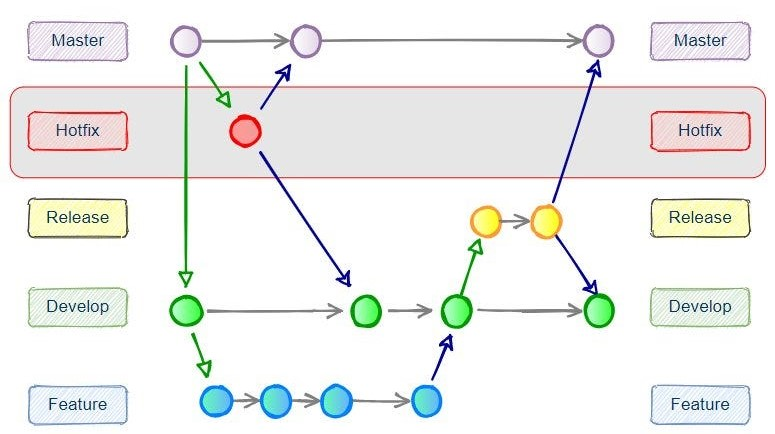
\includegraphics{img/gitflow.jpg}}

\caption{\label{fig-gitflow}Diagrama GitFlow hipotético num ambiente de
desenvolvimento de software típico}

\end{figure}%

No entanto, o Git/Github são igualmente valiosos para projetos de menor
escala. Em um projeto de pesquisa envolvendo três pesquisadores, Git e
GitHub facilitam a colaboração ao permitir que cada pesquisador trabalhe
em diferentes partes do projeto simultaneamente. Eles podem criar
branches individuais para testar novas hipóteses ou desenvolver partes
do projeto de forma independente. Quando uma nova contribuição está
pronta, ela pode ser integrada ao projeto principal através de um pull
request no GitHub, permitindo uma revisão por pares antes da fusão. Isso
não só mantém a qualidade do trabalho como também documenta o processo
de desenvolvimento de maneira transparente.

A Figura~\ref{fig-git3autores} ilustra um Gitflow hipotético para uma
colaboração científica envolvendo três autores. Note que cada autor tem
seu próprio branch de produção, que é integrado ao branch principal
através de pull requests, administrado pelo autor principal. Essa
estrutura permite que cada autor trabalhe de forma independente,
mantendo um histórico detalhado de suas contribuições e facilitando a
revisão e a fusão de alterações. Com apenas três branches, o
gerenciamento dessa hipotética pesquisa não seria tão complexo com o Git
e GitHub.

\begin{figure}

\href{https://doi.org/10.5281/zenodo.12165926}{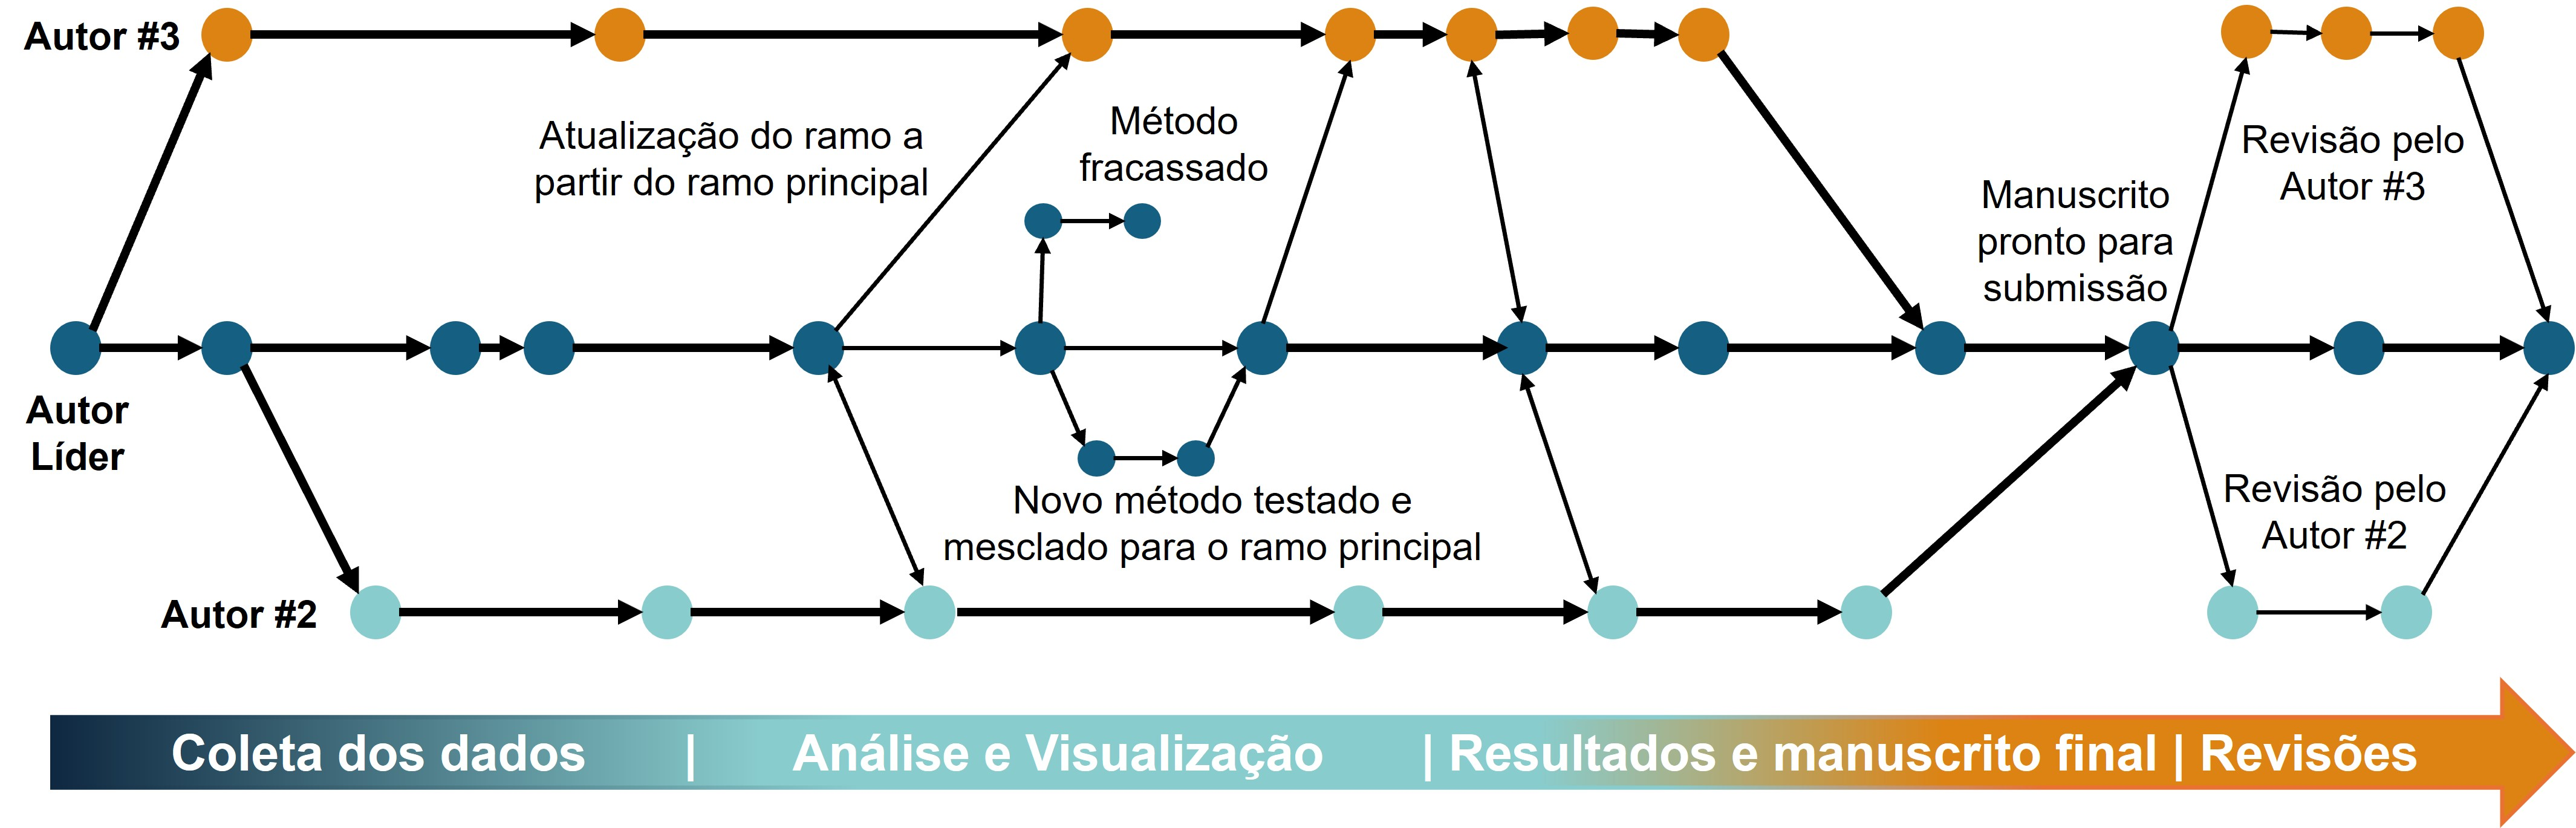
\includegraphics{img/git3autores.jpg}}

\caption{\label{fig-git3autores}Um fluxo de trabalho hipotético do Git
para uma colaboração científica envolvendo três autores. Cada círculo
representa um commit e as cores indicam commits específicos do autor.
Setas bidirecionais indicam uma sincronização (um push e pull na
terminologia Git). Setas unidirecionais indicam uma atualização de uma
ramificação para outra. As setas horizontais indicam o desenvolvimento
ao longo de um ramo específico . Ilustração disponível em:
\textless https://doi.org/10.5281/zenodo.12165926\textgreater.}

\end{figure}%

Para um único pesquisador, o Git oferece uma maneira eficaz de versionar
seu trabalho, mantendo um histórico detalhado de todas as alterações.
Isso pode ser especialmente útil para rastrear o progresso ao longo do
tempo, revertendo alterações se necessário e experimentando diferentes
abordagens sem o risco de perder trabalho anterior. Além disso, o GitHub
fornece um backup seguro na nuvem, garantindo que os dados estejam
protegidos contra perda.

A Figura~\ref{fig-gitautorbegin} ilustra um Gitflow hipotético para um
único pesquisador. Neste caso, o pesquisador mantém um branch principal
para o desenvolvimento do projeto e cria branches individuais para
experimentos ou novas ideias. Cada commit é documentado com uma mensagem
descritiva, permitindo que o pesquisador rastreie o progresso e o
propósito de cada alteração. Esse processo garante que o projeto seja
desenvolvido de forma estruturada e transparente, com um histórico
detalhado de todas as contribuições, que podem ser acompanhadas,
revisadas e auditadas por qualquer pessoa interessada, se o repositório
remoto for público.

\begin{figure}

\href{https://doi.org/10.5281/zenodo.12165926}{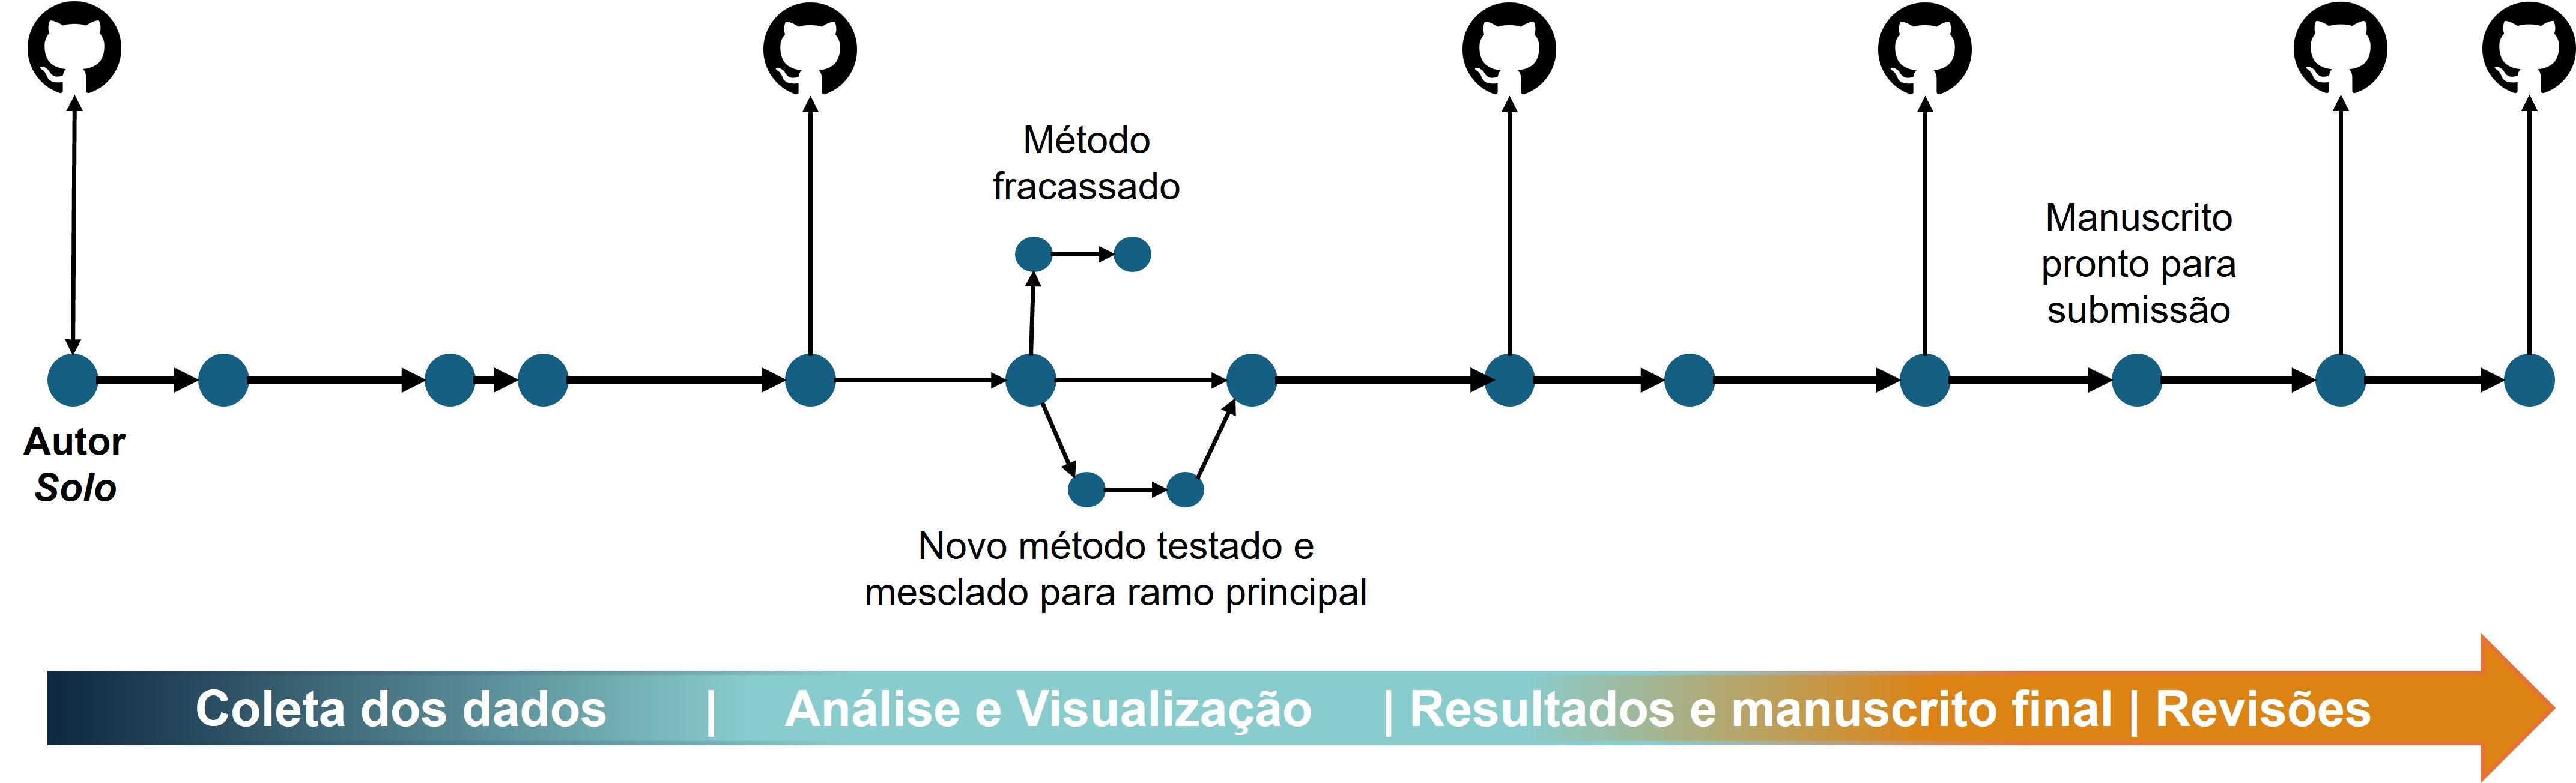
\includegraphics{img/gitautorbegin.jpg}}

\caption{\label{fig-gitautorbegin}Um fluxo de trabalho hipotético do Git
para a execução de uma pesquisa solo. Cada círculo representa um commit
específico do autor. Setas bidirecionais indicam uma sincronização (um
push ou pull na terminologia Git). Setas unidirecionais indicam uma
atualização de uma ramificação para outra. As setas horizontais indicam
o desenvolvimento ao longo de um ramo específico. Nesse fluxo de
trabalho o autor optou por sincronizar o repositório local com o
repositório remoto (Github) desde as etapas iniciais da pesquisa. Nessa
perspectiva o repositório remoto funciona como um armazenamento de
backup, e se público, para tornar a evolução do trabalho do pesquisador
disponível para quem deseja acompanhar. Ilustração disponível em:
\textless https://doi.org/10.5281/zenodo.12165926\textgreater{}}

\end{figure}%

Por outro lado, um pesquisador pode optar por tornar público seu
trabalho (dados, materiais e histórico de mudanças) somente quando for
submeter o artigo para publicação, como podemos ver na
Figura~\ref{fig-gitautorend}. Essa figura ilustra um workflow em que o
pesquisador desenvolveu seu trabalho localmente, fazendo uso do Git para
seu controle de versões, e apenas quando da necessidade de tornar
público, vinculou o repositório local com o repositório remoto.

\begin{figure}

\href{https://doi.org/10.5281/zenodo.12165926}{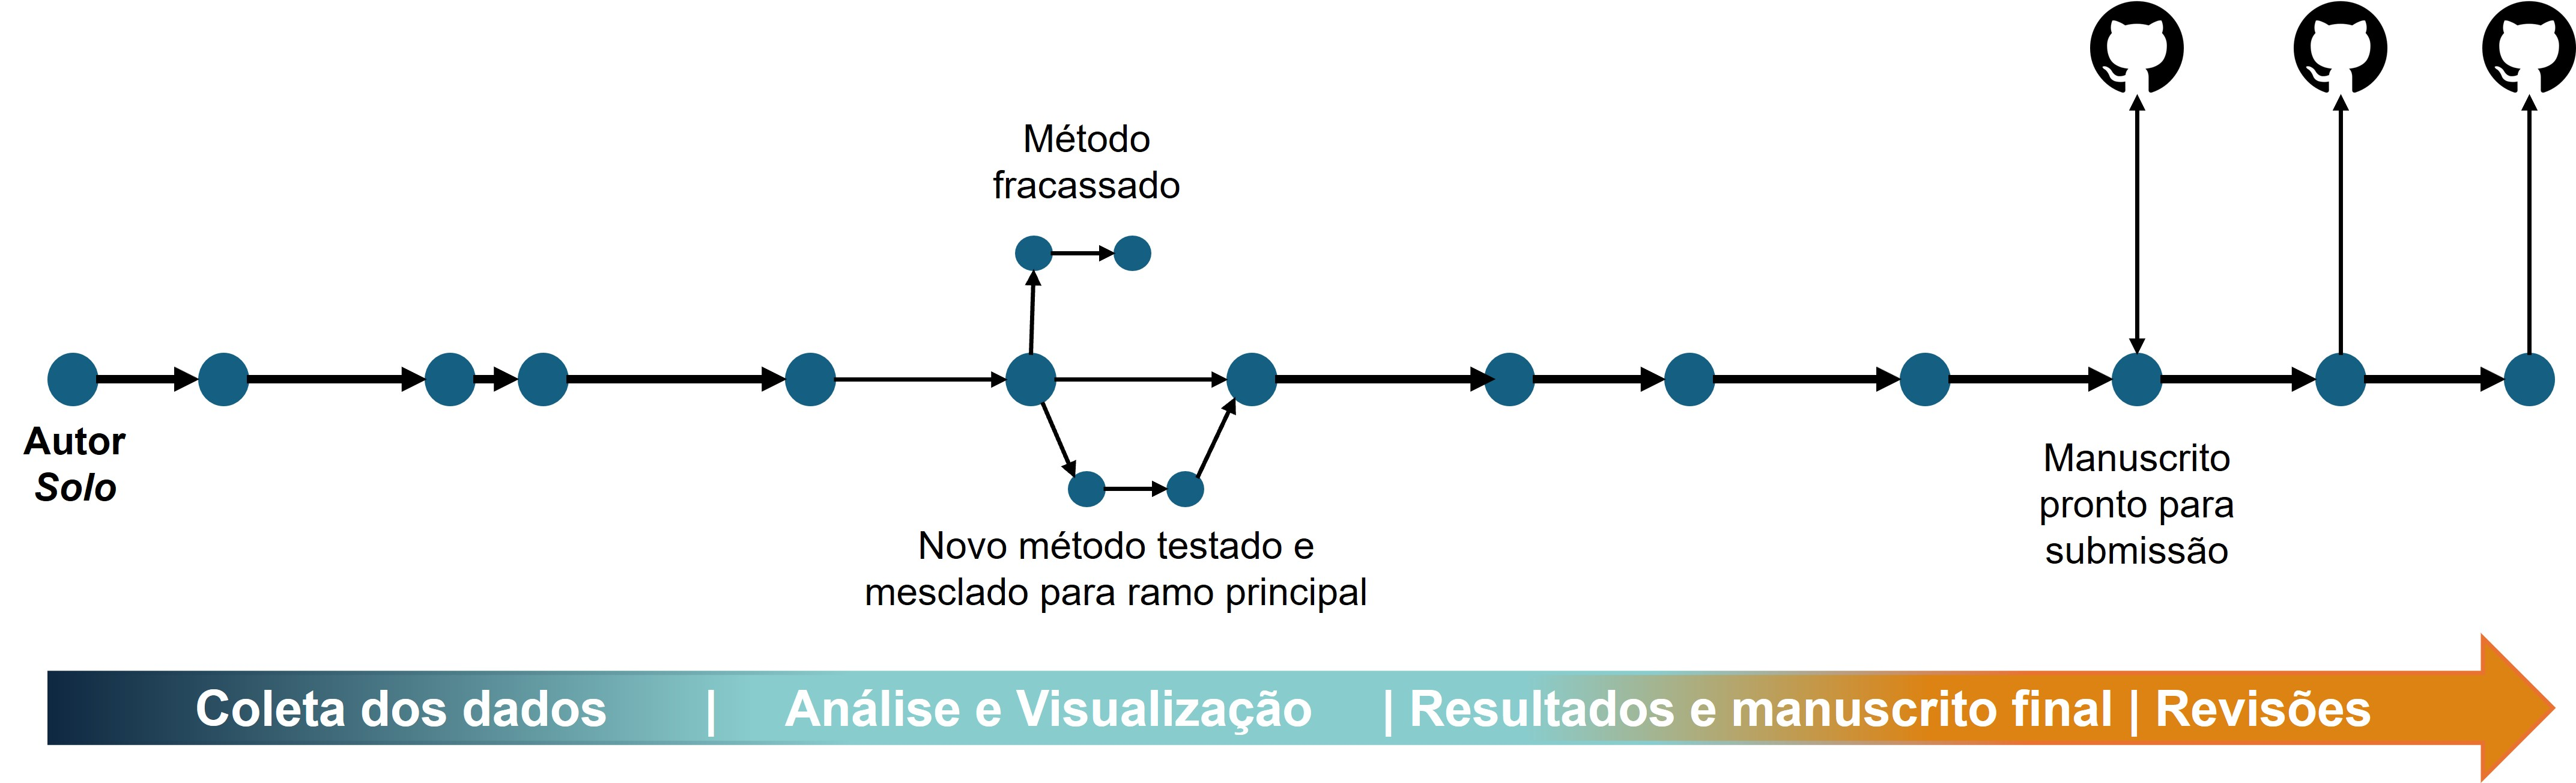
\includegraphics{img/gitautorend.jpg}}

\caption{\label{fig-gitautorend}Um fluxo de trabalho hipotético do Git
para a execução de uma pesquisa solo. Cada círculo representa um commit
específico do autor. Setas bidirecionais indicam uma sincronização (um
push ou pull na terminologia Git). Setas unidirecionais indicam uma
atualização de uma ramificação para outra. As setas horizontais indicam
o desenvolvimento ao longo de um ramo específico. Nesse fluxo de
trabalho o autor optou por sincronizar o repositório local com o
repositório remoto (Github) somente quando finalizou o artigo. Nessa
perspectiva o repositório remoto só faz sentido se para publicar os
dados, materiais da pesquisa e o histórico de mudanças, pois como
backup, o autor pode utilizar um serviço de armazenamento nas nuvens
(OneDrive, GoogleDrive, DropBox, etc.). Ilustração disponível em:
\textless https://doi.org/10.5281/zenodo.12165926\textgreater{}}

\end{figure}%

Embora sejam projetadas para lidar com projetos extremamente complexos,
as funcionalidades do Git/Github também se adaptam perfeitamente a
projetos de pesquisa mais simples, seja com número pequeno de
pesquisadores ou mesmo com um único pesquisador.

\begin{tcolorbox}[enhanced jigsaw, opacitybacktitle=0.6, titlerule=0mm, left=2mm, toptitle=1mm, opacityback=0, arc=.35mm, colback=white, rightrule=.15mm, breakable, leftrule=.75mm, bottomrule=.15mm, colbacktitle=quarto-callout-note-color!10!white, colframe=quarto-callout-note-color-frame, coltitle=black, bottomtitle=1mm, toprule=.15mm, title=\textcolor{quarto-callout-note-color}{\faInfo}\hspace{0.5em}{\emph{Curating Research Assets: A Tutorial on the Git Version Control
System} (Tip~\ref{tip-prompt})}]

Como uma tentativa de enfrentar os desafios da reprodutibilidade na
ciência empírica, um fator específico que se destaca é a forma como os
pesquisadores organizam, curam, compartilham e colaboram em seus ativos
de pesquisa (Vuorre \& Curley, 2018). Para mitigar essas dificuldades,
sistemas de controle de versão (VCS), como o Git, têm sido amplamente
adotados, uma vez que facilitam o acompanhamento das mudanças, versões e
colaboração em projetos científicos.\vspace{0.5em}

O Git, inicialmente desenvolvido para a escrita colaborativa de código,
agora é amplamente utilizado em diversas áreas além da ciência da
computação. Isso se deve à sua capacidade de tratar qualquer texto
digitado em um computador -- manuscritos, scripts de análise
estatística, código-fonte de experimentos computadorizados e até
arquivos de dados -- como código, gerenciando assim múltiplas versões e
autores sem introduzir erros (Vuorre \& Curley, 2018).\vspace{0.5em}

Ao trabalhar com Git, os usuários podem salvar versões intermediárias de
seus arquivos no disco rígido e, subsequentemente, no histórico do VCS.
Esse processo permite que todas as alterações sejam monitoradas e
revertidas quando necessário. A instalação do Git e sua integração com
ferramentas como o RStudio proporcionam uma interface gráfica amigável
para gerenciar repositórios locais e remotos, facilitando o controle de
versões e a colaboração (Vuorre \& Curley, 2018).\vspace{0.5em}

A introdução do Git desde o início de um projeto científico torna o
fluxo de trabalho mais eficiente e menos trabalhoso do que tentar
incorporar práticas de reprodutibilidade após a conclusão do projeto. A
organização clara de arquivos e pastas, seguindo diretrizes como as
recomendações do Project TIER, é uma etapa inicial crucial para garantir
a reprodutibilidade (Vuorre \& Curley, 2018).\vspace{0.5em}

O GitHub, uma plataforma online para hospedagem de repositórios Git,
permite a criação de repositórios centralizados que facilitam o trabalho
colaborativo. Os usuários podem clonar esses repositórios para suas
máquinas locais, fazer mudanças e enviar (push) essas alterações de
volta para o repositório central, assim como obter (pull) as alterações
feitas por outros colaboradores. Esse fluxo de trabalho centralizado
evita problemas de sobrescrita de arquivos e mantém um histórico
detalhado das contribuições de cada membro da equipe (Vuorre \& Curley,
2018).\vspace{0.5em}

No entanto, é importante notar que o Git não é a única solução para
colaboração e curadoria de materiais de pesquisa. Embora plataformas
como Google Docs e Dropbox ofereçam funcionalidades de colaboração em
tempo real e acesso ao histórico de arquivos, o Git proporciona
vantagens significativas para projetos mais complexos. Ele permite o
gerenciamento simultâneo de múltiplos componentes de um projeto, como
dados, scripts de análise e manuscritos, reduzindo a possibilidade de
erros associados ao uso de versões desatualizadas de arquivos (Vuorre \&
Curley, 2018).\vspace{0.5em}

Além disso, a utilização do Git com o RStudio é particularmente atrativa
para psicólogos, pois o ambiente integrado de desenvolvimento (IDE) do
RStudio, juntamente com os pacotes R Markdown (e Quarto) e knitr,
oferece uma solução completa para gestão de projetos, análise de dados e
preparação de manuscritos (Vuorre \& Curley, 2018). A integração com
serviços como Zenodo, que permite a atribuição de DOIs (identificadores
digitais) aos repositórios do GitHub, também facilita a citação dos
materiais de pesquisa (Vuorre \& Curley, 2018).\vspace{0.5em}

Em suma, a adoção de sistemas de controle de versão como o Git,
especialmente quando integrados a plataformas como o RStudio e o GitHub,
proporciona uma solução elegante para os desafios de curadoria,
compartilhamento e colaboração em ativos de pesquisa, contribuindo
significativamente para a melhoria da reprodutibilidade na ciência.

\end{tcolorbox}

\begin{tcolorbox}[enhanced jigsaw, opacitybacktitle=0.6, titlerule=0mm, left=2mm, toptitle=1mm, opacityback=0, arc=.35mm, colback=white, rightrule=.15mm, breakable, leftrule=.75mm, bottomrule=.15mm, colbacktitle=quarto-callout-note-color!10!white, colframe=quarto-callout-note-color-frame, coltitle=black, bottomtitle=1mm, toprule=.15mm, title=\textcolor{quarto-callout-note-color}{\faInfo}\hspace{0.5em}{\emph{Furthering Open Science in Behavior Analysis: An Introduction and
Tutorial for Using} \emph{GitHub in Research} (Tip~\ref{tip-prompt})}]

Este tutorial (Gilroy \& Kaplan, 2019) revisa as diretrizes de Práticas
Transparentes e Abertas fornecidas pela Open Science Foundation e
explora como os pesquisadores podem utilizar a transparência do GitHub
em suas pesquisas. Ele exemplifica como os pesquisadores podem usar o
GitHub para compartilhar código, dados e materiais de pesquisa,
permitindo a inspeção e replicação por parte de revisores e outros
pesquisadores através do \textbf{Github Desktop}.\vspace{0.5em}

As implicações do aumento da demanda por transparência e métodos
estatísticos modernos são discutidas, e plataformas como o GitHub são
revisadas como uma forma de apoiar a pesquisa
transparente.\vspace{0.5em}

A ``crise de reprodutibilidade'' é mencionada, referindo-se às
tentativas malsucedidas de replicar efeitos estatisticamente
significativos relatados em estudos psicológicos. As pressões para
publicar em revistas prestigiadas e obter financiamento são destacadas
como fatores que contribuem para a presença de práticas questionáveis de
pesquisa em várias disciplinas, incluindo psicologia.\vspace{0.5em}

A importância da transparência e da abertura é enfatizada como uma
maneira de enfrentar essas questões. As diretrizes TOP (Transparent and
Open Practices) são mencionadas, estabelecendo padrões para a
transparência em citações, dados, análises, materiais de pesquisa,
pré-registros e suporte para replicações. No entanto, é observado que
poucos estudos utilizam o pré-registro dos métodos e planos
analíticos.\vspace{0.5em}

O OSF e o GitHub são apresentados como plataformas que oferecem recursos
relacionados à pesquisa, como pré-registro e arquivamento público. O
GitHub é descrito como um serviço amplamente utilizado para arquivar e
gerenciar projetos de pesquisa. O controle de versão baseado em Git é
destacado como uma ferramenta de arquivamento robusta para pesquisa
analítica atual e futura. A importância de compartilhar o código-fonte,
dados e materiais do estudo é mencionada, permitindo a inspeção e
replicação por parte de revisores e outros pesquisadores. O foco do
tutorial é na execução do Github Desktop, uma interface gráfica para o
Git (Git Client), que facilita a colaboração e o controle de
versão.\vspace{0.5em}

A configuração adequada da máquina local é mencionada como necessária
para executar os programas estatísticos e scripts de análise. O processo
de bifurcação de um repositório no GitHub é explicado, assim como a
importância de plataformas como o GitHub para fornecer maior
visibilidade e facilitar a colaboração na pesquisa. Ao arquivar
materiais de estudo publicamente no GitHub, os pesquisadores têm a
oportunidade de interagir com os proprietários do repositório. Por fim,
a transparência e a ciência aberta são reconhecidas, mas também
representam desafios para a comunidade científica.

\end{tcolorbox}

\bookmarksetup{startatroot}

\chapter{Documentos Reprodutíveis}\label{sec-quarto}

Você pode ter chegado até aqui e pensado: esse negócio de
reprodutibilidade e transparência não é para mim! Eu sou um pesquisador
qualitativo e não tenho nada a ver com essas ``coisas'' de código e
programação. Talvez a aula de Git te assustou! Se você pensou isso, eu
tenho uma boa notícia: você está enganado! A reprodutibilidade e a
transparência são para todos os pesquisadores, independentemente da
abordagem metodológica que você adote. E, para provar isso, eu vou
mostrar como você pode usar o \href{https://quarto.org/}{Quarto},
através do RStudio, para organizar e documentar o seu projeto de
pesquisa, mesmo que qualitativo.

De qualquer forma, como refletimos até a penúltima seção, talvez dominar
a plataforma \href{https://osf.io/}{OSF}, o
\href{https://www.zotero.org/}{Zotero} e um protocolo rígido de
organização de dados e projetos (vide
\href{https://www.projecttier.org/tier-protocol/protocol-4-0/}{Protocolo
TIER}, por exemplo) seja suficiente para você. A integração dessas
soluções com outras que você já utiliza no dia a dia (armazenamento nas
nuvens, processadores de texto, softwares específicos de análise
qualitativa, etc) já lhe capacita para ter um projeto de pesquisa
organizado e documentado com boas práticas da Ciência Aberta (CA).

Ou talvez você, mesmo sendo um pesquisador que utiliza métodos
quantitativos, empregue o mesmo argumento: eu nem gosto dessas
``coisas'' de código e programação. Prefiro soluções
\emph{point-and-click}, tal como o SPSS e Stata! Tenho uma boa notícia
para você também: existem dois outros softwares com essa funcionalidade
e boa compatilidade com os princípios da CA: o
\href{https://jasp-stats.org/}{JASP} e o
\href{https://www.jamovi.org/}{Jamovi}.

Primeiramente, os dois são softwares gratuitos e de código aberto.
Segundo, ambos possuem uma interface gráfica amigável e intuitiva, que
permite a execução de análises estatísticas sem a necessidade de
programação. Terceiro, em ambos os outputs das análises ficam
disponíveis, quando salvos, no mesmo arquivo da base de dados. Através
da tela dos outputs o usuário pode editar os títulos, adicionar notas,
copiar as citações dos pacotes do R que estão sendo utilizados, copiar
as análises para edição em outros softwares e duplicar as análises
(Rogers, 2024). Essas últimas funcionalidades são extremamente úteis
para a reprodutibilidade.

No entanto, ambos os softwares ainda são recentes e ainda não englobam
todas as análises dos softwares mais tradicionais, como o SPSS e o
Stata. Eles não possuem a mesma quantidade de pacotes do R, o que pode
ser um limitante para pesquisadores que necessitam de análises mais
complexas. Os dois carecem de funcionalidades para a organização e
estruturação dos dados, ficando o ETL (\emph{Extration, Transform and
Loading}) a cargo de outros softwares, colocando dificuldade ao controle
de versões, De qualquer forma, acreditamos que a tendência é que esses
softwares evoluam e se tornem mais populares, principalmente entre
pesquisadores que não têm familiaridade com a programação.

De qualquer forma, o foco dessa seção é mostrar como você pode usar o
Quarto para documentos dinâmicos, independente se você é um pesquisador
qualitativo ou quantitativo, que prefere ou não usar recursos
\emph{point-and-click}. O Quarto é uma ferramenta de código aberto que
permite a criação de documentos dinâmicos, tal como o R Markdown, mas
com uma interface gráfica mais amigável e intuitiva. Através do Quarto,
você pode criar documentos dinâmicos com texto, imagens, tabelas,
gráficos, equações, referências bibliográficas, etc. E, o melhor de
tudo, você pode fazer isso com pouca necessidade de programação, caso
seu interesse seja apenas utilizar o Quarto como editor de documentos
dinâmicos, ou seja, somente para escrever e organizar seu projeto de
pesquisa.

O Quarto é integrado ao RStudio, o que facilita a sua utilização por
pesquisadores que já estão familiarizados com o R. Através do RStudio,
você pode criar, editar e renderizar documentos dinâmicos em Quarto.
Entretando, o Quarto integra várias linguagens de programação (R,
Python, Julia e Observable). No RStudio, os usuários escrevem seus
códigos e análises em R e Python, e o Quarto processa esse conteúdo e
exporta o resultado em diferentes formatos, como HTML, PDF e DOCX,
facilitando a disseminação e o compartilhamento do trabalho em múltiplas
plataformas, como é ilustrado na Figura~\ref{fig-quarto-illustration}.

\begin{figure}

\href{https://datascience.arizona.edu/events/reproducible-reporting-quarto}{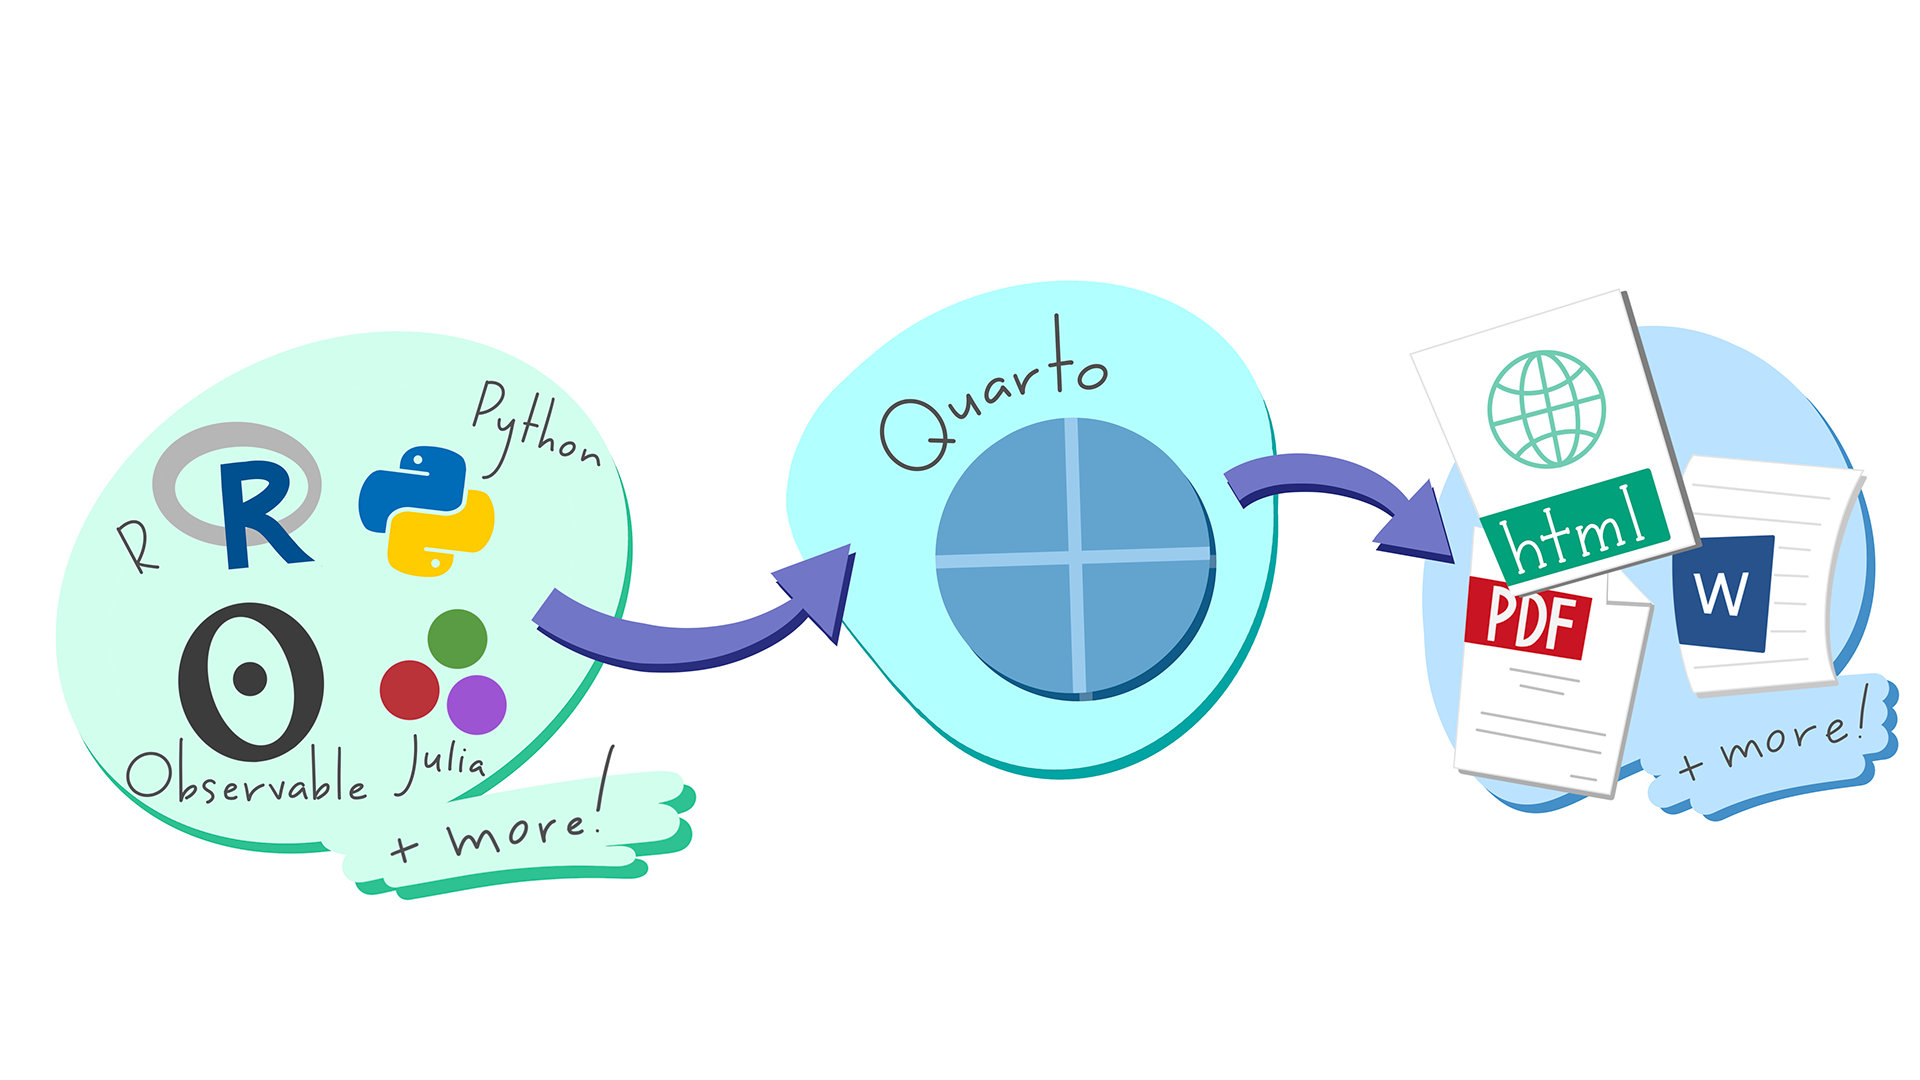
\includegraphics{img/quarto-illustration.png}}

\caption{\label{fig-quarto-illustration}Integração do Quarto}

\end{figure}%

\begin{tcolorbox}[enhanced jigsaw, opacitybacktitle=0.6, titlerule=0mm, left=2mm, toptitle=1mm, opacityback=0, arc=.35mm, colback=white, rightrule=.15mm, breakable, leftrule=.75mm, bottomrule=.15mm, colbacktitle=quarto-callout-note-color!10!white, colframe=quarto-callout-note-color-frame, coltitle=black, bottomtitle=1mm, toprule=.15mm, title=\textcolor{quarto-callout-note-color}{\faInfo}\hspace{0.5em}{O que o ChatGPT 4o nos diz sobre a Figura~\ref{fig-quarto-illustration}?}]

\begin{enumerate}
\def\labelenumi{\arabic{enumi}.}
\tightlist
\item
  \textbf{Múltiplas Linguagens de Programação}:

  \begin{itemize}
  \tightlist
  \item
    No lado esquerdo da imagem, temos ícones representando várias
    linguagens de programação e plataformas suportadas pelo Quarto,
    incluindo:

    \begin{itemize}
    \tightlist
    \item
      \textbf{R}: Linguagem popular para análise estatística e
      visualização de dados.
    \item
      \textbf{Python}: Linguagem versátil utilizada em ciência de dados,
      aprendizado de máquina, entre outras áreas.
    \item
      \textbf{Julia}: Linguagem de programação de alto desempenho para
      computação técnica.
    \item
      \textbf{Observable}: Plataforma para criar visualizações de dados
      interativas.
    \end{itemize}
  \item
    O texto ``+ more!'' indica que o Quarto suporta outras linguagens
    além das mencionadas.
  \end{itemize}
\item
  \textbf{Quarto}:

  \begin{itemize}
  \tightlist
  \item
    No centro da imagem, há um círculo azul com o logo do Quarto,
    representando a ferramenta em si.
  \item
    Quarto atua como uma plataforma de integração, permitindo que os
    usuários combinem códigos de diferentes linguagens e criem
    documentos ricos em conteúdo.
  \end{itemize}
\item
  \textbf{Exportação para Diversos Formatos}:

  \begin{itemize}
  \tightlist
  \item
    À direita, a imagem mostra os diferentes formatos para os quais o
    Quarto pode exportar:

    \begin{itemize}
    \tightlist
    \item
      \textbf{HTML}: Para visualização web.
    \item
      \textbf{PDF}: Para documentos portáteis e impressos.
    \item
      \textbf{Word (DOCX)}: Para edição e compartilhamento em formato de
      texto.
    \end{itemize}
  \item
    O texto ``+ more!'' indica que o Quarto pode exportar para outros
    formatos além dos ilustrados.
  \end{itemize}
\end{enumerate}

\end{tcolorbox}

A Figura~\ref{fig-quarto-process} explica o fluxo de trabalho de criação
e publicação de documentos com Quarto de forma mais analítica. Inicia-se
com um arquivo \texttt{.qmd} que é processado por ferramentas como knitr
ou Jupyter para gerar um arquivo Markdown. Esse arquivo Markdown é então
convertido pelo Pandoc para os formatos finais de saída, permitindo uma
ampla flexibilidade na distribuição do conteúdo.

\begin{figure}

\href{https://r-cubed-advanced.rostools.org/sessions/build-website}{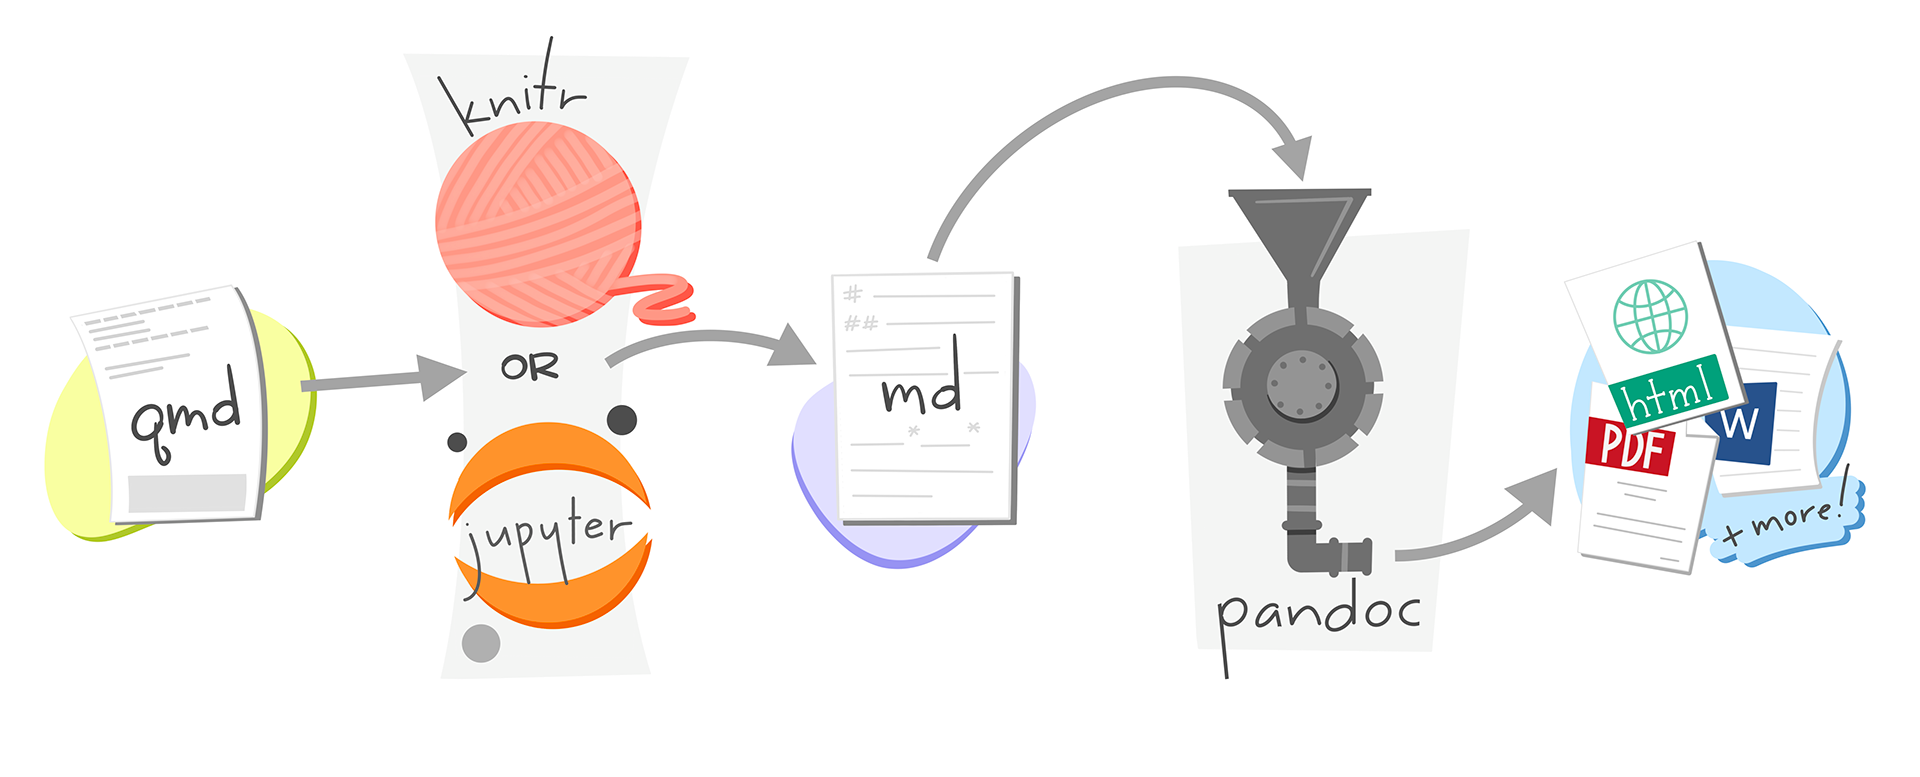
\includegraphics{img/quarto-process.png}}

\caption{\label{fig-quarto-process}Workflow analítico do Quarto}

\end{figure}%

\begin{tcolorbox}[enhanced jigsaw, opacitybacktitle=0.6, titlerule=0mm, left=2mm, toptitle=1mm, opacityback=0, arc=.35mm, colback=white, rightrule=.15mm, breakable, leftrule=.75mm, bottomrule=.15mm, colbacktitle=quarto-callout-note-color!10!white, colframe=quarto-callout-note-color-frame, coltitle=black, bottomtitle=1mm, toprule=.15mm, title=\textcolor{quarto-callout-note-color}{\faInfo}\hspace{0.5em}{O que o ChatGPT 4o nos diz sobre a Figura~\ref{fig-quarto-process}?}]

\begin{enumerate}
\def\labelenumi{\arabic{enumi}.}
\tightlist
\item
  \textbf{Documentos Quarto (qmd)}:

  \begin{itemize}
  \tightlist
  \item
    O processo começa com um documento no formato Quarto Markdown (qmd),
    que é um arquivo que pode conter texto, código e outros elementos
    dinâmicos.
  \end{itemize}
\item
  \textbf{Processamento com knitr ou Jupyter}:

  \begin{itemize}
  \tightlist
  \item
    A próxima etapa do fluxo envolve a escolha de um processador para
    converter o conteúdo do documento qmd:

    \begin{itemize}
    \tightlist
    \item
      \textbf{knitr}: Um pacote no R que permite a integração de código
      e texto, frequentemente usado para documentos R Markdown.
    \item
      \textbf{Jupyter}: Um ambiente interativo de notebooks que suporta
      várias linguagens de programação, como Python.
    \end{itemize}
  \item
    A imagem mostra que o documento \texttt{qmd} pode ser processado por
    qualquer uma dessas ferramentas, resultando em um documento Markdown
    intermediário (md).
  \end{itemize}
\item
  \textbf{Markdown (md)}:

  \begin{itemize}
  \tightlist
  \item
    Após o processamento inicial, o documento é convertido em um arquivo
    Markdown padrão (md). Este arquivo contém o texto e as marcações,
    mas ainda precisa ser convertido para o formato de saída final
    desejado.
  \end{itemize}
\item
  \textbf{Conversão com Pandoc}:

  \begin{itemize}
  \tightlist
  \item
    O arquivo Markdown é então processado pelo Pandoc, uma ferramenta
    poderosa de conversão de documentos. Pandoc é capaz de transformar
    arquivos Markdown em uma variedade de formatos de saída.
  \item
    A imagem retrata o Pandoc como uma máquina que processa o documento
    \texttt{md} e o converte para os formatos finais.
  \end{itemize}
\item
  \textbf{Formatos de Saída}:

  \begin{itemize}
  \tightlist
  \item
    O resultado final do processo pode ser exportado para diversos
    formatos, conforme ilustrado na imagem:

    \begin{itemize}
    \tightlist
    \item
      \textbf{HTML}: Para publicação na web.
    \item
      \textbf{PDF}: Para distribuição de documentos portáveis e
      impressos.
    \item
      \textbf{Word (DOCX)}: Para edição e compartilhamento em formato de
      texto.
    \end{itemize}
  \item
    Novamente, o texto ``+ more!'' indica que o Pandoc pode converter os
    documentos para outros formatos além dos mencionados.
  \end{itemize}
\end{enumerate}

\end{tcolorbox}

Se quisermos pensar o fluxo de trabalho com Quarto com enfoque
específico nos passos de criação e renderização de um documento,
oferecendo um guia passo a passo um pouco mais sintético, podemos
consider a ilustração da Figura~\ref{fig-qmd-workflow}. Essa figura
ilustra de maneira didática e sequencial as etapas que um usuário deve
seguir, desde a criação do arquivo até a renderização do documento final
em múltiplos formatos. Nessa imagem destacamos explicitamente a
incorporação e a renderização de código R, que é software mais utilizado
por pesquisadores.

\begin{figure}

\href{https://ucsbcarpentry.github.io/Reproducible-Publications-with-RStudio-Quarto/02-quarto/03-quarto-documents/index.html}{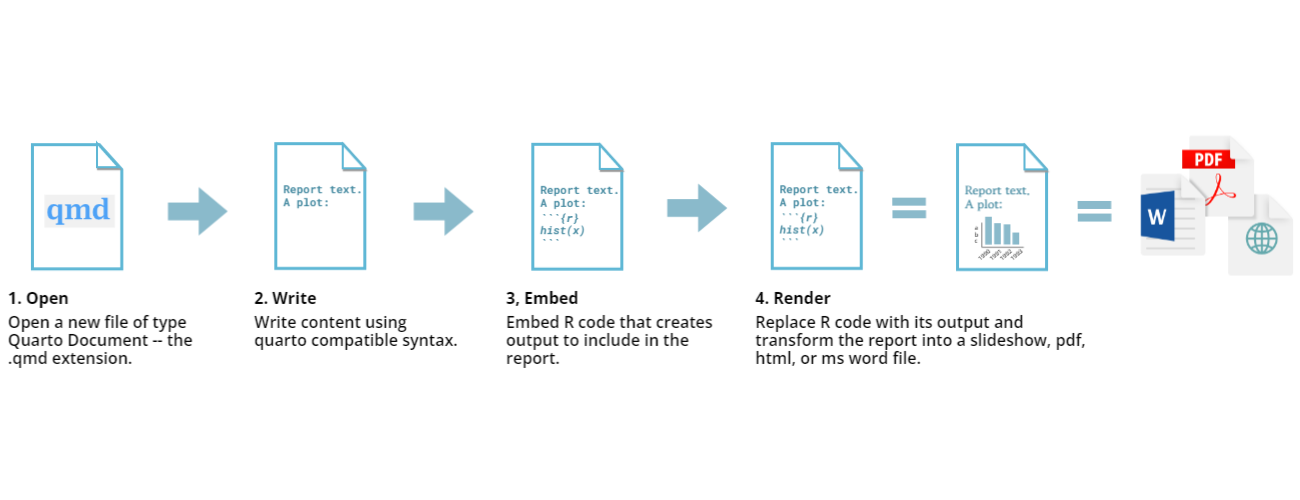
\includegraphics{img/qmd-workflow.png}}

\caption{\label{fig-qmd-workflow}Workflow sintético do Quarto}

\end{figure}%

\begin{tcolorbox}[enhanced jigsaw, opacitybacktitle=0.6, titlerule=0mm, left=2mm, toptitle=1mm, opacityback=0, arc=.35mm, colback=white, rightrule=.15mm, breakable, leftrule=.75mm, bottomrule=.15mm, colbacktitle=quarto-callout-note-color!10!white, colframe=quarto-callout-note-color-frame, coltitle=black, bottomtitle=1mm, toprule=.15mm, title=\textcolor{quarto-callout-note-color}{\faInfo}\hspace{0.5em}{O que o ChatGPT 4o nos diz sobre a Figura~\ref{fig-qmd-workflow}?}]

\begin{enumerate}
\def\labelenumi{\arabic{enumi}.}
\tightlist
\item
  \textbf{Open (Abrir)}:

  \begin{itemize}
  \tightlist
  \item
    \textbf{Passo}: Abrir um novo arquivo de tipo Quarto Document com a
    extensão \texttt{.qmd}.
  \item
    \textbf{Detalhe}: Este passo inicial foca na criação do arquivo
    fonte que será usado para todo o fluxo de trabalho subsequente.
  \end{itemize}
\item
  \textbf{Write (Escrever)}:

  \begin{itemize}
  \tightlist
  \item
    \textbf{Passo}: Escrever o conteúdo usando a sintaxe compatível com
    o Quarto.
  \item
    \textbf{Detalhe}: Este passo enfatiza a fase de escrita, onde o
    usuário insere o texto e a estrutura básica do documento.
  \end{itemize}
\item
  \textbf{Embed (Incorporar)}:

  \begin{itemize}
  \tightlist
  \item
    \textbf{Passo}: Incorporar código R que gera saída a ser incluída no
    relatório.
  \item
    \textbf{Detalhe}: Este passo mostra como os usuários podem integrar
    blocos de código no documento. Aqui, o exemplo específico de código
    R (\texttt{hist(x)}) é dado, o que ilustra a capacidade do Quarto de
    processar e renderizar código dinâmico.
  \end{itemize}
\item
  \textbf{Render (Renderizar)}:

  \begin{itemize}
  \tightlist
  \item
    \textbf{Passo}: Substituir o código R pela sua saída e transformar o
    relatório em uma apresentação de slides, PDF, HTML ou arquivo MS
    Word.
  \item
    \textbf{Detalhe}: Este passo final detalha o processo de
    renderização, onde o Quarto processa o código embutido, gera os
    resultados e cria o documento final no formato desejado.
  \end{itemize}
\end{enumerate}

\end{tcolorbox}

E por fim, se desejamos melhorar nosso entendimento de como utilizar o
Quarto no contexto de uma pesquisa científica empírica, a
Figura~\ref{fig-all-workflow} enfatiza a integração da narrativa
científica, código e dados, culminando na publicação de resultados. Esse
fluxo de trabalho é ideal para pesquisas que requerem transparência e
reprodutibilidade, permitindo que outros pesquisadores verifiquem e
repliquem os resultados. A integração da narrativa científica, código e
dados em um único documento facilita a manutenção e a atualização do
trabalho. Além disso, a capacidade de publicar tanto em formatos
estáticos quanto dinâmicos amplia o alcance e o impacto da pesquisa,
atendendo a diferentes necessidades de distribuição e engajamento do
público.

\begin{figure}

\href{https://towardsdatascience.com/technical-writing-and-publishing-data-rich-articles-with-quarto-d61a56bcaa64}{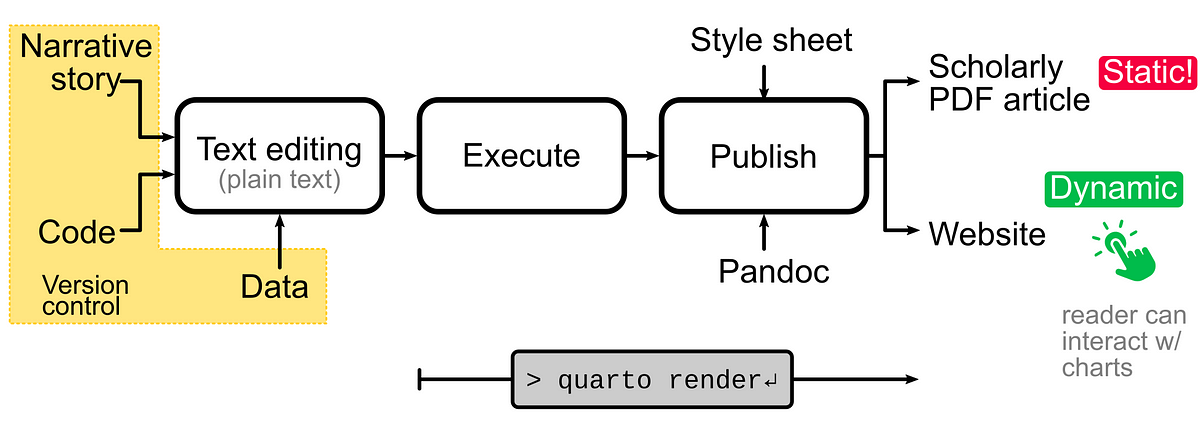
\includegraphics{img/all-workflow.png}}

\caption{\label{fig-all-workflow}Workflow de uma pesquisa empírica
utilizando Quarto}

\end{figure}%

\begin{tcolorbox}[enhanced jigsaw, opacitybacktitle=0.6, titlerule=0mm, left=2mm, toptitle=1mm, opacityback=0, arc=.35mm, colback=white, rightrule=.15mm, breakable, leftrule=.75mm, bottomrule=.15mm, colbacktitle=quarto-callout-note-color!10!white, colframe=quarto-callout-note-color-frame, coltitle=black, bottomtitle=1mm, toprule=.15mm, title=\textcolor{quarto-callout-note-color}{\faInfo}\hspace{0.5em}{O que o ChatGPT 4o nos diz sobre a Figura~\ref{fig-all-workflow}?}]

\begin{enumerate}
\def\labelenumi{\arabic{enumi}.}
\tightlist
\item
  \textbf{Narrativa e Código (Narrative story, Code, Data)}:

  \begin{itemize}
  \tightlist
  \item
    \textbf{Narrativa}: A história ou o contexto da pesquisa, incluindo
    introdução, metodologia, resultados e discussão, é escrita em texto
    plano.
  \item
    \textbf{Código}: O código utilizado para análises, simulações ou
    geração de figuras e tabelas. Esse código pode ser gerido através de
    controle de versão, garantindo rastreabilidade e reprodutibilidade.
  \item
    \textbf{Dados}: Os dados brutos ou processados usados na pesquisa,
    que também podem estar sob controle de versão.
  \end{itemize}
\item
  \textbf{Edição de Texto (Text editing)}:

  \begin{itemize}
  \tightlist
  \item
    \textbf{Edição de Texto Plano}: A narrativa e o código são
    combinados em um editor de texto plano, formando um documento
    integral que contém a descrição da pesquisa e os scripts de análise.
  \end{itemize}
\item
  \textbf{Execução (Execute)}:

  \begin{itemize}
  \tightlist
  \item
    \textbf{Executar Código}: O código embutido no documento é
    executado, gerando saídas como gráficos, tabelas e resultados
    estatísticos que são automaticamente incorporados ao documento.
  \end{itemize}
\item
  \textbf{Publicação (Publish)}:

  \begin{itemize}
  \tightlist
  \item
    \textbf{Folha de Estilo (Style sheet)}: Um template pode ser
    aplicado para formatar o documento de acordo com as normas de
    publicação ou preferências estilísticas.
  \item
    \textbf{Pandoc}: Ferramenta usada para converter o documento em
    vários formatos de saída.
  \item
    \textbf{Resultados}:

    \begin{itemize}
    \tightlist
    \item
      \textbf{Artigo PDF Estático (Scholarly PDF article)}: Um documento
      PDF pronto para submissão a revistas acadêmicas ou para
      distribuição formal. É um formato estático, onde o conteúdo é fixo
      e não interativo.
    \item
      \textbf{Website Dinâmico (Website)}: Um site interativo onde os
      leitores podem interagir com gráficos e visualizações de dados.
      Este formato permite uma experiência de leitura mais envolvente.
    \end{itemize}
  \end{itemize}
\item
  \textbf{Renderização (quarto render)}:

  \begin{itemize}
  \tightlist
  \item
    \textbf{Comando de Renderização}: O comando \texttt{quarto\ render}
    é utilizado para processar o documento (projeto) e gerar as versões
    finais nos formatos desejados.\vspace{0.5em}
  \end{itemize}
\end{enumerate}

\textbf{Fluxo de Trabalho de uma Pesquisa Empírica
Hipotética}:\vspace{0.5em}

\begin{enumerate}
\def\labelenumi{\arabic{enumi}.}
\tightlist
\item
  \textbf{Início}:

  \begin{itemize}
  \tightlist
  \item
    Começa com a escrita da narrativa da pesquisa e o desenvolvimento do
    código para análise dos dados.
  \item
    Os dados são coletados e preparados, podendo ser versões controladas
    para assegurar integridade e reprodutibilidade.
  \end{itemize}
\item
  \textbf{Edição e Integração}:

  \begin{itemize}
  \tightlist
  \item
    O texto da narrativa, o código e os dados são integrados em um único
    documento Quarto (.qmd), utilizando um editor de texto plano.
  \end{itemize}
\item
  \textbf{Execução de Análises}:

  \begin{itemize}
  \tightlist
  \item
    O código é executado dentro do documento, gerando os resultados das
    análises que são automaticamente incorporados à narrativa.
  \end{itemize}
\item
  \textbf{Preparação para Publicação}:

  \begin{itemize}
  \tightlist
  \item
    Aplicação de um template para garantir que o documento final esteja
    formatado corretamente.
  \item
    Uso do Pandoc para converter o documento em formatos de saída, tanto
    estáticos (PDF) quanto dinâmicos (site web interativo).
  \end{itemize}
\item
  \textbf{Publicação e Distribuição}:

  \begin{itemize}
  \tightlist
  \item
    \textbf{PDF Estático}: Criado para ser submetido a revistas
    científicas ou compartilhado formalmente.
  \item
    \textbf{Website Dinâmico}: Disponibilizado para o público,
    permitindo interação com os dados e gráficos, promovendo maior
    engajamento e entendimento dos resultados da pesquisa.
  \end{itemize}
\end{enumerate}

\end{tcolorbox}

\bookmarksetup{startatroot}

\chapter{Controle de Ambiente}\label{sec-docker}

Imagine a seguinte situação: você publicou uma pesquisa quantitativa,
disponibilizando o código e os dados para que outros pesquisadores
possam reproduzir os resultados. Um pesquisador entra em contato e diz
que não conseguiu replicar seus resultados. Você como bom mineiro,
responde: ``Uai, comigo funcionou!''. Prestativo como é sugere para o
pesquisador, da Polônia, que venha até sua casa para que você possa
ajudá-lo, e aproveitar para tomar um café e comer um pão de queijo. O
pesquisador, educadamente, responde que não pode ir até sua casa, pois
está do outro lado do mundo.

Então, prestativo como é, você sugere que vai enviar uma imagem do seu
HD para ele. O pesquisador, educadamente, responde que não pode aceitar,
pois o arquivo da imagem é muito grande e ele não tem espaço suficiente
para armazenar a imagem. Além do mais, ele não entende muito bem (e não
tem!) a infraestrutura para pode acessar seu HD. Inclusive, ele utiliza
um sistema operacional (e estrutura de hardware) diferente do seu.

Pois bem, essa situação poderia ser a única saída alguns anos atrás. No
entanto, hoje em dia, com os serviços de armazenamento em nuvem, as
soluções de virtualização (máquinas virtuais), containers e controle de
ambiente, é possível compartilhar o ambiente de desenvolvimento de forma
mais simples.

Máquinas virtuais (VM) são ambientes que emulam um sistema operacional
(SO) completo sobre um hardware físico, permitindo a execução de
múltiplos sistemas operacionais em uma única máquina. Elas oferecem um
alto nível de isolamento e controle, pois cada VM inclui seu próprio SO,
bibliotecas e aplicativos. As VMs podem ser classificadas em dois tipos:
\emph{Type 1 Hypervisor} e \emph{Type 2 Hypervisor}. Tipo 1 Hypervisor
roda diretamente sobre o hardware, gerenciando várias VMs sem a
necessidade de um SO subjacente, o que proporciona melhor desempenho e
eficiência. Já o \emph{Type 2 Hypervisor} roda sobre um SO existente,
sendo menos eficiente, mas mais fácil de configurar e utilizar em
ambientes de desktop Figura~\ref{fig-vm-container}.

\begin{figure}

\centering{

\href{https://doi.org/10.5281/zenodo.12521134}{\includegraphics{img/vm-container.png}}

}

\caption{\label{fig-vm-container}Soluções para controle do ambiente de
desenvolvimento. Ilustração disponível em:
https://doi.org/10.5281/zenodo.12521134}

\end{figure}%

Exemplos de soluções de virtualização Tipo 1 podemos elencar:

\begin{itemize}
\item
  \href{https://www.vmware.com/products/esxi-and-esx.html.html}{\textbf{VMware
  ESXi}}: Uma solução comercial amplamente utilizada em ambientes
  corporativos para criar e gerenciar VMs. Oferece alta performance e
  várias funcionalidades avançadas de gerenciamento.
\item
  \href{https://learn.microsoft.com/pt-br/windows-server/virtualization/hyper-v/hyper-v-technology-overview}{\textbf{Microsoft
  Hyper-V}}: Integrado ao Windows, é uma solução comercial que também
  pode ser usada gratuitamente com recursos limitados. Hyper-V é
  amplamente utilizado em ambientes Windows.
\item
  \href{https://xenproject.org/}{\textbf{Xen}:} Uma solução open-source
  popular em ambientes de nuvem, como o Amazon Web Services (AWS). Xen é
  altamente eficiente e suportado por várias distribuições Linux.
\end{itemize}

Exemplos de Tipo 2 incluem:

\begin{itemize}
\item
  \href{https://www.vmware.com/products/desktop-hypervisor.html}{\textbf{VMware
  Workstation}}: Uma solução comercial usada principalmente em desktops
  e laptops para executar múltiplos SOs. VMware Workstation é conhecido
  pela sua estabilidade e facilidade de uso. Recentemente ele passou a
  ser gratuito.
\item
  \href{https://www.virtualbox.org/}{\textbf{Oracle VirtualBox}}: Uma
  solução open-source amplamente utilizada para virtualização em
  desktops. VirtualBox é gratuito e suporta uma vasta gama de SOs
  convidados.
\item
  \href{https://www.parallels.com/br/}{\textbf{Parallels Desktop}}: Uma
  solução comercial popular entre usuários de Mac, permitindo que eles
  rodem Windows, Linux e outros no macOS de maneira integrada.
\end{itemize}

As vantagens das VMs incluem um alto isolamento e segurança, além da
flexibilidade para rodar diferentes SOs. No entanto, elas consomem
muitos recursos, como CPU, memória e armazenamento, e as imagens são
grandes e difíceis de compartilhar (Clyburne-Sherin et al., 2019). Nesse
sentido, para a reprodutibilidade das pesquisas empíricas no ambito da
Ciência Aberta o emprego de VMs pode ser impraticável. Para nosso dia a
dia enquanto pesquisadores e professores pode ser uma ferramenta
extremamente últil. \textbf{Esse curso está organizado dentro de uma
VM}.

Por outro lado, os containers são uma tecnologia de virtualização a
nível de SO, mais leve que as VMs, que compartilham o mesmo kernel do SO
hospedeiro, mas ainda assim oferecem isolamento para aplicações.
\href{https://www.docker.com/}{Docker},
\href{https://kubernetes.io/}{Kunernetes} e
\href{https://www.redhat.com/en/technologies/cloud-computing/openshift}{OpenShift}
são uma das ferramentas mais populares para criar e gerenciar
containers. Ao contrário das VMs, os containers contêm apenas a
aplicação e suas dependências, compartilhando o kernel do SO hospedeiro.
Isso torna os containers mais leves e eficientes em termos de recursos,
e ainda são rápidos na inicialização e execução. Além disso, são fáceis
de distribuir e compartilhar (Clyburne-Sherin et al., 2019).

Enquanto as VMs oferecem maior isolamento, os containers têm menor
consumo de recursos e são mais práticos para desenvolvimento e
distribuição de aplicações. No entanto, eles compartilham o kernel do SO
hospedeiro, o que resulta em menor isolamento comparado às VMs. Os
contêineres estão ganhando força na pesquisa científica (Moreau et al.,
2023) e o Docker despontado como uma das soluções mais populares para
controle de ambiente em pesquisas empíricas quantitativas (Wiebels \&
Moreau, 2021).

Por fim, temos as ferramentas de controle de ambiente como
\href{https://docs.conda.io/projects/conda/en/stable/}{Conda} e
\href{https://rstudio.github.io/renv/articles/renv.html}{renv}, que
ajudam a gerenciar pacotes e dependências em ambientes de
desenvolvimento, sem a necessidade de virtualização. Conda, por exemplo,
gerencia pacotes, dependências e ambientes virtuais para linguagens como
Python e R, permitindo criar ambientes isolados com versões específicas
de pacotes e dependências. Já o renv (R Environment) é específico para
projetos R, criando um ambiente de desenvolvimento reproduzível.

Essas ferramentas oferecem a vantagem de menor sobrecarga de recursos e
são fáceis de configurar e utilizar, promovendo a reprodutibilidade de
ambientes de desenvolvimento para linguagens específicas. No entanto,
oferecem menor isolamento comparado às VMs e containers e dependem da
compatibilidade do sistema operacional e das versões dos pacotes.

A recomendação para os pesquisadores que desejem terem seus trabalhos
transparentes e reprodutíveis é que eles entendam das duas últimas
soluções, por exemplo, num ambiente R, de containers + renv. Na verdade,
essas duas soluções devem caminhar juntas, pois no contexto da maioria
dos workflows (pipelines) de pesquisa a construção de containers é
facilitada pela aplicação correta dos pacotes de controle de ambiente
(Conda, renv, etc.).

No entanto, a computação em nuvens também nos agraciou com outras
soluções que facilitam a reprodutibilidade, transparência e colaboração
em pesquisas empíricas. Plataformas de notebooks na nuvem como
\href{https://colab.research.google.com/}{Google Colab} e
\href{https://posit.cloud/}{Posit Cloud} (anteriormente conhecido como
RStudio Cloud) permitem compartilhar notebooks rodando num mesmo
hardware, mas os usuários precisam garantir que as dependências e
versões de pacotes sejam corretamente especificadas e gerenciadas.

No \href{https://jupyter.org/hub}{JupyterHub} temos proposta parecida,
mas ele nos dá um controle melhor sobre o ambiente, já que um
administrador pode configurar e manter as dependências necessárias de um
projeto colaborativo. O \href{https://mybinder.org/}{Binder} é uma
plataforma open-source que transforma repositórios Git em ambientes
executáveis, focando principalmente em notebooks Jupyter. Ele facilita a
execução de notebooks a partir de repositórios Git e garante que as
dependências especificadas no repositório sejam instaladas, mas depende
da configuração correta dos arquivos de dependências.

O \href{https://codeocean.com/}{Code Ocean} e
\href{https://nextjournal.com/}{Nextjournal} são soluções específicas
para a reprodutibilidade de pesquisas científicas, focando na facilidade
de uso e na acessibilidade para a comunidade acadêmica. O Code Ocean
permite que os cientistas agrupem código, dados, resultados, metadados e
um ambiente computacional em um único lugar --- chamado de ``cápsula'',
cujos resultados podem ser reproduzidos por qualquer pessoa num simples
botão (Clyburne-Sherin et al., 2019). O Nextjournal é uma plataforma de
colaboração e publicação de notebooks interativos, que permite a
execução de código em diferentes linguagens, como o Code Ocean, e a
criação de artigos científicos interativos. Essas duas soluções oferecem
um ambiente integrado, com interface gráfica intuitiva para configurar
ambientes de desenvolvimento e execução, o que facilita para
pesquisadores sem conhecimento técnico avançado. No entanto, são
soluções comerciais e podem ter limitações em termos de recursos e
personalização.

As soluções apresentadas sobrepostas à nuvem do lado direito na
Figura~\ref{fig-vm-container} podem ser consideradas soluções
intermediárias aos containers tradicionais, no sentido de que elas
utilizam conteinerização para criar ambientes reprodutíveis, mas
abstraem a complexidade técnica e fornecem interfaces mais amigáveis e
específicas para a comunidade científica. Elas são ideais para
pesquisadores que buscam simplicidade e reprodutibilidade sem a
necessidade de se aprofundar nos detalhes técnicos dos containers. Essas
plataformas tornam a poderosa tecnologia de conteinerização acessível e
aplicável ao contexto da pesquisa científica.

Podemos dizer que em termos de níveis de reprodutibilidade, Google Colab
e Posit Cloud atendem a um nível básico, porque a reprodutibilidade pode
ser limitada pela variabilidade das dependências das sessões e cabe ao
usuário uma configuração cuidadosa dos pacotes e versões. Binder e
JupyterHub fornecem um nível intermediário de reprodutibilidade, pois
apesar de um melhor controle sobre o ambiente, requer configuração e
manutenção adequadas das dependências. Por fim, Code Ocean e Nextjournal
oferecem um alto nível de reprodutibilidade, pois são ambientes
integrados para criar, executar e compartilhar projetos de pesquisa
reprodutíveis.

\begin{tcolorbox}[enhanced jigsaw, opacitybacktitle=0.6, titlerule=0mm, left=2mm, toptitle=1mm, opacityback=0, arc=.35mm, colback=white, rightrule=.15mm, breakable, leftrule=.75mm, bottomrule=.15mm, colbacktitle=quarto-callout-note-color!10!white, colframe=quarto-callout-note-color-frame, coltitle=black, bottomtitle=1mm, toprule=.15mm, title=\textcolor{quarto-callout-note-color}{\faInfo}\hspace{0.5em}{\emph{Leveraging Containers for Reproducible Psychological Research}
(Tip~\ref{tip-prompt})}]

O artigo de Wiebels \& Moreau (2021) discute a importância e a aplicação
das práticas de ciência aberta na pesquisa. Eles destacam que, desde
2019, cerca de 35\% dos pesquisadores de psicologia adotaram práticas de
CA, um aumento significativo em relação aos 5\% de apenas cinco anos
antes.\vspace{0.5em}

O artigo, inicialmente, discute o pacote
\href{https://rstudio.github.io/renv/articles/renv.html}{renv}, que
gerencia dependências em R armazenando o código-fonte de todos os
pacotes R usados em um projeto. No entanto, eles observam que essa
abordagem não lida com dependências do sistema ou dependências de outras
linguagens de programação e pacotes de software.\vspace{0.5em}

Para resolver essas limitações, os autores apresentam os ``containers'',
que permitem empacotar todo o código e dependências para garantir que as
análises sejam executadas de maneira confiável em uma variedade de
sistemas operacionais e versões de software. Eles descrevem a lógica por
trás dos containers, o que são e os problemas práticos que podem
resolver.\vspace{0.5em}

Os autores explicam que o ideal é ``empacotar'' (isolar) todo o ambiente
de computação de forma que qualquer pessoa em qualquer computador possa
examinar e replicar nosso trabalho, independentemente do software
instalado, drivers e sistemas operacionais. Uma maneira popular de
alcançar esse objetivo é com máquinas virtuais (VMs), mas as VMs podem
ficar muito grandes e lentas, o que pode tornar o compartilhamento e o
uso delas impraticáveis. Os containers também isolam ambientes de
computação, mas usam menos recursos do que as VMs.\vspace{0.5em}

Apesar de suas vantagens, a contêinerização ainda é raramente usada na
psicologia, talvez por falta de conscientização ou porque o uso - e
especialmente a construção - de containers pode parecer assustador para
aqueles que não têm formação em ciência da computação. Para superar essa
barreira, os autores usam a plataforma de contêiner
\href{https://www.docker.com/}{Docker} e se concentram na linguagem
R.\vspace{0.5em}

Eles explicam que o Docker é um projeto de contêinerização de código
aberto baseado em Linux; ou seja, o Linux está rodando dentro dos
containers, mesmo que estejamos em um computador Windows ou Mac. Eles
também esclarecem que um número ilimitado de containers pode ser criado
a partir de uma imagem e, ao contrário das imagens, os containers podem
ser modificados enquanto estão em execução.\vspace{0.5em}

Os autores comparam uma imagem Docker a uma receita de bolo e o
container Docker correspondente a um bolo acabado. A receita contém as
instruções para fazer o bolo, pode ser usada para fazer quantos bolos
você quiser e pode ser compartilhada para permitir que outros façam o
mesmo bolo. Todos que usam a receita acabam com o mesmo tipo de bolo,
que pode ser modificado adicionando, por exemplo, cobertura ou
confeites. No entanto, sua adição de cobertura e minha adição de
confeites não mudarão a receita, e da próxima vez que usarmos a receita,
teremos o mesmo bolo de antes.\vspace{0.5em}

Os autores escolheram usar o Docker para o tutorial por cinco razões
principais. Primeiro, o Docker é uma das principais plataformas de
contêiner e foi estabelecido como uma prática recomendada em vários
campos de pesquisa. Segundo, o Docker funciona em todos os principais
sistemas operacionais (Linux, macOS e Windows). Terceiro, os containers
Docker são fáceis de usar, muito leves e rápidos. Quarto, as imagens
Docker podem ser armazenadas e compartilhadas gratuitamente no registro
central Docker Hub. Finalmente, graças à sua crescente popularidade, o
Docker se beneficia de uma grande comunidade de usuários e um rico
ecossistema de ferramentas relacionadas, como o Rocker, que fornece
containers com ambientes R.\vspace{0.5em}

Os autores concluem que a contêinerização é um passo importante para
tornar a pesquisa reprodutível, fornecendo um ambiente de computação
consistente que pode ser usado por todos os colaboradores ao longo do
projeto e que pode ser compartilhado junto com a publicação.
Compartilhar um container após a finalização de um projeto de pesquisa
garante que suas análises sejam reprodutíveis. Nesse contexto, a
proficiência em contêinerização, entre o conjunto mais amplo de
ferramentas computacionais exigidas por um cientista moderno, pode se
revelar um investimento valioso para cientistas comportamentais em todos
os estágios de carreira.

\end{tcolorbox}

\bookmarksetup{startatroot}

\chapter{IA Aplicada à Pesquisa Científica}\label{sec-AI}

Nesta última aula discutiremos o papel da inteligência artificial (IA)
na pesquisa científica, com ênfase em como essas tecnologias podem ser
integradas a práticas de ciência aberta. A IA oferece ferramentas para a
análise da literatura, fichamento, identificação de problemas de
pesquisa, lacuna, escrita e muito mais. Algumas plataformas que
discutiremos: Semantic Scholar, Research Rabbit e Inciteful. Além disso,
abordaremos ferramentas como Scholarcy que oferece resumos automáticos e
explicações detalhadas de artigos científicos, tornando o processo de
revisão e compreensão da literatura mais eficiente. Com essas
tecnologias, podemos dedicar mais tempo ao desenvolvimento de hipóteses
e à análises, enquanto a IA cuida da análise preliminar e da organização
de dados.

Vamos explorar essas ferramentas e discutir como elas podem ser
aplicadas aos nossos próprios projetos de pesquisa, promovendo uma
abordagem mais aberta, colaborativa e eficiente na ciência.

\begin{tcolorbox}[enhanced jigsaw, opacitybacktitle=0.6, titlerule=0mm, left=2mm, toptitle=1mm, opacityback=0, arc=.35mm, colback=white, rightrule=.15mm, breakable, leftrule=.75mm, bottomrule=.15mm, colbacktitle=quarto-callout-note-color!10!white, colframe=quarto-callout-note-color-frame, coltitle=black, bottomtitle=1mm, toprule=.15mm, title=\textcolor{quarto-callout-note-color}{\faInfo}\hspace{0.5em}{Transcrição de uma das palestras do Prof.~Ricardo Limongi}]

Na lista de vídeos indicados em nossa Agenda temos uma recente
\href{https://youtu.be/-WBfK9V1-ZE?si=Usd0KdyeJvoVmQ05}{palestra do
Prof.~Ricardo Limongi} sobre o uso de IA na pesquisa científica. Em
cerca de duas horas o professor abordou o uso prático, questões éticas,
ferramentas e reflexões sobre IA e métodos de síntese de conhecimento
com o Grupo PBE-USP.\vspace{0.5em}

Podemos utilizar alguma ferramenta de IA para nos ajudar a entender o
enrendo e tópicos da palestra? Pois bem, fomos no Youtube, copiamos a
transcrição da palestra, e depois utilizamos o
\href{https://aistudio.google.com}{AI Studio do Google} com a seguinte
prompt:\vspace{0.5em}

\emph{O texto abaixo é a transcrição de uma aula sobre Ferramentas de IA
aplicadas à Pesquisa Científica. Gostaria que elencasse os pontos
abordados nesse vídeo.}\vspace{0.5em}

\textbf{OBS:} Não colamos a transcrição aqui devido a quantidade de
palavras (2 horas de palestra!). Inclusive, por esse motivo, utilizamos
\href{https://aistudio.google.com}{AI Studio do Google}, que na sua
versão teste aceita um milhão de tokens.\vspace{0.5em}

Eis a resposta:\vspace{0.5em}

\textbf{Pontos abordados na aula sobre Ferramentas de IA aplicadas à
Pesquisa Científica:}\vspace{0.5em}

\textbf{1. Introdução e Apresentação:}\vspace{0.5em}

\begin{itemize}
\tightlist
\item
  Apresentação do grupo de pesquisa de prática baseada em evidências na
  saúde e dos palestrantes.
\item
  Breve currículo do professor Ricardo Limongi, especialista em
  Inteligência Artificial e marketing.
\item
  Ênfase na importância de compartilhar conhecimento e ser generoso
  dentro da comunidade acadêmica.\vspace{0.5em}
\end{itemize}

\textbf{2. Inteligência Artificial como Meio e não Fim:}\vspace{0.5em}

\begin{itemize}
\tightlist
\item
  Discussão sobre a rápida ascensão da IA e a necessidade de
  aprendizado, especialmente após o lançamento do ChatGPT.
\item
  Alerta sobre o uso excessivo da IA como ferramenta para gerar artigos
  completos, enfatizando que a IA deve ser vista como uma ferramenta
  auxiliar e não substituir o papel do pesquisador.
\item
  Importância da reflexão crítica e da capacidade de análise e
  interpretação do ser humano.\vspace{0.5em}
\end{itemize}

\textbf{3. Ciência Aberta e Replicação:}\vspace{0.5em}

\begin{itemize}
\tightlist
\item
  Discussão sobre o movimento de ciência aberta e sua importância para a
  replicabilidade de pesquisas.
\item
  Ênfase na transparência, compartilhamento de dados e o escrutínio
  crítico na comunidade científica.
\item
  Menção a plataformas como ``ArXiv'' para disponibilização de materiais
  para avaliação e crítica.\vspace{0.5em}
\end{itemize}

\textbf{4. Inteligência Artificial como Automação de
Tarefas:}\vspace{0.5em}

\begin{itemize}
\tightlist
\item
  Conceituação da IA como ferramenta de automação de tarefas, desde a
  revisão da literatura à análise de dados.
\item
  Apresentação de plataformas de IA categorizadas por tipo de tarefa e
  de diferentes modelos de acesso (gratuitas e pagas).
\item
  Menção ao crescimento do mercado da IA e à necessidade de recursos
  para acesso a plataformas mais avançadas.\vspace{0.5em}
\end{itemize}

\textbf{5. A Importância da Organização e Transparência na
Pesquisa:}\vspace{0.5em}

\begin{itemize}
\tightlist
\item
  Discussão sobre a necessidade de organização do processo de pesquisa
  desde o início, incluindo declaração de hipóteses, objetivos e
  metodologia.
\item
  Importância da clareza nas informações fornecidas à IA para evitar
  vieses e garantir a qualidade do resultado.
\item
  Críticas à falta de transparência na metodologia de alguns artigos,
  dificultando a replicação e o aprendizado da IA.
\item
  Sugestão de incluir informações sobre o uso de IA na sessão de métodos
  dos artigos para promover transparência e aprendizado.\vspace{0.5em}
\end{itemize}

\textbf{6. Ferramentas de IA para Revisão da Literatura:}\vspace{0.5em}

\begin{itemize}
\tightlist
\item
  Apresentação do Semantic Scholar como ferramenta de busca e análise de
  literatura, e sua integração com plataformas como o Google Scholar e o
  LitMaps.
\item
  Demonstração do LitMaps como plataforma para revisão da literatura com
  interface visual, recursos de fichamento e funcionalidades para
  identificar estudos similares.
\item
  Menção à plataforma ``Research Gate'' como rede social para
  pesquisadores e sua limitação em relação à publicação de artigos.
\item
  Sugestão de criar perfis nas plataformas de IA para beneficiar do
  aprendizado personalizado do algoritmo.
\item
  Explicação do recurso ``TLDR'' (Too Long, Didn't Read) como resumo do
  resumo para facilitar a análise inicial de artigos.\vspace{0.5em}
\end{itemize}

\textbf{7. Ferramentas de IA para Detecção de Plágio e Uso da
IA:}\vspace{0.5em}

\begin{itemize}
\tightlist
\item
  Diferenciação entre plágio e uso de IA na escrita, e a necessidade de
  entender o contexto e o percentual de similaridade para identificar
  possíveis problemas.
\item
  Apresentação de ferramentas de detecção de IA em textos como o
  ``Detector de IA'', disponível no LitMaps.
\item
  Discussão sobre a tolerância ao uso da IA na escrita, e a necessidade
  de diretrizes para a utilização ética e transparente.
\item
  Sugestão de submeter tanto a versão humana quanto a versão editada
  pela IA para a avaliação dos editores.\vspace{0.5em}
\end{itemize}

\textbf{8. Ferramentas de IA para Análise de Dados:}\vspace{0.5em}

\begin{itemize}
\tightlist
\item
  Demonstração do ``Consensus'' como ferramenta para analisar e avaliar
  relações entre variáveis, utilizando dados do Semantic Scholar.
\item
  Apresentação do CoPilot como recurso de interação com os dados e
  geração de insights.
\item
  Discussão sobre a importância de entender os algoritmos e a capacidade
  de interpretação crítica dos resultados da IA.\vspace{0.5em}
\end{itemize}

\textbf{9. Desafios e Limitações da IA na Pesquisa:}\vspace{0.5em}

\begin{itemize}
\tightlist
\item
  Discussão sobre a questão da privacidade de dados e os riscos de
  vazamento de informações confidenciais ao utilizar plataformas de IA.
\item
  Menção ao Microsoft CoPilot como alternativa com maior segurança de
  dados.
\item
  Alerta sobre a falta de leitura dos termos de uso e a necessidade de
  atenção para a proteção de dados sensíveis.
\item
  Discussão sobre a dificuldade de rastrear e evitar o uso indevido da
  IA em pareceres e trabalhos acadêmicos.
\item
  Menção ao problema da falta de acesso a conteúdos científicos pagos,
  limitando o aprendizado da IA e criando desigualdade de acesso.
\item
  Ênfase na necessidade de acesso aberto a artigos científicos para
  facilitar o aprendizado e democratizar o acesso à
  informação.\vspace{0.5em}
\end{itemize}

\textbf{10. Letramento Digital e a Importância do Ensino da
IA:}\vspace{0.5em}

\begin{itemize}
\tightlist
\item
  Discussão sobre a importância do letramento digital e da educação para
  o uso ético e responsável da IA na pesquisa.
\item
  Ênfase na necessidade de repensar as disciplinas de metodologia e
  integrar o ensino da IA de forma crítica e consciente.
\item
  Compartilhamento de exemplos de iniciativas de letramento digital para
  professores e pesquisadores, como o ``Academia GPT''.
\item
  Alerta sobre a necessidade de desenvolver habilidades para identificar
  o uso indevido da IA e avaliar criticamente os resultados.
\item
  Ênfase na importância de entender os processos de pesquisa e os
  fundamentos da metodologia para utilizar a IA de forma eficiente e
  ética.\vspace{0.5em}
\end{itemize}

\textbf{11. Conclusões e Considerações Finais:}\vspace{0.5em}

\begin{itemize}
\tightlist
\item
  Reconhecimento da IA como ferramenta fundamental para a pesquisa, mas
  com a necessidade de uso consciente e responsável.
\item
  Importância de desenvolver um letramento digital para a pesquisa, com
  foco na ética, na crítica e na interpretação.
\item
  Incentivo à participação em debates e à criação de diretrizes para o
  uso da IA na pesquisa.
\item
  Ênfase na necessidade de adaptação do ensino da metodologia para
  incorporar o uso da IA de forma crítica e consciente.
\item
  Reconhecimento da importância do conhecimento e da expertise humana
  para a análise e interpretação dos resultados da IA.\vspace{0.5em}
\end{itemize}

Em suma, a aula abordou a utilização da IA como ferramenta auxiliar na
pesquisa científica, destacando sua potencialidade e os desafios para
seu uso ético e responsável. A principal mensagem é que a IA deve ser
integrada ao processo de pesquisa como um complemento e não como um
substituto, sendo crucial o desenvolvimento de um letramento digital
para o uso crítico e consciente da ferramenta.

\end{tcolorbox}

\bookmarksetup{startatroot}

\chapter*{Referências}\label{referuxeancias}
\addcontentsline{toc}{chapter}{Referências}

\markboth{Referências}{Referências}

\phantomsection\label{refs}
\begin{CSLReferences}{1}{0}
\bibitem[\citeproctext]{ref-albano2023}
Albano, C. S., Pedroso, P. de O., \& Caetano, D. O. (2023). Ci{ê}ncia
{Aberta}: {Um Panorama} Sobre as {Publica{ç}{õ}es} No {Cen{á}rio
Brasileiro}. \emph{Saber Cient{í}fico}, \emph{12}(1), 1--12.

\bibitem[\citeproctext]{ref-baker2023}
Baker, D. H., Berg, M., Hansford, K., Quinn, B. P. A., Segala, F. G., \&
English, E. (2023). \emph{{ReproduceMe}: Lessons from a Pilot Project on
Computational Reproducibility} {[}Preprint{]}. PsyArXiv.
\url{https://doi.org/10.31234/osf.io/k8d4u}

\bibitem[\citeproctext]{ref-baker2016}
Baker, M. (2016). 1,500 Scientists Lift the Lid on Reproducibility.
\emph{Nature}, \emph{533}(7604), 452--454.
\url{https://doi.org/10.1038/533452a}

\bibitem[\citeproctext]{ref-prashantakumarbehera2023}
Behera, P. K., \& Jain, S. J. (2023). \emph{Zotero -- An Open-Source
Reference Management Software: A Practical Manual}. OSF.
\url{https://doi.org/10.17605/OSF.IO/8S73R}

\bibitem[\citeproctext]{ref-bernard2023}
Bernard, C. (2023). Stop {Reproducing} the {Reproducibility Crisis}.
\emph{Eneuro}, \emph{10}(2), ENEURO.0032--23.2023.
\url{https://doi.org/10.1523/ENEURO.0032-23.2023}

\bibitem[\citeproctext]{ref-bezjak2018}
Bezjak, S., Clyburne-Sherin, A., Conzett, P., Fernandes, P., Görögh, E.,
Helbig, K., Kramer, B., Labastida, I., Niemeyer, K., Psomopoulos, F.,
Ross-Hellauer, T., Schneider, R., Tennant, J., Verbakel, E., Brinken,
H., \& Heller, L. (2018). \emph{Open {Science Training Handbook}}.
Zenodo. \url{https://doi.org/10.5281/ZENODO.1212496}

\bibitem[\citeproctext]{ref-caballero-rivero2019}
Caballero-Rivero, A., Sánchez-Tarragó, N., \& Santos, R. N. M. dos.
(2019). {Pr{á}ticas de Ci{ê}ncia Aberta da comunidade acad{ê}mica
brasileira: estudo a partir da produ{ç}{ã}o cient{í}fica}.
\emph{Transinforma{ç}{ã}o}, \emph{31}, e190029.
\url{https://doi.org/10.1590/2318-0889201931e190029}

\bibitem[\citeproctext]{ref-chopik2018}
Chopik, W. J., Bremner, R. H., Defever, A. M., \& Keller, V. N. (2018).
How (and {Whether}) to {Teach Undergraduates About} the {Replication
Crisis} in {Psychological Science}. \emph{Teaching of Psychology},
\emph{45}(2), 158--163. \url{https://doi.org/10.1177/0098628318762900}

\bibitem[\citeproctext]{ref-clyburne-sherin2019}
Clyburne-Sherin, A., Fei, X., \& Green, S. A. (2019). Computational
{Reproducibility} via {Containers} in {Psychology}.
\emph{Meta-Psychology}, \emph{3}.
\url{https://doi.org/10.15626/MP.2018.892}

\bibitem[\citeproctext]{ref-crrs2019}
Committee on Reproducibility and Replicability in Science, Board on
Behavioral, Cognitive, and Sensory Sciences, Committee on National
Statistics, Division of Behavioral and Social Sciences and Education,
Nuclear and Radiation Studies Board, Division on Earth and Life Studies,
Board on Mathematical Sciences and Analytics, Committee on Applied and
Theoretical Statistics, Division on Engineering and Physical Sciences,
Board on Research Data and Information, Committee on Science,
Engineering, Medicine, and Public Policy, Policy and Global Affairs, \&
National Academies of Sciences, Engineering, and Medicine. (2019).
\emph{Reproducibility and {Replicability} in {Science}} (p. 25303).
National Academies Press. \url{https://doi.org/10.17226/25303}

\bibitem[\citeproctext]{ref-cruwell2019}
Crüwell, S., Van Doorn, J., Etz, A., Makel, M. C., Moshontz, H.,
Niebaum, J. C., Orben, A., Parsons, S., \& Schulte-Mecklenbeck, M.
(2019). Seven {Easy Steps} to {Open Science}: {An Annotated Reading
List}. \emph{Zeitschrift f{ü}r Psychologie}, \emph{227}(4), 237--248.
\url{https://doi.org/10.1027/2151-2604/a000387}

\bibitem[\citeproctext]{ref-dogucu2022}
Dogucu, M., \& Çetinkaya-Rundel, M. (2022). Tools and {Recommendations}
for {Reproducible Teaching}. \emph{Journal of Statistics and Data
Science Education}, \emph{30}(3), 251--260.
\url{https://doi.org/10.1080/26939169.2022.2138645}

\bibitem[\citeproctext]{ref-EU2017}
European Commission. Directorate General for Research and Innovation.
(2017). \emph{Providing Researchers with the Skills and Competencies
They Need to Practise {Open Science}.} Publications Office.
\url{https://data.europa.eu/doi/10.2777/121253}

\bibitem[\citeproctext]{ref-fanelli2018}
Fanelli, D. (2018). Is Science Really Facing a Reproducibility Crisis,
and Do We Need It To? \emph{Proceedings of the National Academy of
Sciences}, \emph{115}(11), 2628--2631.
\url{https://doi.org/10.1073/pnas.1708272114}

\bibitem[\citeproctext]{ref-freedman2015}
Freedman, L. P., Cockburn, I. M., \& Simcoe, T. S. (2015). The
{Economics} of {Reproducibility} in {Preclinical Research}. \emph{PLOS
Biology}, \emph{13}(6), e1002165.
\url{https://doi.org/10.1371/journal.pbio.1002165}

\bibitem[\citeproctext]{ref-gilroy2019}
Gilroy, S. P., \& Kaplan, B. A. (2019). Furthering {Open Science} in
{Behavior Analysis}: {An Introduction} and {Tutorial} for {Using GitHub}
in {Research}. \emph{Perspectives on Behavior Science}, \emph{42}(3),
565--581. \url{https://doi.org/10.1007/s40614-019-00202-5}

\bibitem[\citeproctext]{ref-heinz2024}
Heinz, M., \& Miranda, M. (2024). Ci{ê}ncia {Aberta}: Argumentos e
Desafios Para Sua Legitima{ç}{ã}o Cient{í}fica. \emph{Em Quest{ã}o},
\emph{30}. \url{https://doi.org/10.1590/1808-5245.30.135618}

\bibitem[\citeproctext]{ref-janz2015}
Janz, N. (2015). Bringing the {Gold Standard} into the {Classroom}:
{Replication} in {University Teaching}. \emph{International Studies
Perspectives}, n/a--n/a. \url{https://doi.org/10.1111/insp.12104}

\bibitem[\citeproctext]{ref-kathawalla2021}
Kathawalla, U.-K., Silverstein, P., \& Syed, M. (2021). Easing {Into
Open Science}: {A Guide} for {Graduate Students} and {Their Advisors}.
\emph{Collabra: Psychology}, \emph{7}(1), 18684.
\url{https://doi.org/10.1525/collabra.18684}

\bibitem[\citeproctext]{ref-klein2018}
Klein, O., Hardwicke, T. E., Aust, F., Breuer, J., Danielsson, H., Mohr,
A. H., IJzerman, H., Nilsonne, G., Vanpaemel, W., \& Frank, M. C.
(2018). A {Practical Guide} for {Transparency} in {Psychological
Science}. \emph{Collabra: Psychology}, \emph{4}(1), 20.
\url{https://doi.org/10.1525/collabra.158}

\bibitem[\citeproctext]{ref-mcaleer2022}
McAleer, P., Stack, N., Woods, H., DeBruine, L. M., Paterson, H.,
Nordmann, E., Kuepper-Tetzel, C. E., \& Barr, D. J. (2022).
\emph{Embedding {Data Skills} in {Research Methods Education}:
{Preparing Students} for {Reproducible Research}} {[}Preprint{]}.
PsyArXiv. \url{https://doi.org/10.31234/osf.io/hq68s}

\bibitem[\citeproctext]{ref-mendes-da-silva2023}
Mendes-Da-Silva, W. (2023). What {Lectures} and {Research} in {Business
Management Need} to {Know About Open Science}. \emph{Revista de
Administra{ç}{ã}o de Empresas}, \emph{63}(4), e0000--0033.
\url{https://doi.org/10.1590/s0034-759020230408x}

\bibitem[\citeproctext]{ref-moreau2023}
Moreau, D., Wiebels, K., \& Boettiger, C. (2023). Containers for
Computational Reproducibility. \emph{Nature Reviews Methods Primers},
\emph{3}(1), 50. \url{https://doi.org/10.1038/s43586-023-00236-9}

\bibitem[\citeproctext]{ref-munafo2017}
Munafò, M. R., Nosek, B. A., Bishop, D. V. M., Button, K. S., Chambers,
C. D., Percie Du Sert, N., Simonsohn, U., Wagenmakers, E.-J., Ware, J.
J., \& Ioannidis, J. P. A. (2017). A Manifesto for Reproducible Science.
\emph{Nature Human Behaviour}, \emph{1}(1), 0021.
\url{https://doi.org/10.1038/s41562-016-0021}

\bibitem[\citeproctext]{ref-neto2016}
Neto, S. C., Willinsky, J., \& Alperin, J. P. (2016). Measuring, Rating,
Supporting, and Strengthening Open Access Scholarly Publishing in
{Brazil}. \emph{Education Policy Analysis Archives}, \emph{24}, 54--54.
\url{https://doi.org/10.14507/epaa.24.2391}

\bibitem[\citeproctext]{ref-oddone2024}
Oddone, N., \& Souza, L. V. R. L. (2024). Acesso ao conhecimento no
contexto da ciência aberta: o segredo da popularidade do Sci-Hub.
\emph{Revista Digital de Biblioteconomia e Ciência da Informação},
\emph{22}.
https://doi.org/\url{https://doi.org/10.20396/rdbci.v22i00.8673883}

\bibitem[\citeproctext]{ref-olson2022}
Olson, E., Pfeiffer, N., Call, M., \& Steger, D. (2022). \emph{Getting
Started on OSF}. \url{https://doi.org/10.17605/OSF.IO/YAQE8}

\bibitem[\citeproctext]{ref-proske2023}
Proske, A., Wenzel, C., \& Queitsch, M. B. (2023). Reference Management
Systems. Em O. Kruse, C. Rapp, C. M. Anson, K. Benetos, E. Cotos, A.
Devitt, \& A. Shibani (Eds.), \emph{Digital Writing Technologies in
Higher Education} (pp. 215--230). Springer International Publishing.
\url{https://doi.org/10.1007/978-3-031-36033-6_14}

\bibitem[\citeproctext]{ref-protzko2023}
Protzko, J., Krosnick, J., Nelson, L., Nosek, B. A., Axt, J., Berent,
M., Buttrick, N., DeBell, M., Ebersole, C. R., Lundmark, S., MacInnis,
B., O'Donnell, M., Perfecto, H., Pustejovsky, J. E., Roeder, S. S.,
Walleczek, J., \& Schooler, J. W. (2023). High Replicability of Newly
Discovered Social-Behavioural Findings Is Achievable. \emph{Nature Human
Behaviour}. \url{https://doi.org/10.1038/s41562-023-01749-9}

\bibitem[\citeproctext]{ref-rezende2020}
Rezende, L. V. R., \& Falgueras, E. A. (2020). Estado Da Arte Dos Marcos
Regulat{ó}rios Brasileiros Rumo {à} {Ci{ê}ncia Aberta}. \emph{Encontros
Bibli: revista eletr{ô}nica de biblioteconomia e ci{ê}ncia da
informa{ç}{ã}o}, \emph{25}, 01--25.
\url{https://doi.org/10.5007/1518-2924.2020.e71370}

\bibitem[\citeproctext]{ref-rogers2024}
Rogers, P. (2024). Best Practices for Your Confirmatory Factor Analysis:
{A JASP} and Lavaan Tutorial. \emph{Behavior Research Methods}.
\url{https://doi.org/10.3758/s13428-024-02375-7}

\bibitem[\citeproctext]{ref-silva2019}
Silva, F. C. C. D., \& Silveira, L. D. (2019). O Ecossistema Da
{Ci{ê}ncia Aberta}. \emph{Transinforma{ç}{ã}o}, \emph{31}, e190001.
\url{https://doi.org/10.1590/2318-0889201931e190001}

\bibitem[\citeproctext]{ref-silveira2023}
Silveira, L. D., Calixto Ribeiro, N., Melero, R., Mora-Campos, A.,
Piraquive-Piraquive, D. F., Uribe Tirado, A., Machado Borges Sena, P.,
Polanco Cortés, J., Santillán-Aldana, J., Couto Corrêa Da Silva, F.,
Ferreira Araújo, R., Enciso Betancourt, A. M., \& Fachin, J. (2023).
Taxonomia Da {Ci{ê}ncia Aberta}: Revisada e Ampliada. \emph{Encontros
Bibli: revista eletr{ô}nica de biblioteconomia e ci{ê}ncia da
informa{ç}{ã}o}, \emph{28}.
\url{https://doi.org/10.5007/1518-2924.2023.e91712}

\bibitem[\citeproctext]{ref-soderberg2018}
Soderberg, C. K. (2018). Using OSF to Share Data: A Step-by-Step Guide.
\emph{Advances in Methods and Practices in Psychological Science},
\emph{1}(1), 115--120. \url{https://doi.org/10.1177/2515245918757689}

\bibitem[\citeproctext]{ref-sullivan2019}
Sullivan, I., DeHaven, A., \& Mellor, D. (2019). Open and Reproducible
Research on Open Science Framework. \emph{Current Protocols Essential
Laboratory Techniques}, \emph{18}(1), e32.
\url{https://doi.org/10.1002/cpet.32}

\bibitem[\citeproctext]{ref-thomas2023}
Thomas, P. A. (2023). \emph{Using Zotero for Citation Management: A
Step-by-Step Guide to Organizing and Citing Your Research}. University
of Kansas Libraries.
\url{https://kuscholarworks.ku.edu/handle/1808/34983}

\bibitem[\citeproctext]{ref-toelch2018}
Toelch, U., \& Ostwald, D. (2018). Digital Open Science---{Teaching}
Digital Tools for Reproducible and Transparent Research. \emph{PLOS
Biology}, \emph{16}(7), e2006022.
\url{https://doi.org/10.1371/journal.pbio.2006022}

\bibitem[\citeproctext]{ref-unesco2021}
UNESCO. (2021). \emph{{UNESCO Recommendation} on {Open Science}}.
UNESCO. \url{https://doi.org/10.54677/MNMH8546}

\bibitem[\citeproctext]{ref-vicente-saez2018}
Vicente-Saez, R., \& Martinez-Fuentes, C. (2018). Open {Science} Now:
{A} Systematic Literature Review for an Integrated Definition.
\emph{Journal of Business Research}, \emph{88}, 428--436.
\url{https://doi.org/10.1016/j.jbusres.2017.12.043}

\bibitem[\citeproctext]{ref-vuorre2018}
Vuorre, M., \& Curley, J. P. (2018). Curating {Research Assets}: {A
Tutorial} on the {Git Version Control System}. \emph{Advances in Methods
and Practices in Psychological Science}, \emph{1}(2), 219--236.
\url{https://doi.org/10.1177/2515245918754826}

\bibitem[\citeproctext]{ref-wiebels2021}
Wiebels, K., \& Moreau, D. (2021). Leveraging {Containers} for
{Reproducible Psychological Research}. \emph{Advances in Methods and
Practices in Psychological Science}, \emph{4}(2), 251524592110178.
\url{https://doi.org/10.1177/25152459211017853}

\bibitem[\citeproctext]{ref-wilson2017}
Wilson, G., Bryan, J., Cranston, K., Kitzes, J., Nederbragt, L., \&
Teal, T. K. (2017). Good enough practices in scientific computing.
\emph{PLOS Computational Biology}, \emph{13}(6), e1005510.
\url{https://doi.org/10.1371/journal.pcbi.1005510}

\bibitem[\citeproctext]{ref-zandonella2022}
Zandonella Callegher, C., \& Massidda, D. (2022). \emph{The open science
manual: Make your scientific research accessible and reproducible}.
\url{https://doi.org/10.5281/zenodo.6521850}

\end{CSLReferences}


\backmatter

\printindex
%back cover
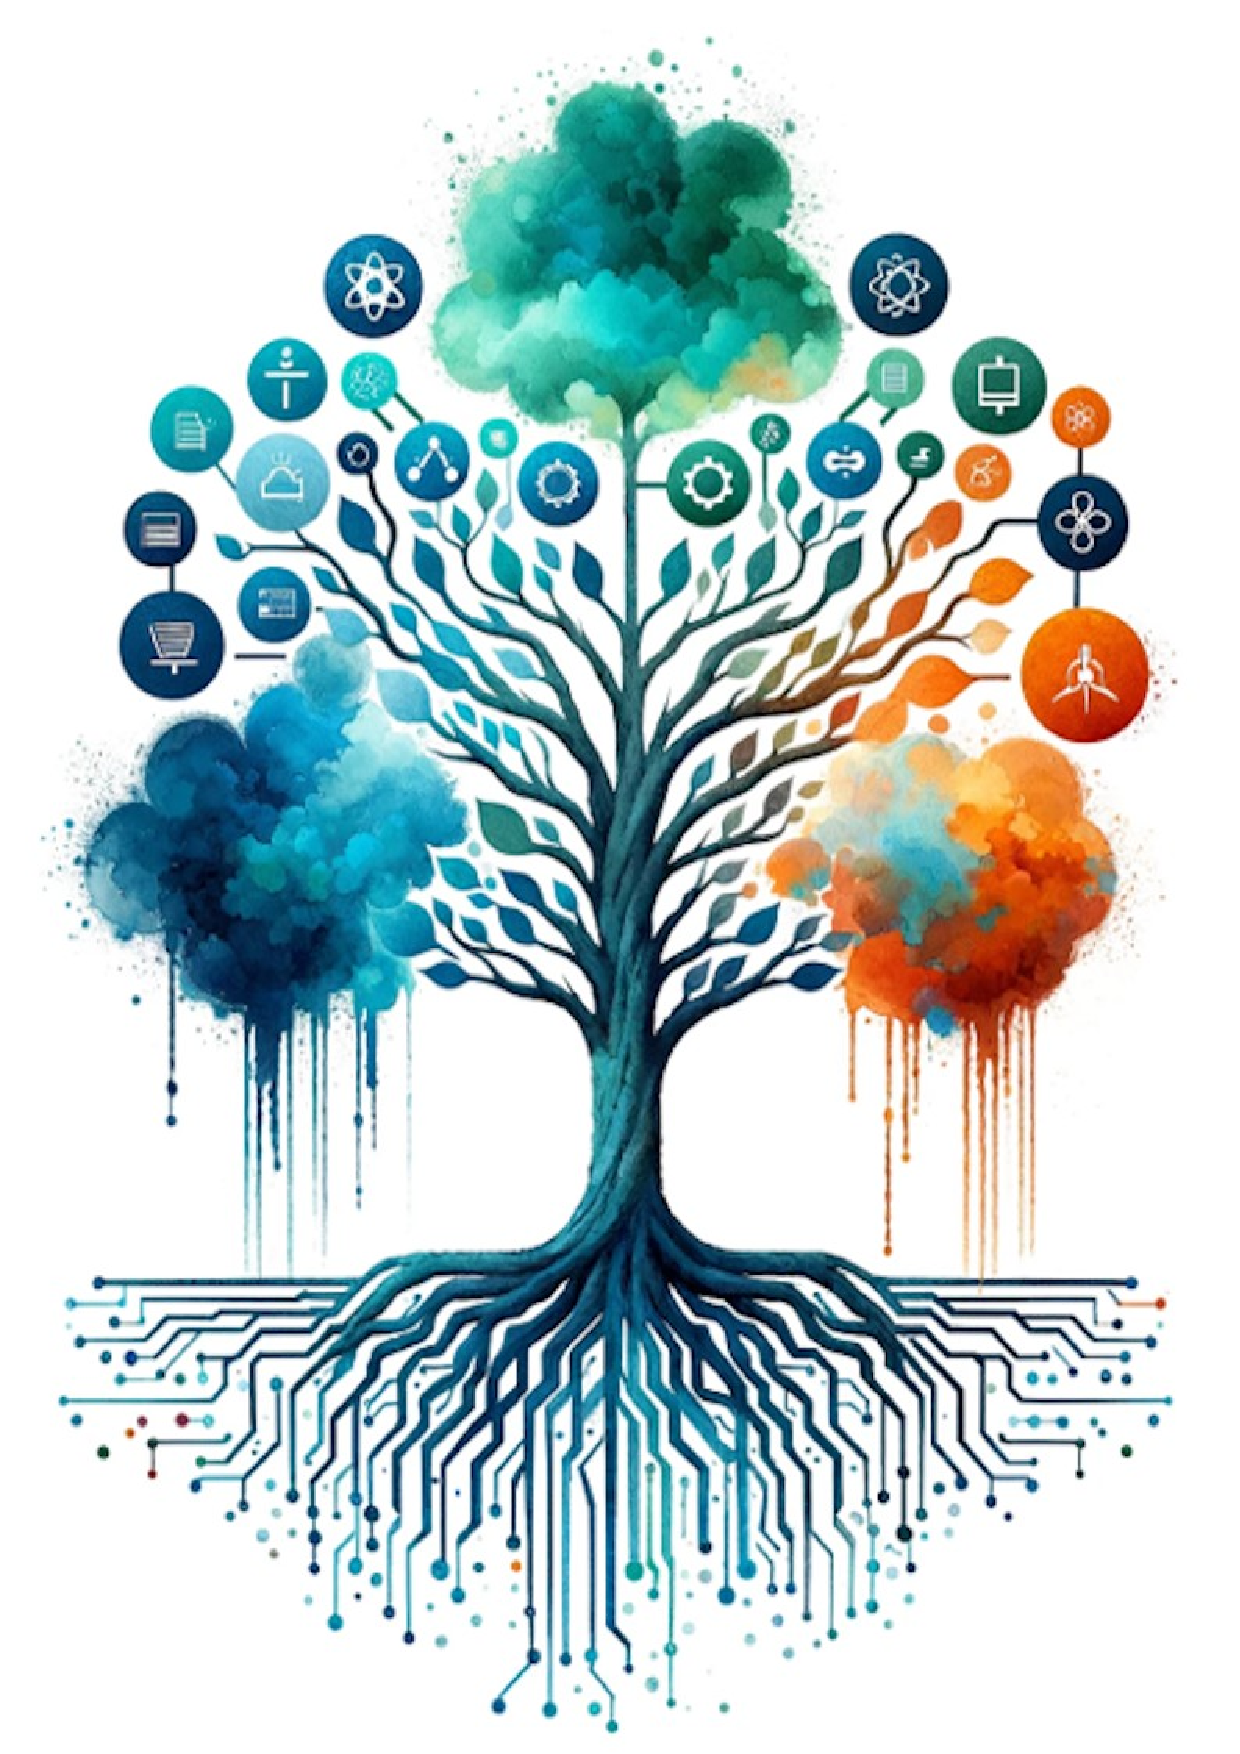
\includepdf[fitpaper=true,pages=-]{img/back-cover}
\pagenumbering{gobble} 

\end{document}
